%%%%%%%%%%%%%%%%%%%%%%%%%%%%%%%%%%%%%%%%%%%%%%%%%%%%%%%%%%%%%%%%%%%%%%%%%%%%%%%%
%
% Template license:
% CC BY-NC-SA 3.0 (http://creativecommons.org/licenses/by-nc-sa/3.0/)
%
%%%%%%%%%%%%%%%%%%%%%%%%%%%%%%%%%%%%%%%%%%%%%%%%%%%%%%%%%%%%%%%%%%%%%%%%%%%%%%%%

%----------------------------------------------------------------------------------------
%	PACKAGES AND OTHER DOCUMENT CONFIGURATIONS
%----------------------------------------------------------------------------------------

\documentclass[
openany,
11pt, % The default document font size, options: 10pt, 11pt, 12pt
%oneside, % Two side (alternating margins) for binding by default, uncomment to switch to one side
%chapterinoneline,% Have the chapter title next to the number in one single line
spanish,
singlespacing, % Single line spacing, alternatives: onehalfspacing or doublespacing
%draft, % Uncomment to enable draft mode (no pictures, no links, overfull hboxes indicated)
%nolistspacing, % If the document is onehalfspacing or doublespacing, uncomment this to set spacing in lists to single
%liststotoc, % Uncomment to add the list of figures/tables/etc to the table of contents
%toctotoc, % Uncomment to add the main table of contents to the table of contents
parskip, % Uncomment to add space between paragraphs
%codirector, % Uncomment to add a codirector to the title page
headsepline, % Uncomment to get a line under the header
]{MastersDoctoralThesis} % The class file specifying the document structure

\usepackage{float}

%----------------------------------------------------------------------------------------
%	INFORMACIÓN DE LA MEMORIA
%----------------------------------------------------------------------------------------

\thesistitle{Sistema de gestión de cultivos aeropónicos} % El títulos de la memoria, se usa en la carátula y se puede usar el cualquier lugar del documento con el comando \ttitle

% Nombre del posgrado, se usa en la carátula y se puede usar el cualquier lugar del documento con el comando \degreename
%\posgrado{Carrera de Especialización en Sistemas Embebidos} 
\posgrado{Carrera de Especialización en Internet de las Cosas} 
%\posgrado{Carrera de Especialización en Intelegencia Artificial}
%\posgrado{Maestría en Sistemas Embebidos} 
%\posgrado{Maestría en Internet de las cosas}

\author{Ing. Nahuel Severini} % Tu nombre, se usa en la carátula y se puede usar el cualquier lugar del documento con el comando \authorname

\director{Mg. Ing. Patricio Bos (FIUBA)} % El nombre del director, se usa en la carátula y se puede usar el cualquier lugar del documento con el comando \dirname
\codirector{Nombre del codirector (pertenencia)} % El nombre del codirector si lo hubiera, se usa en la carátula y se puede usar el cualquier lugar del documento con el comando \codirname.  Para activar este campo se debe descomentar la opción "codirector" en el comando \documentclass, línea 23.

\juradoUNO{Nombre del jurado 1 (pertenencia)} % Nombre y pertenencia del un jurado se usa en la carátula y se puede usar el cualquier lugar del documento con el comando \jur1name
\juradoDOS{Nombre del jurado 2 (pertenencia)} % Nombre y pertenencia del un jurado se usa en la carátula y se puede usar el cualquier lugar del documento con el comando \jur2name
\juradoTRES{Nombre del jurado 3 (pertenencia)} % Nombre y pertenencia del un jurado se usa en la carátula y se puede usar el cualquier lugar del documento con el comando \jur3name

\ciudad{ciudad de Castelar}
%\ciudad{Ciudad Autónoma de Buenos Aires}
%\ciudad{ciudad de Mendoza}

\fechaINICIO{octubre de 2022}
\fechaFINAL{agosto de 2023}


\keywords{Sistemas embebidos, FIUBA} % Keywords for your thesis, print it elsewhere with \keywordnames


\begin{document}


\frontmatter % Use roman page numbering style (i, ii, iii, iv...) for the pre-content pages

\pagestyle{plain} % Default to the plain heading style until the thesis style is called for the body content


%----------------------------------------------------------------------------------------
%	RESUMEN - ABSTRACT 
%----------------------------------------------------------------------------------------

\begin{abstract}
\addchaptertocentry{\abstractname} % Add the abstract to the table of contents
%
%The Thesis Abstract is written here (and usually kept to just this page). The page is kept centered vertically so can expand into the blank space above the title too\ldots
\centering

La presente memoria describe el diseño e implementación de un sistema de control y monitoreo para cultivos aeropónicos, cuyo objetivo es aumentar la productividad y reducir la complejidad en el mantenimiento.

Para lograr este proyecto, se emplearon conocimientos especializados en protocolos de comunicación, arquitectura y pruebas de \emph{software}, arquitectura de datos y ciberseguridad.

%El resumen debe escribirse en uno o dos párrafo.  Debe ser breve y conciso sin ningún elemento de formato en el texto como itálicas o negrita. Tampoco se deben usar siglas ni acrónimos que no resulten obvios para un lector promedio de la memoria, ni referencias bibliográficas o notas al pie de página.  No debe faltar qué es lo que se hizo/logró, qué importancia/valor tiene el proyecto/resultado, qué va a encontrar el lector en la memoria y qué contenidos de la especialización/maestría se aplicaron en el proyecto.

\end{abstract}

%----------------------------------------------------------------------------------------
%	CONTENIDO DE LA MEMORIA  - AGRADECIMIENTOS
%----------------------------------------------------------------------------------------

%\begin{acknowledgements}
%\addchaptertocentry{\acknowledgementname} % Descomentando esta línea se puede agregar los agradecimientos al índice
%\vspace{1.5cm}

%Esta sección es para agradecimientos personales y es totalmente \textbf{OPCIONAL}.  

%\end{acknowledgements}

%----------------------------------------------------------------------------------------
%	LISTA DE CONTENIDOS/FIGURAS/TABLAS
%----------------------------------------------------------------------------------------

\tableofcontents % Prints the main table of contents

\listoffigures % Prints the list of figures

\listoftables % Prints the list of tables


%----------------------------------------------------------------------------------------
%	CONTENIDO DE LA MEMORIA  - DEDICATORIA
%----------------------------------------------------------------------------------------

% \dedicatory{\textbf{Dedicado a... [OPCIONAL]}}  % escribir acá si se desea una dedicatoria

%----------------------------------------------------------------------------------------
%	CONTENIDO DE LA MEMORIA  - CAPÍTULOS
%----------------------------------------------------------------------------------------

\mainmatter % Begin numeric (1,2,3...) page numbering

\pagestyle{thesis} % Return the page headers back to the "thesis" style

% Incluir los capítulos como archivos separados desde la carpeta Chapters

% Chapter 1

\chapter{Introducción general} % Main chapter title

\label{Chapter1} % For referencing the chapter elsewhere, use \ref{Chapter1} 
\label{IntroGeneral}

%----------------------------------------------------------------------------------------

% Define some commands to keep the formatting separated from the content 
\newcommand{\keyword}[1]{\textbf{#1}}
\newcommand{\tabhead}[1]{\textbf{#1}}
\newcommand{\code}[1]{\texttt{#1}}
\newcommand{\file}[1]{\texttt{\bfseries#1}}
\newcommand{\option}[1]{\texttt{\itshape#1}}
\newcommand{\grados}{$^{\circ}$}

%----------------------------------------------------------------------------------------

%\section{Introducción}

En este capítulo se presenta una introducción al concepto de aeroponía y sus principales ventajas. Además, se describe el estado del arte y se exponen los objetivos, alcance y requerimientos del trabajo.


%----------------------------------------------------------------------------------------
\section{Aeroponía}

La aeroponía es una técnica de cultivo de plantas en la que las raíces cuelgan suspendidas en el aire mientras se les entrega una solución nutritiva en forma de una fina niebla \citep{WEBSITE:AEROPONIA1}. Como se usa agua para transmitir nutrientes, a veces se habla de los cultivos aeropónicos como de tipo hidropónico \citep{WEBSITE:HIDROPONIA}.

En la figura \ref{fig:zonaDeCultivoAeroponica} se presenta un típico ejemplo de una zona de cultivo aeropónica, en la que se puede observar el posicionamiento de las plantas y su sistema de nebulización.

\begin{figure}[htbp]
	\centering
	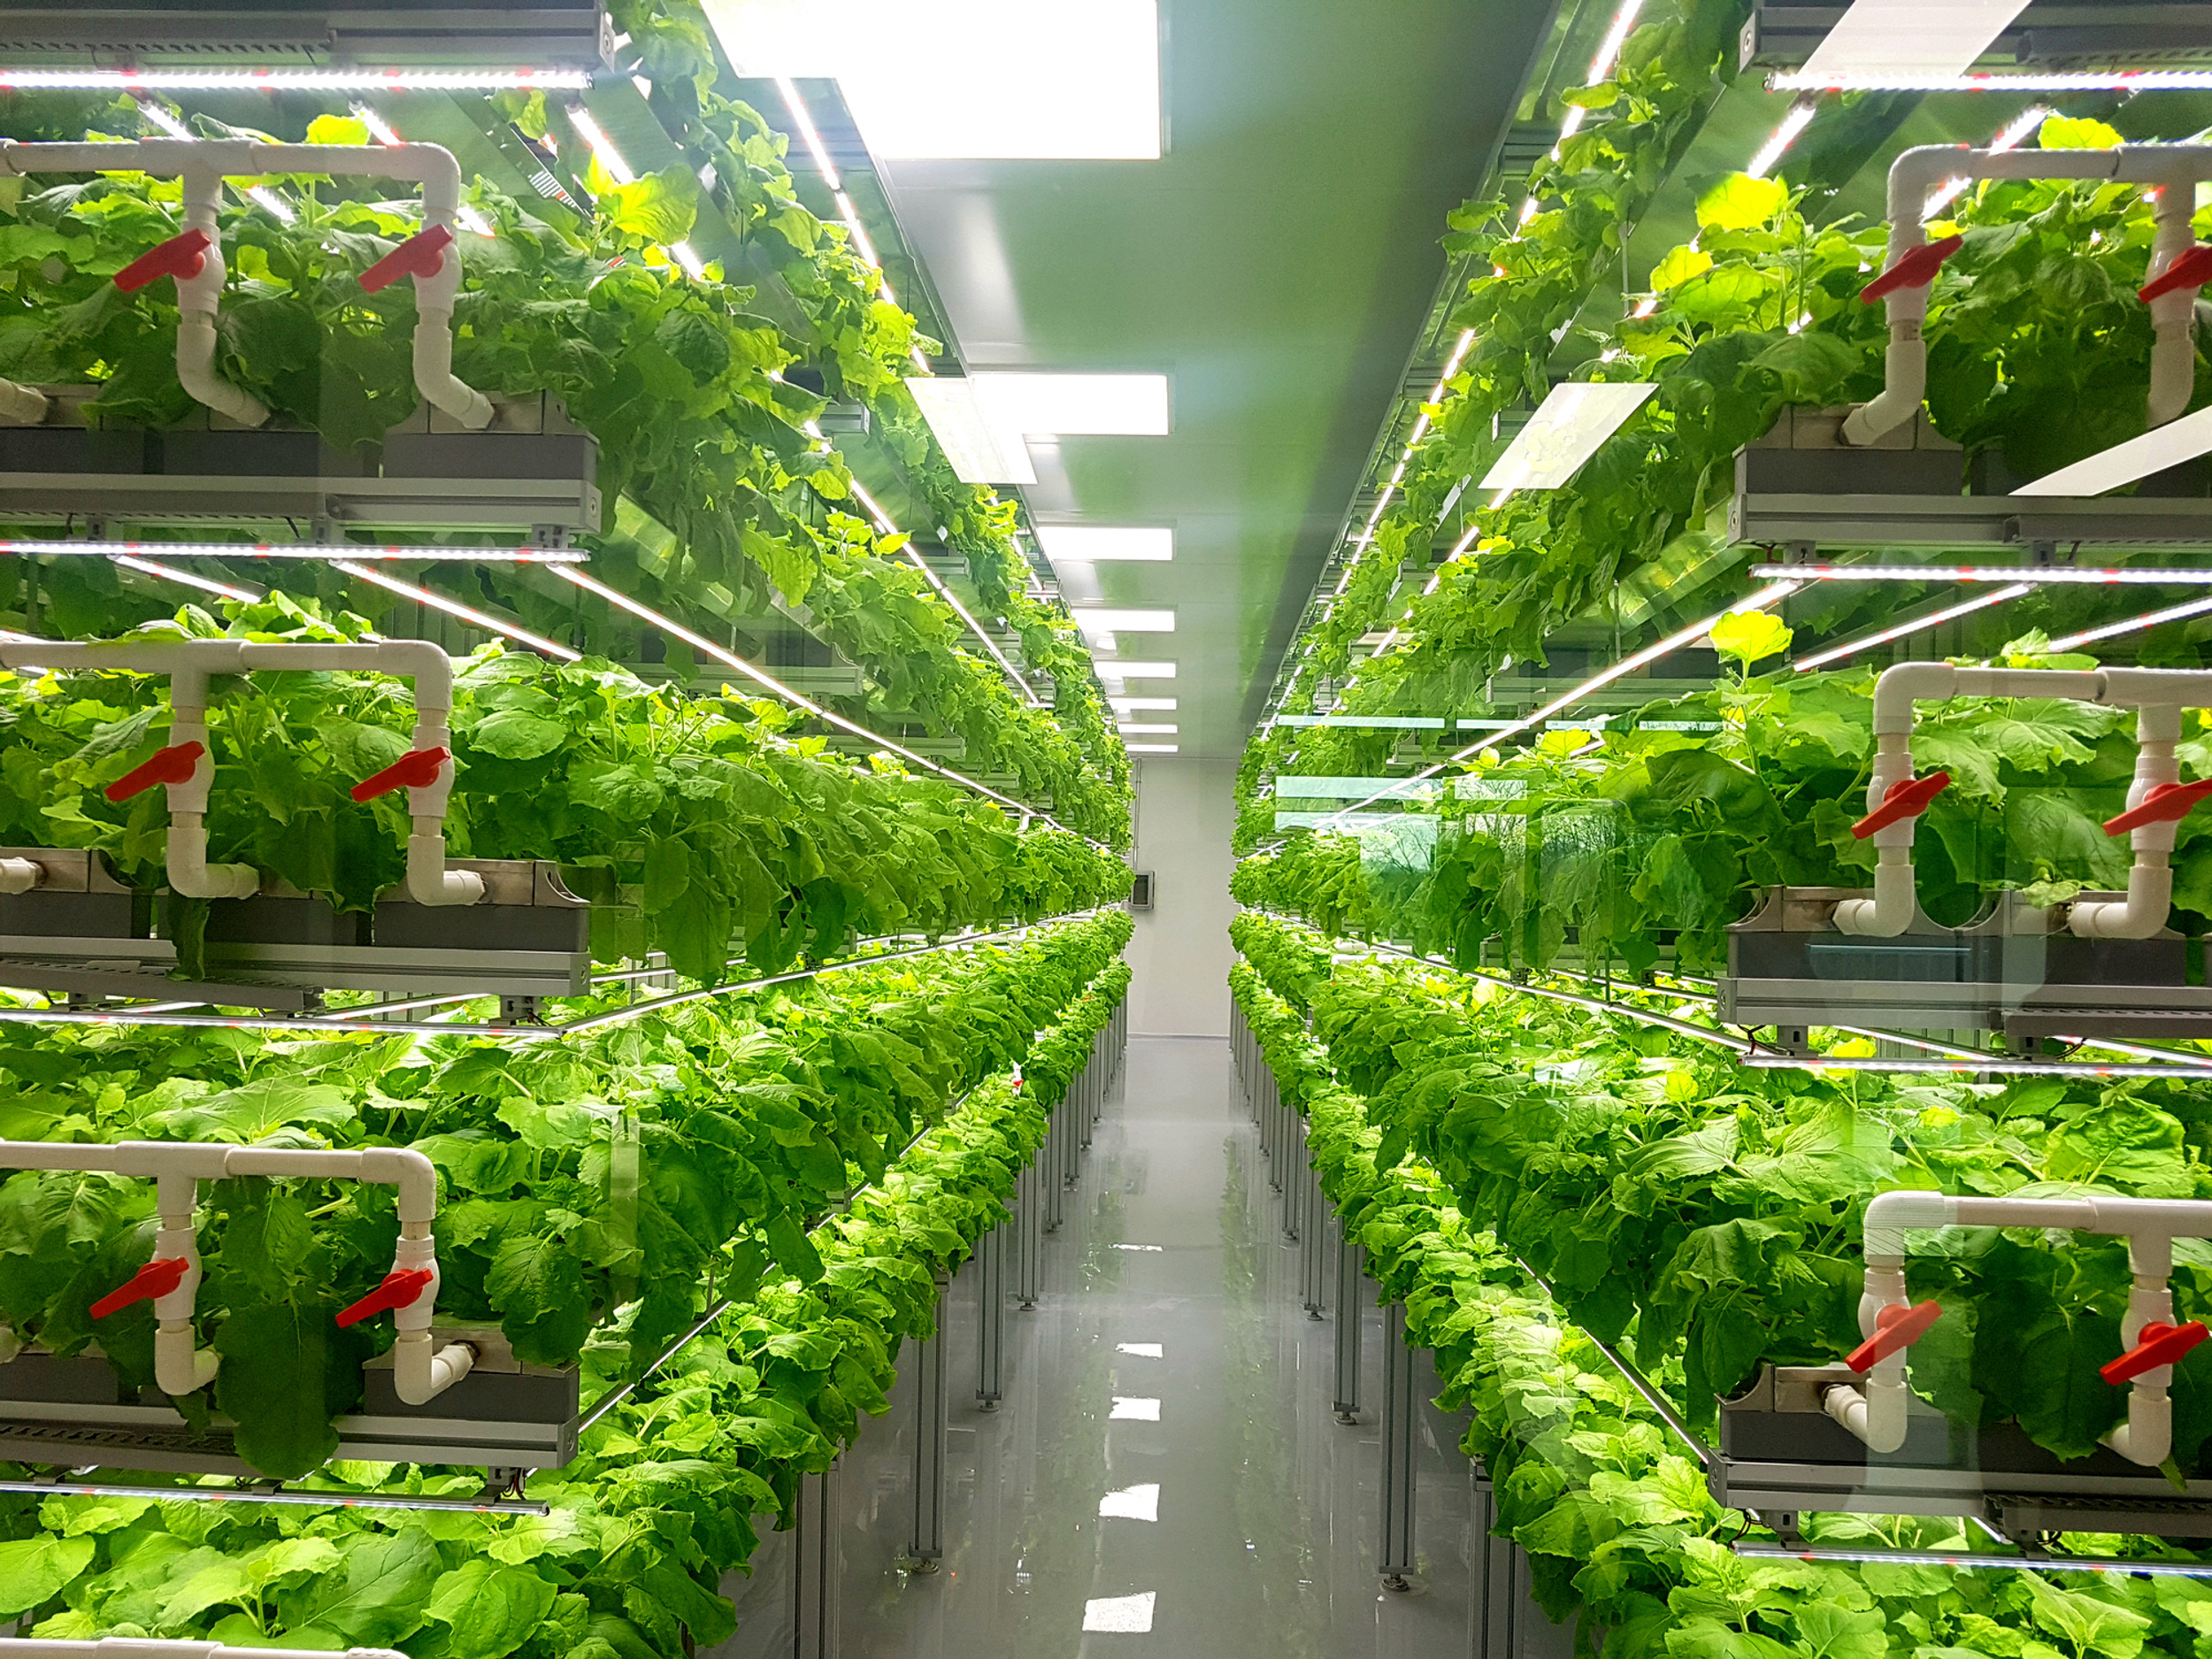
\includegraphics[width=.9\textwidth]{./Figures/Zona de cultivo aeroponica.jpg}
	\caption{Zona de cultivo aeropónica\protect\footnotemark.}
	\label{fig:zonaDeCultivoAeroponica}
\end{figure}


\footnotetext{Imagen tomada de \url{https://www.acquagarden.com.ar/aeroponia}}

El crecimiento aeropónico es considerado seguro y ecológico por producir cosechas de forma natural manteniendo las plantas saludables. Su principal ventaja ecológica frente a otros sistemas es la conservación de agua, energía y nutrientes  \citep{WEBSITE:AEROPONIA2}. 

Una de sus características más importante es que requieren poco contacto físico con el sistema radicular del cultivo, para no interferir con el crecimiento y expansión natural de las raíces y lograr un intercambio limpio de agua y aire. Por esta razón, en comparación con las plantas hidropónicas, los cultivos tienden a crecer más rápido y a absorber más nutrientes, ya que están expuestas a más oxígeno. A su vez, hay menos amenazas de enfermedades alrededor de la zona de la raíz ya que no hay lugar para que residan los desechos \citep{WEBSITE:AEROPONIA3}.

En la figura \ref{fig:diagramaAeroponia} puede observarse el diagrama de un cultivo aeropónico junto con su proceso de nebulización. 

\begin{figure}[htbp]
	\centering
	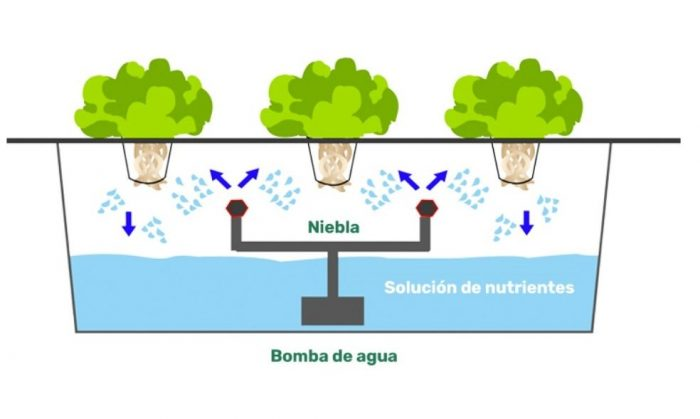
\includegraphics[width=.9\textwidth]{./Figures/Diagrama Aeroponia.jpg}
	\caption{Diagrama aeroponía\protect\footnotemark.}
	\label{fig:diagramaAeroponia}
\end{figure}

\footnotetext{Imagen tomada de \url{https://hidroponia24.com/sistemas-hidroponicos/aeroponia/}}

Sin embargo, para lograr que un sistema aeropónico tenga éxito es necesario que se controlen múltiples parámetros que son vitales para el correcto desarrollo de los cultivos, como por ejemplo la temperatura y caudal de la solución nutritiva a utilizar en el proceso de nebulización, la temperatura y humedad del ambiente, el nivel de dióxido de carbono y el nivel de iluminación entre otros \citep{WEBSITE:AEROPONIA4}.

%----------------------------------------------------------------------------------------

\section{Objetivos y alcance}

El propósito de este trabajo es el diseño, desarrollo e implementación de un sistema que permita la gestión de cultivos aeropónicos, con el objetivo de incrementar su productividad y reducir la dificultad de mantenimiento.

El trabajo incluye:
\begin{itemize}
	\item Diseño y desarrollo de una aplicación SSR (del inglés \textit{server-side rendering}) \citep{WEBSITE:SSR} que permita la interacción del usuario con el sistema.
	\item Diseño y desarrollo de una API (del inglés \textit{application programming interface}) \citep{WEBSITE:API} REST (del inglés \textit{representational state transfer}) \citep{WEBSITE:REST} que permita la comunicación por medio de los protocolos HTTP (del inglés \textit{Hypertext Transfer Protocol}) \citep{WEBSITE:HTTP}, MQTT (del inglés \textit{Message Queue Telemetry Transport}) \citep{WEBSITE:MQTT} y WebSocket \citep{WEBSITE:WEBSOCKET}.
	\item Diseño de un modelo de datos a utilizar por el DaaS (del inglés \textit{data as a service}) \citep{WEBSITE:DAAS} que permita almacenar los datos.
	\item Configuración y despliegue del DaaS.
	\item Diseño y desarrollo de un \textit{broker} que permita la comunicación por medio de los protocolos MQTT y WebSockets.
	\item Desarrollo del \emph{software} del microcontrolador para realizar una prueba de concepto.
\end{itemize}

El trabajo no incluye:
\begin{itemize}
	\item Diseño de un gabinete para el microcontrolador y los sensores a utilizar.
	\item Desarrollo del \emph{software} final del microcontrolador.
	\item Uso de certificados TLS (del inglés \textit{Transport Layer Security}) \citep{WEBSITE:TLS} emitidos por autoridades de confianza.
	\item Despliegue del servidor en un entorno \textit{cloud}.
	\item Accionar la bomba y el nebulizador del cultivo aeropónico por medio del sistema.
\end{itemize}

%----------------------------------------------------------------------------------------

\section{Estado del arte}

Se llevó a cabo una búsqueda de sistemas similares en el mercado nacional, pero solo se encontró un producto que ofrece características comparables o que cuente con documentación suficiente para una comparación adecuada. Por este motivo, se decidió incluir en la búsqueda sistemas del mercado internacional y publicaciones científicas. 

En la tabla \ref{tab:comparativaSolucionesNacionalesInternacionales} se presenta la comparación de las características y funcionalidades de los sistemas comerciales encontrados en el mercado nacional e internacional.

My Autogrow \citep{WEBSITE:MYAUTOGROW} permite la automatización y control de todo tipo de sistemas agrícolas. Los datos del sistema son obtenidos por medio de sensores y se almacenan en una plataforma \emph{cloud}. El sistema utiliza MQTT y HTTP como protocolos de comunicación. Los usuarios acceden al sistema mediante una aplicación web, cuyas principales características se detallan a continuación: 

\begin{itemize}
	\item Histórico de mediciones con filtros.
	\item Administración de alertas.
	\item Administración de áreas de cultivo.
	\item Administración de sistema de fertirrigación \citep{WEBSITE:FERTIRRIGACION}.
	\item Administración de sistema de riego.
	\item Visualización de gráficos.
\end{itemize}

Smartcultiva \citep{WEBSITE:PLIOT} permite la obtención de datos y métricas mediante una red de sensores instalados en la zona de cultivo. Los datos son enviados mediante MQTT y se almacenan en una plataforma \emph{cloud}. Los usuarios acceden al sistema mediante una aplicación web o móvil, cuyas principales características se detallan a continuación: 

\begin{itemize}
	\item Histórico de mediciones con filtros.
	\item Administración de dispositivos externos.
	\item Exportación de datos a diferentes formatos.
	\item Administración de alertas.
	\item Automatización de acciones frente al disparo de alertas.
	\item Visualización de gráficos.
\end{itemize}

Es importante notar que My Autogrow y Smartcultiva trabajan con sensores propietarios solamente.

\begin{table}[H]
	\centering
	\caption[Comparativa entre soluciones comerciales similares]{Comparativa entre soluciones comerciales similares.}
	\begin{tabular}{l c c c}    
		\toprule
		\textbf{Funcionalidad} & \textbf{Smartcultiva} & \textbf{My Autogrow} \\
		\midrule
		MQTT & Sí & Sí \\
		Sistema de alertas & Sí & Sí \\
		Acciones automatizadas & Sí & No \\
		Notificaciones \emph{push} \citep{WEBSITE:NOTIFICACIONESPUSH} & No & No \\
		Notificaciones \textit{email} & Sí & Sí \\
		Accionamiento de dispositivos externos & Sí & No \\
		Escalabilidad en sensores & Limitado & Limitado \\
		Tipo de aplicación & Móvil y web & Web \\
		\bottomrule
		\hline
	\end{tabular}
	\label{tab:comparativaSolucionesNacionalesInternacionales}
\end{table}

En la tabla \ref{tab:comparativaSolucionesPublicacionesCientificas} se presenta la comparación de las características y funcionalidades de los sistemas encontrados en publicaciones científicas.

\emph{Monitoring Soil and Ambient Parameters in the IoT Precision Agriculture Scenario: An Original Modeling Approach Dedicated to Low-Cost Soil Water Content Sensors} \citep{WEBSITE:SOLUCIONSIMILARCIENTIFICA2} presenta el desarrollo de un sistema de monitoreo de parámetros ambientales y del suelo enfocado en la agricultura. Los datos del sistema son obtenidos por nodos a nivel planta y a nivel de invernadero y enviados a un \emph{gateway} mediante el protocolo LoRa (del inglés \textit{long range}) \citep{WEBSITE:LORA}. El \emph{gateway} es el encargado de utilizar MQTT para enviar los datos a una plataforma \emph{cloud}. Los usuarios acceden al sistema mediante una plataforma web que permite monitorear los datos obtenidos y visualizar gráficos.

\emph{A Smart Agricultural System Based on PLC and a CloudComputing Web Application Using LoRa and LoRaWan} \citep{WEBSITE:SOLUCIONSIMILARCIENTIFICA3} presenta el desarrollo de un sistema compuesto por dos tipos de nodos: a nivel granja y a nivel depósito. Los nodos envían los datos obtenidos a un \emph{gateway} mediante el protocolo LoRa. El \emph{gateway} es el encargado de enviar los datos a una plataforma \emph{cloud}. Los usuarios acceden al sistema mediante una plataforma web que permite monitorear y exportar los datos obtenidos, administrar el sistema de alertas y visualizar gráficos. El sistema envía las notificaciones de las alertas mediante \textit{email} y un \textit{bot} \citep{WEBSITE:BOT} de Telegram \citep{WEBSITE:TELEGRAM}.

Se considera que la escalabilidad para incorporar nuevos sensores en las dos soluciones anteriores es media, debido a las estructuras planteadas a nivel aplicación. 

Es importante destacar que ambas soluciones fueron ejecutadas y probadas, es decir no son publicaciones teóricas. 

\begin{table}[H]
	\centering
	\caption[Comparativa entre soluciones similares encontradas en publicaciones científicas]{Comparativa entre soluciones similares encontradas en publicaciones científicas.}
	\begin{tabular}{l c c}    
		\toprule
		\textbf{Funcionalidad} & \textbf{\textit{Monitoring Soil (...)}} & \textbf{\textit{A Smart (...)}}  \\
		\midrule
		MQTT & Sí & No  \\
		LoRa & Sí & Sí  \\
		Sistema de alertas & No & Sí \\
		Acciones automatizadas & No & No \\
		Notificaciones \emph{push} & No & No \\
		Notificaciones \textit{email} & No & Sí \\
		Accionamiento de dispositivos externos & No & No \\
		Escalabilidad en sensores & Media & Media \\
		Tipo de aplicación & Web & Web \\
		\bottomrule
		\hline
	\end{tabular}
	\label{tab:comparativaSolucionesPublicacionesCientificas}
\end{table}

%----------------------------------------------------------------------------------------

\section{Requerimientos}

Se organizaron los requerimientos en secciones de acuerdo con su relación a las distintas áreas del trabajo.

\begin{enumerate}

	\item Requerimientos asociados a la aplicación SSR:
		\begin{enumerate}
			\item Deberá estar configurada para utilizar certificados TLS.
			\item Deberá estar configurada para poder enviar y recibir información mediante los protocolos HTTP y WebSockets.
			\item Deberá incluir el renderizado de la aplicación web en el servidor.
			\item Deberá contar con una interfaz de usuario para permitir el inicio de sesión en el sistema.
			\item Deberá contar con una interfaz de usuario para permitir la creación y modificación de usuarios.
			\item Deberá contar con las interfaces de usuario para realizar el CRUD (del inglés \textit{create, read, update and delete}) \citep{WEBSITE:CRUD} de zonas.
			\item Deberá contar con las interfaces de usuario para realizar el CRUD de alarmas.
			\item Deberá validar los datos recibidos en cada uno de los formularios de las interfaces de usuario.
			\item Deberá contar con una interfaz de usuario para monitorear en tiempo real el histórico de las mediciones obtenidas.
			\item Deberá contar con una interfaz de usuario para permitir la activación de los \textit{relays} disponibles.
			\item Deberá contar con un módulo para controlar el acceso a las interfaces de usuario según su nivel de autenticación.
		\end{enumerate}
		
	\item Requerimientos asociados a la API REST:
		\begin{enumerate}
			\item Deberá estar configurada para utilizar certificados TLS.
			\item Deberá estar configurada para poder enviar y recibir información mediante los protocolos HTTP, WebSockets y MQTT.
			\item Deberá incluir los \textit{endpoints} para realizar la alta y la modificación de usuarios.
			\item Deberá incluir los \textit{endpoints} para realizar el CRUD de zonas.
			\item Deberá incluir los \textit{endpoints} para realizar el CRUD de alarmas.
			\item Deberá incluir un \textit{endpoint} para obtener el histórico de mediciones.
			\item Deberá incluir un \textit{endpoint} para la activación de los \textit{relays} \citep{WEBSITE:RELAY} disponibles.
			\item Deberá incluir un módulo de autenticación y autorización de usuarios con sus respectivos \textit{endpoints}.
			\item Deberá validar los datos recibidos en cada uno de los \textit{endpoints}.
		\end{enumerate}
		
	\item Requerimientos asociados al DaaS:
		\begin{enumerate}
			\item Deberá ser configurado y desplegado en un entorno \textit{cloud}.
			\item Deberá persistir la información de los usuarios: id, \textit{email}, contraseña y fecha y hora de creación.
			\item Deberá persistir la información de las zonas de cultivo: id, nombre, localización, dispositivo, usuario, alarmas asociadas y última medición.
			\item Deberá persistir la información de las mediciones: id, temperatura del ambiente, humedad del ambiente, temperatura de la solución nutritiva, nivel de dióxido de carbono, nivel de iluminación, fecha con la hora de creación del registro, usuario, zona y dispositivo.
			\item Deberá persistir la información de los dispositivos: id, nombre, contraseña, estado del módulo de \textit{relay}.
			\item Deberá persistir la información de las alarmas: id, nombre, condición, zona y usuario.
		\end{enumerate}
		
	\item Requerimientos asociados al \textit{broker}:
		\begin{enumerate}
			\item Deberá estar configurado para utilizar certificados TLS.
			\item Deberá estar configurado para poder enviar y recibir información mediante los protocolos MQTT y WebSockets.
		    \item Deberá contar con un módulo de autenticación y autorización de dispositivos.
			\item Deberá permitir la conexión de múltiples microcontroladores de manera simultánea.
			\item Deberá permitir la activación de los \textit{relays} disponibles.
			\item Deberá analizar la información recibida, validarla y en caso de ser necesario almacenarla en el DaaS.
			\item Deberá enviar una notificación al usuario en caso de que la condición de una alarma predefinida se cumpla.
		\end{enumerate}
		
	\item Requerimientos asociados al microcontrolador y sensores:
		\begin{enumerate}
			\item Deberá estar configurado para utilizar certificados TLS.
			\item Deberá utilizar el protocolo MQTT para enviar y recibir información.
		    \item Deberá tener configurado las credenciales necesarias para unirse a la red local mediante Wi-Fi  \citep{WEBSITE:WIFI}.
			\item Deberá permitir accionar el módulo de \textit{relay}.
			\item Deberá obtener la temperatura del ambiente con una exactitud de ±0,5 °C (Celsius) y una resolución de 0,1 °C en un rango de operación entre los 15 °C y 35 °C. La frecuencia de muestreo deberá ser de una muestra cada 5 minutos.
			\item Deberá obtener la humedad del ambiente con una exactitud de ±2{\%} RH (humedad relativa) y una resolución de 0,1{\%} RH en un rango de operación de 40-100{\%} RH. La frecuencia de muestreo deberá ser de una muestra cada 5 minutos.
			\item Deberá obtener la temperatura de la solución nutritiva con una exactitud de ±0,5 °C en un rango de operación entre los 15 °C y 35 °C. La frecuencia de muestreo deberá ser de una muestra cada 5 minutos.
			\item Deberá obtener el nivel de dióxido de carbono del ambiente con una exactitud de ±15{\%} en un rango de operación de 400-1000 PPM (partes por millón). La frecuencia de muestreo deberá ser de una muestra cada 5 minutos.
			\item Deberá obtener el nivel de iluminación en el ambiente con un rango de operación de 3000-50000 lx. La frecuencia de muestreo deberá ser de una muestra cada 5 minutos.
			\item Deberá obtener el caudal líquido con una exactitud de ±10{\%} en un rango de operación de 1-30 litros por minuto.
		\end{enumerate}	
		
	\item Requerimientos asociados a las pruebas:
		\begin{enumerate}
			\item La aplicación SSR deberá contar con al menos 70{\%} de cobertura de código \citep{WEBSITE:TESTCOVERAGE}.
			\item La API REST deberá contar con al menos 70{\%} de cobertura de código.
		\end{enumerate}					
\end{enumerate}

En la figura \ref{fig:diagramaGeneralDeLaSolucion} se presenta un diagrama general de la solución y los componentes que la forman.

Para cada zona de cultivo aeropónica se emplea un microcontrolador, responsable de recopilar los datos de los sensores y transmitirlos al servidor, el cual se encarga de analizar y validar la información recibida y en caso necesario enviarla al DaaS para ser almacenada.

\begin{figure}[H]
	\centering
	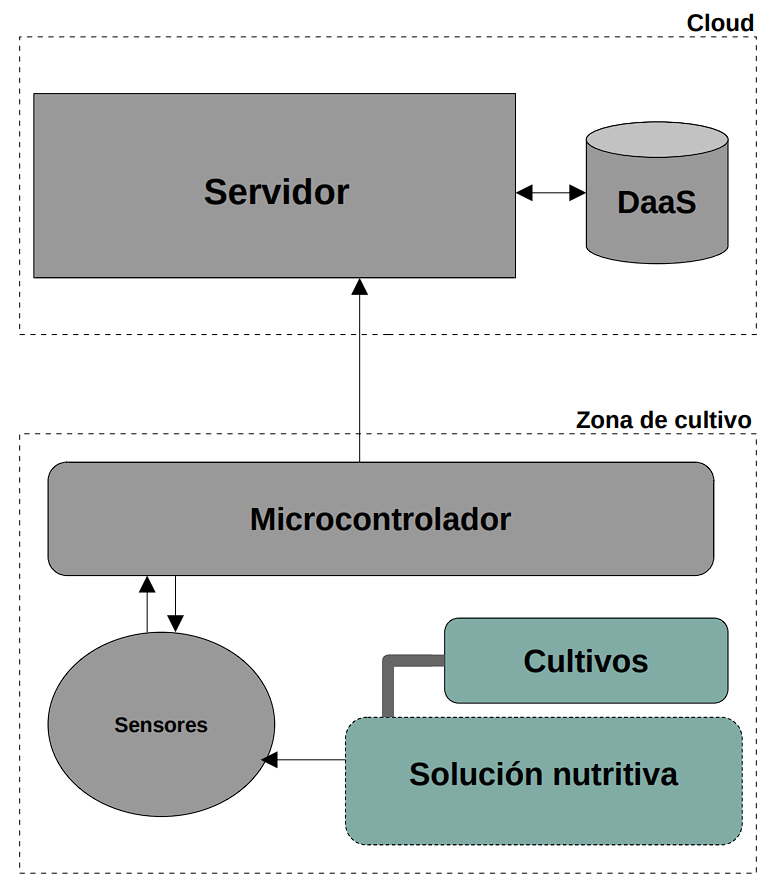
\includegraphics[width=.8\textwidth]{./Figures/Diagrama general de la solucion v2.png}
	\caption{Diagrama general de la solución.}
	\label{fig:diagramaGeneralDeLaSolucion}
\end{figure}
\chapter{Introducción específica} % Main chapter title

\label{Chapter2}

%----------------------------------------------------------------------------------------
%	SECTION 1
%----------------------------------------------------------------------------------------

En este capítulo se introducen los protocolos de comunicación, los diversos componentes de hardware y las herramientas de software utilizadas para el desarrollo del trabajo. 

\section{Protocolos de comunicación}

\subsection{\emph{Hypertext Transfer Protocol}}

HTTP es un protocolo de la capa de aplicación \citep{WEBSITE:CAPADEAPLICACION} para la transmisión de documentos hipermedia, como HTML (del inglés \textit{HyperText Markup Language}) \citep{WEBSITE:HTML}. Fue diseñado para la comunicación entre los navegadores y servidores web, aunque se puede utilizar para otros propósitos también. 

Sigue el clásico modelo cliente-servidor \citep{WEBSITE:CLIENTESERVIDOR}, en el que un cliente establece una conexión con el servidor, realiza una petición y espera hasta que recibe una respuesta del mismo. 

Se trata de un protocolo sin estados \citep{WEBSITE:PROTOCOLOSINESTADO}, lo cual significa que el servidor no guarda información entre dos peticiones distintas. 

Aunque en la mayoría de casos se basa en una conexión del tipo TCP/IP (del inglés \textit{Transmission Control Protocol/Internet Protocol}) \citep{WEBSITE:TCPIP} y se puede usar sobre cualquier capa de transporte \citep{WEBSITE:CAPADETRANSPORTE} segura o de confianza.

Las características claves de HTTP son:
\begin{itemize}
\item Es sencillo: HTTP está pensado y desarrollado para ser leído y fácilmente interpretado por sus usuarios. Esto facilita depurar errores y reduce su curva de aprendizaje.
\item Es extensible: las cabeceras de HTTP han hecho que este protocolo sea fácil de ampliar y de experimentar con él.
\item Es un protocolo con sesiones pero sin estados.
\end{itemize}

En la figura \ref{fig:ejemploDeComunicacionEnHTTP} se presenta un ejemplo de comunicación HTTP en el que puede observarse como interactúa un cliente con el servidor.

\begin{figure}[H]
	\centering
	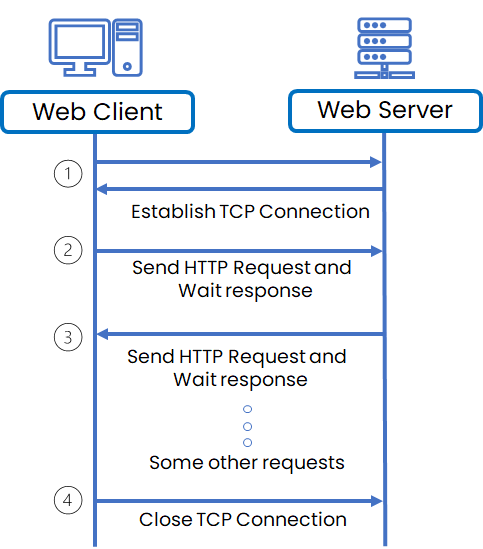
\includegraphics[width=.6\textwidth]{./Figures/Ejemplo de comunicacion en HTTP.png}
	\caption{Ejemplo de comunicacion en HTTP\protect\footnotemark.}
	\label{fig:ejemploDeComunicacionEnHTTP}
\end{figure}

\footnotetext{Imagen tomada de \newline  \url{https://www.ionos.co.uk/digitalguide/hosting/technical-matters/what-is-http/}}

La versión encriptada de HTTP se llama HTTPS (del inglés \textit{Hypertext Transfer Protocol Secure}) \citep{WEBSITE:HTTPS}. Normalmente utiliza TLS para cifrar toda la comunicación entre un cliente y un servidor. Esta conexión segura permite a los clientes intercambiar datos confidenciales de forma segura con un servidor, por ejemplo, para actividades bancarias o compras en línea.

\subsection{\emph{Message Queue Telemetry Transport}}

MQTT es un protocolo de mensajería basado en estándares o conjuntos de reglas, que se utiliza para la comunicación de un equipo a otro. 

Los sensores inteligentes, los dispositivos portátiles y otros dispositivos IoT (del inglés \textit{Internet of Things}) \citep{WEBSITE:IOT} generalmente tienen que transmitir y recibir datos a través de una red con recursos restringidos y un ancho de banda limitado. Estos dispositivos IoT utilizan MQTT para la transmisión de datos, ya que resulta fácil de implementar y puede comunicar datos IoT de manera eficiente. MQTT admite mensajería bidireccional entre dispositivos y una plataforma \textit{cloud}.

El protocolo MQTT funciona según los principios del modelo de publicación o suscripción. Sus componentes son los siguientes:
\begin{itemize}
\item Cliente: es cualquier dispositivo que ejecuta una biblioteca MQTT. Si el cliente envía mensajes, actúa como editor y si recibe mensajes, actúa como receptor.
\item Agente o \emph{broker}: es el sistema que coordina los mensajes entre los diferentes clientes. Además, se encarga de otras tareas como la autorización y autenticación de los clientes, identificar a los clientes suscritos a cada tema y el envío de sus mensajes y controlar los mensajes perdidos y las sesiones del cliente. 
\item Conexión: los clientes inician la conexión al enviar un mensaje CONECTAR al agente MQTT. El agente confirma que se ha establecido una conexión al responder con un mensaje CONNACK. Los clientes nunca se conectan entre sí, solo con el agente.
\end{itemize}

En la figura \ref{fig:ejemploDeComunicacionEnMQTT} se presenta un ejemplo de comunicación MQTT en el que puede observarse como interactúan cada uno de los componentes del protocolo.
 
\begin{figure}[H]
	\centering
	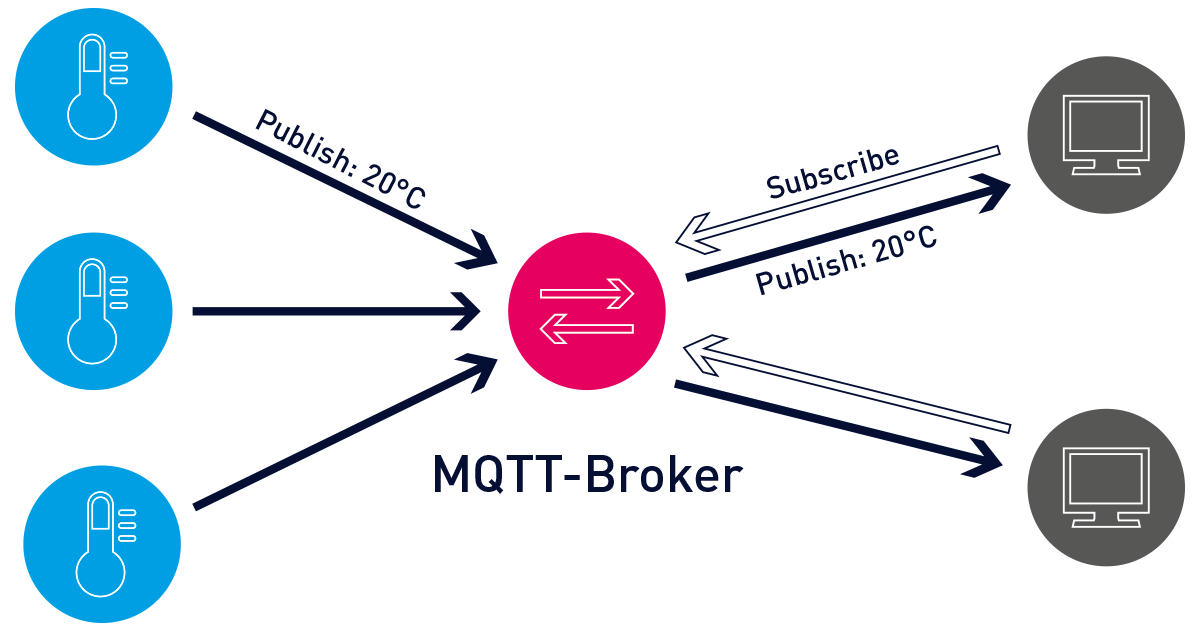
\includegraphics[width=.8\textwidth]{./Figures/Ejemplo de comunicacion en MQTT.jpg}
	\caption{Ejemplo de comunicación en MQTT\protect\footnotemark.}
	\label{fig:ejemploDeComunicacionEnMQTT}
\end{figure}

\footnotetext{Imagen tomada de \url{https://www.paessler.com/es/it-explained/mqtt}}

La comunicación MQTT utiliza el protocolo SSL para proteger los datos confidenciales que transmiten los dispositivos IoT. Puede implementar la identidad, la autenticación y la autorización entre los clientes y el agente mediante certificados SSL y contraseñas. El agente MQTT normalmente autentica a los clientes mediante sus contraseñas e identificadores únicos. En la mayoría de las implementaciones, el cliente autentica el servidor con certificados o búsquedas de DNS \citep{WEBSITE:DNS}. También puede implementar protocolos de cifrado con MQTT. 

\subsection{WebSocket}

WebSocket es una tecnología que proporciona un canal de comunicación bidireccional y full-dúplex \citep{WEBSITE:FULLDUPLEX} sobre un único \textit{socket} TCP \citep{WEBSITE:TCP}. Está diseñada para ser implementada en navegadores y servidores web, pero puede utilizarse por cualquier aplicación cliente/servidor. Además, puede utilizar SSL para las conexiones seguras y la transmisión de datos.

WebSocket utiliza un secuencia de solicitud-respuesta HTTP estándar para establecer una conexión. Una vez formada, la API WebSocket proporciona una interfaz de lectura y escritura de datos entre las partes de modo dúplex asíncrono. También proporciona una interfaz para el cierre asíncrono de la conexión desde cualquier lado.

En la figura \ref{fig:ejemploDeComunicacionEnWebSocket} se presenta un ejemplo de comunicación WebSocket, en el que puede observarse cómo interactúan el cliente y el servidor.

\begin{figure}[H]
	\centering
	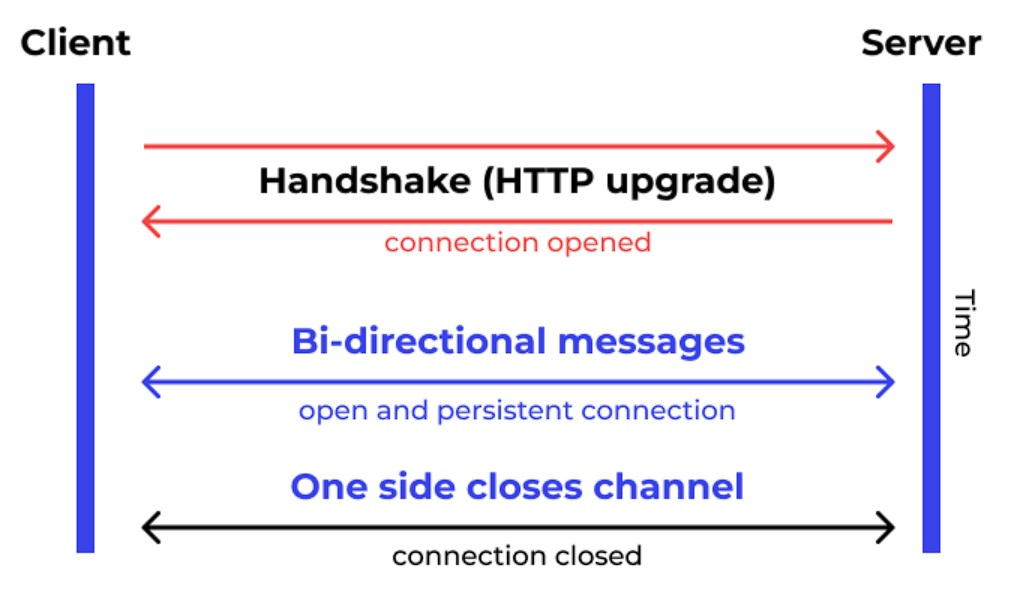
\includegraphics[width=.9\textwidth]{./Figures/Ejemplo de comunicacion en WebSocket.jpg}
	\caption{Ejemplo de comunicación en WebSocket\protect\footnotemark.}
	\label{fig:ejemploDeComunicacionEnWebSocket}
\end{figure}

\footnotetext{Imagen tomada de \newline \url{https://www.wallarm.com/what/a-simple-explanation-of-what-a-websocket-is}}

\section{Componentes de \emph{hardware}}

\subsection{Microcontrolador}

ESP32 \citep{WEBSITE:ESP32} es la denominación de una familia de chips SoC (del inglés \textit{system on a chip}) \citep{WEBSITE:SOC} de bajo coste y consumo de energía. Los integrados cuentan con tecnología Wi-Fi y Bluetooth \citep{WEBSITE:BLUETOOTH} de modo dual integrada. El ESP32 emplea un microprocesador Tensilica Xtensa LX6 en sus variantes de simple y doble núcleo e incluye interruptores de antena, balun de radiofrecuencia, amplificador de potencia, amplificador receptor de bajo ruido, filtros y módulos de administración de energía.

La elección del ESP32 se debe a los siguientes factores: 
\begin{itemize}
	\item Posee una alta disponibilidad en el mercado nacional.
	\item Tiene una alta cantidad de bibliotecas disponibles.
	\item Es económico.
	\item Es fácil de usar.
\end{itemize}

En la tabla \ref{tab:tablaBibliotecasESP32} se pueden observar las bibliotecas de terceros utilizadas en el trabajo.

\begin{table}[H]
	\centering
	\caption[Bibliotecas de terceros utilizadas]{Bibliotecas de terceros utilizadas.}
	\begin{tabular}{l c}    
		\toprule
		\textbf{Nombre} & \textbf{Descripción}\\
		\midrule
		knolleary/PubSubClient \citep{WEBSITE:PUBSUBCLIENT} & \shortstack{Permite utilizar el \\ protocolo MQTT}\\	
		adafruit/Adafruit Unified Sensor \citep{WEBSITE:ADAFRUITUNIFIEDSENSOR}& \shortstack{Dependencia para utilizar \\ el sensor DHT22}\\	
		adafruit/DHT sensor library \citep{WEBSITE:DHTSENSORLIBRARY} & \shortstack{Permite leer las mediciones \\ del sensor DHT22}\\	
		bblanchon/ArduinoJson \citep{WEBSITE:ARDUINOJSON} & Permite utilizar JSON\\	
		phoenix1747/MQ135 \citep{WEBSITE:MQ135LIBRARY} & \shortstack{Permite leer las mediciones \\ del sensor MQ135}\\	
		claws/BH1750 \citep{WEBSITE:BH1750LIBRARY} & \shortstack{Permite leer las mediciones \\ del sensor Bh1750}\\	
		milesburton/DallasTemperature \citep{WEBSITE:ARDUINOTEMPERATURECONTROLLIBRARY} & \shortstack{Permite leer las mediciones \\ del sensor DS18B20}\\	
		\bottomrule
		\hline 
	\end{tabular}
	\label{tab:tablaBibliotecasESP32}
\end{table}

\subsection{Sensor digital de temperatura y humedad}

El módulo DHT22 \citep{WEBSITE:DHT22} es un sensor digital de temperatura y humedad relativa. Integra un sensor capacitivo de humedad y un termistor \citep{WEBSITE:TERMISTOR} para medir el aire circundante y entrega la información mediante una señal digital en el pin de datos. 

Es utilizado principalmente en aplicaciones de control automático de temperatura, aire acondicionado y monitoreo ambiental en agricultura. La mayor desventaja del sensor es que sólo se puede obtener nuevos datos cada 2 segundos. 

La fotografía del sensor DHT22 se presenta en la figura \ref{fig:fotografiaDHT22}.

\begin{figure}[H]
	\centering
	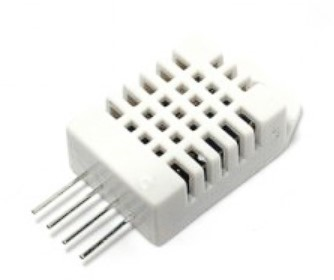
\includegraphics[width=.4\textwidth]{./Figures/DHT22.jpg}
	\caption{Fotografía del sensor DHT22\protect\footnotemark.}
	\label{fig:fotografiaDHT22}
\end{figure}

\footnotetext{Imagen tomada de \newline \url{https://www.openhacks.com/page/productos/id/84/title/Sensor-de-Humedad-y-Temperatura-DHT22}}

La elección del sensor DHT22 es debida a su mejor resolución y precisión frente a otros sensores, por ejemplo el DHT11 \citep{WEBSITE:DHT11}.


\subsection{Sensor de intensidad de luz}

El módulo Bh1750 \citep{WEBSITE:BH1750} es un sensor de intensidad de luz que esta compuesto por un conversor A/D (del inglés \textit{Analog to Digital}) \citep{WEBSITE:CONVERSORAD} de 16 bits. La principal ventaja del sensor es que brinda la intensidad luminosa en unidades de Lux.

La fotografía del sensor Bh1750 se presenta en la figura \ref{fig:fotografiaBh1750}.

\begin{figure}[H]
	\centering
	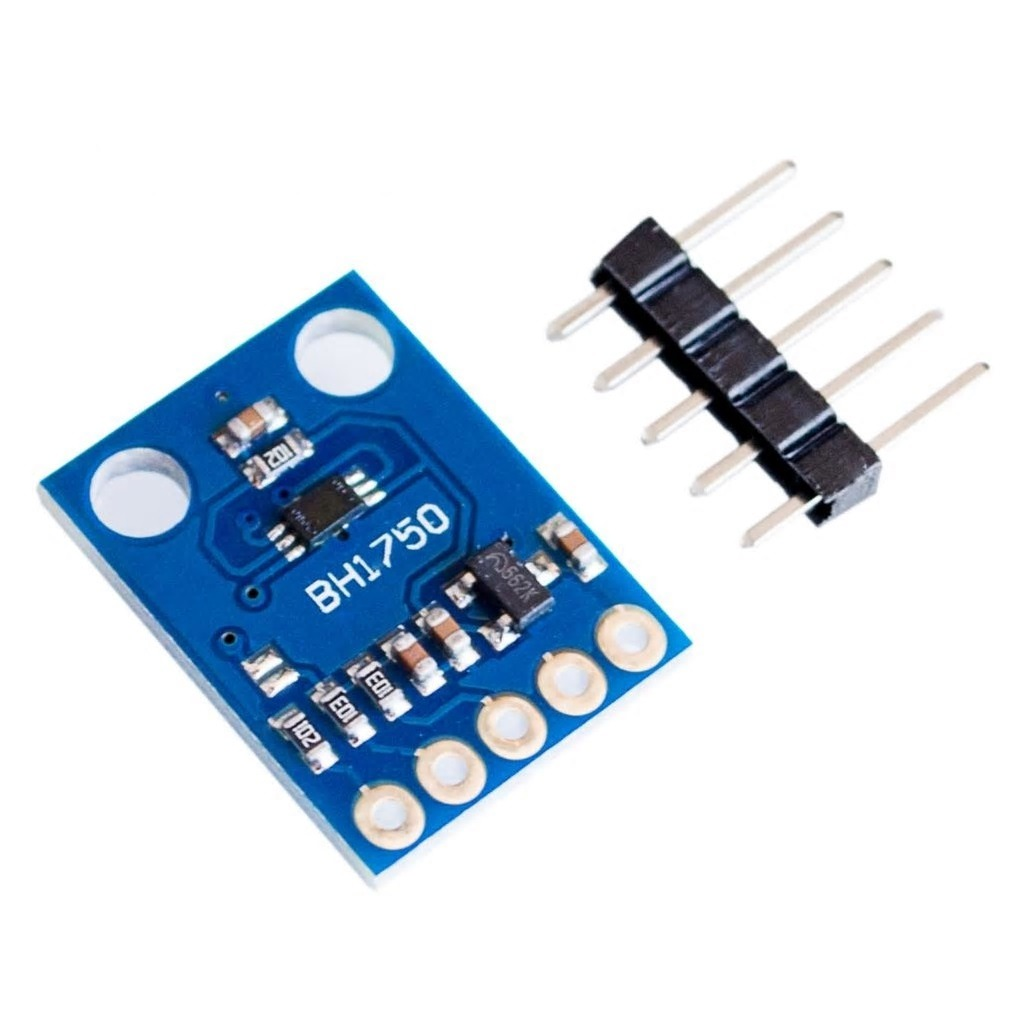
\includegraphics[width=.4\textwidth]{./Figures/Bh1750.jpg}
	\caption{Fotografía del sensor Bh1750\protect\footnotemark.}
	\label{fig:fotografiaBh1750}
\end{figure}

\footnotetext{Imagen tomada de \newline \url{https://candy-ho.com/producto/modulo-sensor-digital-luz-ambiente-lux-bh1750-arduino/}}

La elección del sensor Bh1750 es debida a su alta precisión y bajo costo en el mercado nacional. Otro factor importante en la decisión fue el poder brindar la intensidad de luz en Lux, sin necesidad de hacer alguna conversión.

\subsection{Sensor de calidad del aire}

El módulo MQ135 \citep{WEBSITE:MQ135} es un sensor de calidad del aire con alta sensibilidad al Amoníaco (NH3), óxidos de nitrógeno (NOx), alcohol, sulfuros, benceno (C6H6), CO2, humo y otros gases nocivos. Posee una salida analógica para indicar la concentración de gas en el ambiente y una digital que baja a 0 cuando la concentración de gas supera un nivel prefijado.

La fotografía del sensor MQ135 se presenta en la figura \ref{fig:fotografiaMQ135}.

\begin{figure}[H]
	\centering
	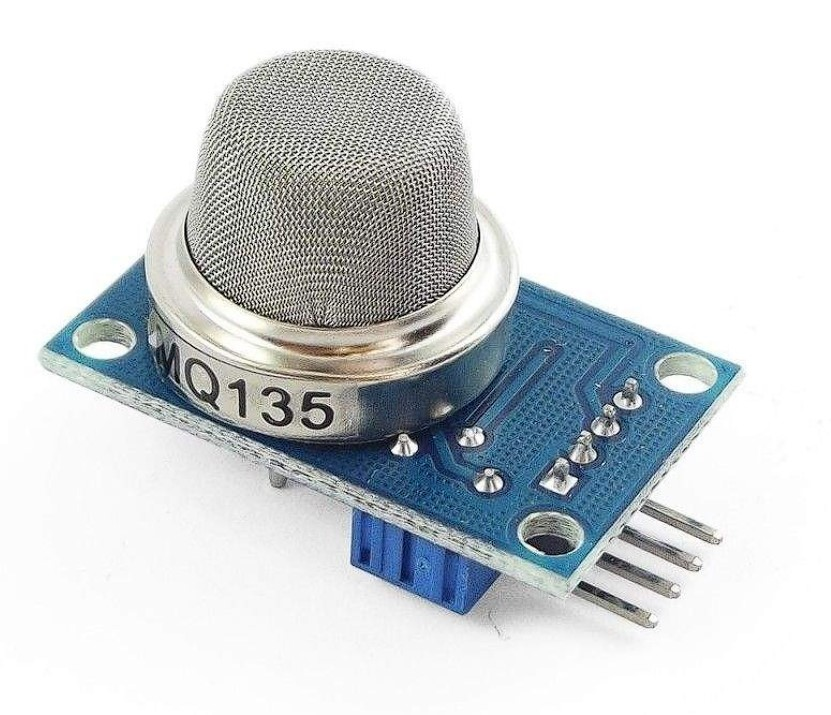
\includegraphics[width=.4\textwidth]{./Figures/MQ135.jpg}
	\caption{Fotografía del sensor MQ135\protect\footnotemark.}
	\label{fig:fotografiaMQ135}
\end{figure}

\footnotetext{Imagen tomada de \newline \url{https://www.micro-log.com/sensores-modulos-y-shields/3521-sensor-de-calidad-del-aire.html}}

La elección del sensor MQ135 es debida a su bajo costo y a la baja oferta de sensores similares en el mercado nacional.

\subsection{Sensor de flujo}

El módulo YF-S201B \citep{WEBSITE:YF-S201B} es un sensor de flujo que se utiliza para la medición de caudal o gasto volumétrico de un fluido en tuberías de 1/2” de diámetro.

Este sensor consiste en un cuerpo de válvula de plástico, un rotor y un sensor de efecto Hall \citep{WEBSITE:EFECTOHALL}. El rotor gira cuando el agua/líquido fluye a través de la válvula y su velocidad es directamente proporcional a la velocidad de flujo. El sensor de efecto Hall proporciona un impulso eléctrico con cada revolución del rotor. Este módulo sensor de flujo de agua puede ser fácilmente conectado con microcontroladores.

La fotografía del sensor YF-S201B se presenta en la figura \ref{fig:fotografiaYF-S201B}.

\begin{figure}[H]
	\centering
	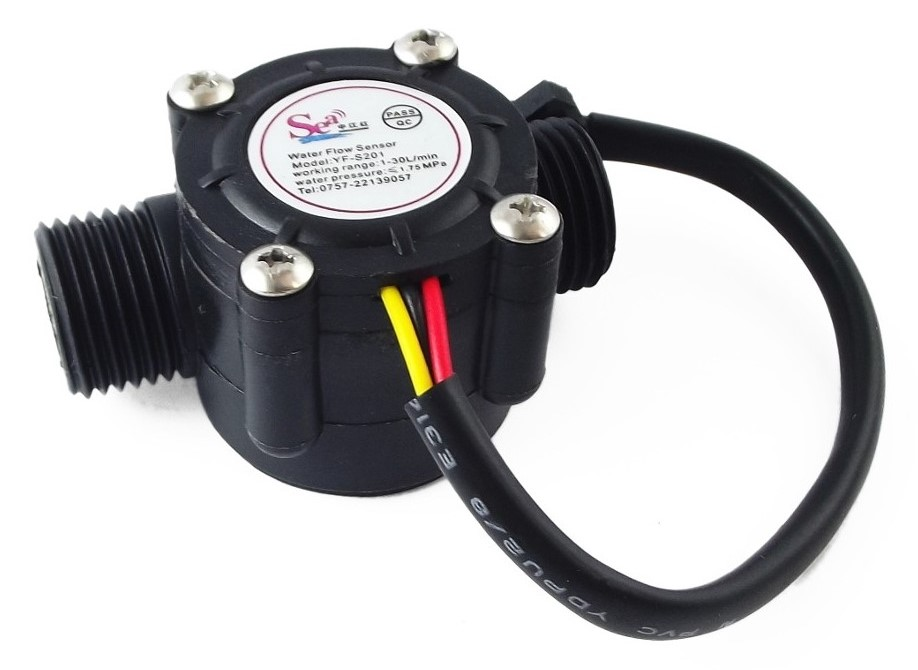
\includegraphics[width=.5\textwidth]{./Figures/YF-S201B.jpg}
	\caption{Fotografía del sensor YF-S201B\protect\footnotemark.}
	\label{fig:fotografiaYF-S201B}
\end{figure}

\footnotetext{Imagen tomada de \newline \url{https://naylampmechatronics.com/sensores-liquido/108-sensor-de-flujo-de-agua-12-yf-s201.html}}

La elección del sensor YF-S201B es debida a su bajo costo en el mercado nacional. Otros factores influyentes en la decisión fueron el bajo consumo y su facilidad de uso respecto a otros sensores similares.

\subsection{Sensor digital de temperatura para líquidos}

El módulo DS18B20 \citep{WEBSITE:DS18B20} sumergible es un sensor digital de temperatura que utiliza el protocolo 1-Wire \citep{WEBSITE:1WIRE} para comunicarse, el cual necesita solo un pin de datos y permite conectar más de un sensor en el mismo bus. La temperatura de funcionamiento es desde los -55 °C hasta los 125 °C y con una resolución programable desde 9 hasta 12 bits.

La fotografía del sensor DS18B20 sumergible se presenta en la figura \ref{fig:fotografiaDS18B20}.

\begin{figure}[H]
	\centering
	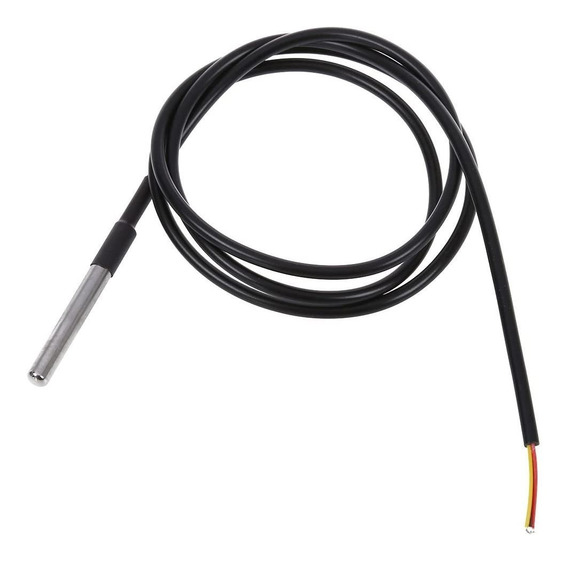
\includegraphics[width=.5\textwidth]{./Figures/DS18B20.jpg}
	\caption{Fotografía del sensor DS18B20 sumergible\protect\footnotemark.}
	\label{fig:fotografiaDS18B20}
\end{figure}

\footnotetext{Imagen tomada de \url{https://www.hobbytronica.com.ar/mla-903024959-ds18b20}}

La elección del sensor DS18B20 es debida a su facilidad de uso y amplio rango de medición.

\subsection{Módulo de \emph{relay}}

El \textit{relay} es un interruptor eléctrico para controlar el flujo de corriente. Puede estar cerrado o abierto con lo que permite o impide la circulación respectivamente.

La fotografía del módulo de \emph{relay} se presenta en la figura \ref{fig:fotografiaRelay}.

\begin{figure}[H]
	\centering
	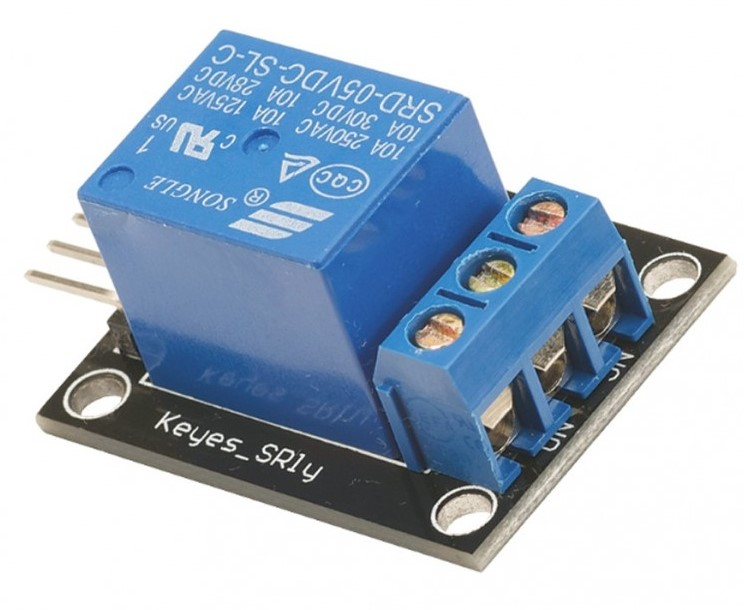
\includegraphics[width=.4\textwidth]{./Figures/Relay.jpg}
	\caption{Fotografía del módulo de \emph{relay}\protect\footnotemark.}
	\label{fig:fotografiaRelay}
\end{figure}

\footnotetext{Imagen tomada de \url{https://candy-ho.com/producto/modulo-rele-5v}}

La elección de incorporar un módulo de \emph{relay} es debida a que se quiere ofrecer al usuario del sistema un mecanismo para accionar dispositivos externos.

\section{Herramientas de \emph{software}}

\subsection{\textit{Progressive Web Apps}}

Las PWA (del inglés \textit{Progressive Web Apps}) \citep{WEBSITE:PWA} son aplicaciones web que utilizan APIs y funciones emergentes del navegador web junto a una estrategia tradicional de mejora progresiva para ofrecer una aplicación nativa. 

Para poder llamar PWA a una aplicación web, debe tener las siguientes características: uso de HTTPS, uno o más \emph{service workers} \citep{WEBSITE:SERVICEWORKERS} y un archivo de manifiesto \citep{WEBSITE:MANIFEST}.

Mediante los \emph{service workers} y otras tecnologías, las PWA pueden seguir ejecutándose en segundo plano sin tener que vivir dentro del navegador. Además, pueden instalarse en celulares y computadoras.

En la tabla \ref{tab:tablaComparacionAplicaciones} se puede observar una comparación entre aplicaciones nativas, aplicaciones web y PWA.

\begin{table}[h]
	\centering
	\caption[Comparación entre distintos tipos de aplicaciones]{Comparación entre distintos tipos de aplicaciones.}
	\begin{tabular}{l c c c}    
		\toprule
		\textbf{Descripción} & \textbf{Web} & \textbf{Nativa} & \textbf{PWA}\\
		\midrule
		Instalable & No & Sí & Sí \\	
		Multiplataforma & Sí & No & Sí \\	
		Notificaciones \emph{push} & No & Sí & Sí \\	
		Uso sin Internet & No & Sí & Sí \\	
		Diseño \emph{responsive} \citep{WEBSITE:RESPONSIVE} & Sí & Sí & Sí \\	
		Acceso al GPS & No & Sí & Sí \\
		\bottomrule
		\hline
	\end{tabular}
	\label{tab:tablaComparacionAplicaciones}
\end{table}

\subsection{\emph{Framework} del \emph{frontend}}

Angular \citep{WEBSITE:ANGULAR} es un \emph{framework} \citep{WEBSITE:FRAMEWORK} para aplicaciones web desarrollado en TypeScript \citep{WEBSITE:TYPESCRIPT}. Es de código abierto y mantenido por Google y se utiliza para crear y mantener aplicaciones web de una sola página \citep{WEBSITE:SPA}. Su objetivo es aumentar las aplicaciones basadas en navegador con capacidad de MVC (del inglés \textit{Model-View-Controller}) \citep{WEBSITE:MVC}, en un esfuerzo para hacer que el desarrollo y las pruebas sean más fáciles.

La biblioteca lee el HTML que contiene atributos de las etiquetas personalizadas adicionales, entonces obedece a las directivas de los atributos personalizados y une las piezas de entrada o salida de la página a un modelo representado por las variables estándar de JavaScript \citep{WEBSITE:JAVASCRIPT}.

Angular se basa en clases tipo componente, cuyas propiedades son las usadas para hacer el \emph{binding} de los datos. Dichas clases tienen propiedades y métodos.

La elección de Angular se debe a los siguientes factores: 
\begin{itemize}
	\item Posee alta escalabilidad.
	\item Al ser un \emph{framework} contiene muchas funcionalidades incorporadas, por ejemplo el manejo de rutas.
	\item Es fácil de adaptar a PWA.
	\item Tiene una documentación detallada.
	\item Posee una amplia variedad de bibliotecas disponibles.
	\item Tiene una comunidad activa.
\end{itemize}

En la tabla \ref{tab:tablaBibliotecasAngular} se pueden observar las bibliotecas de terceros utilizadas en la solución de Angular.

\begin{table}[h]
	\centering
	\caption[Bibliotecas de terceros utilizadas]{Bibliotecas de terceros utilizadas.}
	\begin{tabular}{l c c}    
		\toprule
		\textbf{Nombre} & \textbf{Descripción}\\
		\midrule
		@angular/material \citep{WEBSITE:ANGULARMATERIALLIBRARY} & Permite utilizar Material Design \citep{WEBSITE:ANGULARMATERIAL} \\	
		@swimlane/ngx-charts \citep{WEBSITE:NGXCHARTS} & Permite utilizar gráficos D3.js \citep{WEBSITE:D3JS} \\	
		socket.io-client \citep{WEBSITE:SOCKETIOCLIENT} & Permite utilizar Socket.IO \citep{WEBSITE:SOCKETIO} \\	
		ngx-cookieconsent \citep{WEBSITE:NGXCOOKIECONSENT} & \shortstack{Permite generar una alerta \\ del uso de cookies \citep{WEBSITE:COOKIES}} \\	
		ngx-countup \citep{WEBSITE:NGXCOUNTUP}& Permite generar animaciones numéricas \\	
		lite-server \citep{WEBSITE:LITESERVER}& \shortstack{Permite emular un despliegue \\ en un entorno local} \\	
		compression \citep{WEBSITE:COMPRESSIONLBIRARY} & Permite habilitar g-zip \citep{WEBSITE:GZIP} al usar lite-server \\	
		\bottomrule
		\hline
	\end{tabular}
	\label{tab:tablaBibliotecasAngular}
\end{table}

\subsection{Entorno en tiempo de ejecución del \emph{backend}}

Node.js \citep{WEBSITE:NODEJS} es un entorno de código abierto multiplataforma que ejecuta código JavaScript fuera de un navegador. Fue creado con el enfoque de ser útil en la creación de programas de red altamente escalables, como por ejemplo, servidores web.

La elección de Node.js se debe a los siguientes factores: 
\begin{itemize}
	\item Tiene la capacidad para manejar aplicaciones de alta concurrencia.
	\item Tiene la capacidad para escalar horizontalmente.
	\item Posee una amplia variedad de bibliotecas y paquetes disponibles.
	\item Brinda la posibilidad de usar TypeScript, tanto en el cliente como en el servidor.
	\item Tiene buen rendimiento.
	\item Tiene una comunidad activa.
\end{itemize}

En la tabla \ref{tab:tablaBibliotecasNodejs} se pueden observar las bibliotecas de terceros utilizadas en la solución de Node.js.

\begin{table}[H]
	\centering
	\caption[Bibliotecas de terceros utilizadas]{Bibliotecas de terceros utilizadas.}
	\begin{tabular}{l c c}    
		\toprule
		\textbf{Nombre} & \textbf{Descripción}\\
		\midrule
		bcryptjs \citep{WEBSITE:BCRYPTJS} & \shortstack{Permite realizar encriptaciones \citep{WEBSITE:ENCRIPTACION} \\ de contraseñas}\\	
		aedes \citep{WEBSITE:AEDES} & Permite generar un \emph{broker} MQTT \\	
		compression \citep{WEBSITE:COMPRESSIONLBIRARY} & Permite habilitar g-zip\\	
		cors \citep{WEBSITE:CORSLIBRARY} & Permite habilitar CORS \citep{WEBSITE:CORS} \\	
		dotenv \citep{WEBSITE:DOTENV} & \shortstack{Permite utilizar variables \\  de entorno \citep{WEBSITE:VARIABLESDEENTORNO}} \\	
		express \citep{WEBSITE:EXPRESSLIBRARY} & \shortstack{Permite utilizar el \\ \emph{framework} Express \citep{WEBSITE:EXPRESSJS}} \\	
		express-rate-limit \citep{WEBSITE:EXPRESSRATELIMIT} & \shortstack{Permite limitar la cantidad de \\ \textit{requests} permitidas} \\	
		jsonwebtoken \citep{WEBSITE:JSONWEBTOKENLIBRARY} & \shortstack{Permite utilizar \\ \emph{JSON Web Tokens} \citep{WEBSITE:JWT}} \\	
		mongoose \citep{WEBSITE:MONGOOSELIBRARY} & \shortstack{Permite utilizar el ORM \citep{WEBSITE:ORM} \\ mongoose \citep{WEBSITE:MONGOOSEJS}} \\	
		node-cron \citep{WEBSITE:NODECRON} & Permite programar tareas \\	
		nodemailer \citep{WEBSITE:NODEMAILER} & Permite enviar \textit{emails} \\	
		nodemailer-express-handlebars \citep{WEBSITE:NODEMAILEREXPRESSHANDLEBARS}& \shortstack{Permite agregar código \\ HTML a los \textit{emails}} \\	
		web-push \citep{WEBSITE:WEBPUSH} & Permite enviar notificaciones \emph{push}\\
		typescript \citep{WEBSITE:TYPESCRIPTLIBRARY} & Permite utilizar el lenguaje TypeScript \\
		nodemon \citep{WEBSITE:NODEMON} & \shortstack{Permite resetear automáticamente \\ el servidor si el código cambia} \\	
		supertest \citep{WEBSITE:SUPERTEST} & Permite probar servicios HTTP \\
		jest \citep{WEBSITE:JESTLIBRARY} & Permite el uso del \emph{framework} Jest \\
		ts-jest \citep{WEBSITE:TSJEST}& \shortstack{Permite usar TypeScript con \\ el \emph{framework} Jest} \\
		\bottomrule
		\hline
	\end{tabular}
	\label{tab:tablaBibliotecasNodejs}
\end{table}

\subsection{Base de datos}

MongoDB \citep{WEBSITE:MONGODB} es un sistema de base de datos NoSQL (del inglés \textit{Not Only Structured Query Language})\citep{WEBSITE:NOSQL}, orientado a documentos \citep{WEBSITE:BASEDEDATOSDOCUMENTAL} y de código abierto.

En lugar de guardar los datos en tablas, tal y como se hace en las bases de datos relacionales \citep{WEBSITE:BASEDEDATOSRELACIONAL}, MongoDB guarda estructuras de datos BSON (del inglés \textit{Binary JavaScript Object Notation}) \citep{WEBSITE:BSON} con un esquema dinámico, haciendo que la integración de los datos en ciertas aplicaciones sea más fácil y rápida. 

En la figura \ref{fig:ejemploDeModeladoDeDatosEnMongoDB} se presenta un ejemplo de modelado de datos en MongoDB, en el que puede observarse el formato de un documento BSON.

\begin{figure}[H]
	\centering
	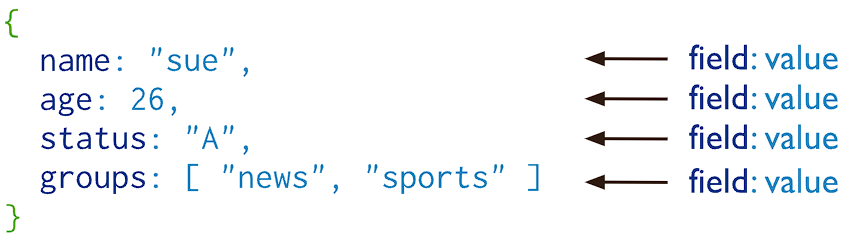
\includegraphics[width=.8\textwidth]{./Figures/Ejemplo de modelado de datos en MongoDB.png}
	\caption{Ejemplo de modelado de datos en MongoDB \protect\footnotemark.}
	\label{fig:ejemploDeModeladoDeDatosEnMongoDB}
\end{figure}

\footnotetext{Imagen tomada de \url{https://www.mongodb.com/docs/manual/core/document/}}

La elección de MongoDB se debe a los siguientes factores: 
\begin{itemize}
	\item Posee alta escalabilidad horizontal.
	\item Es altamente flexible en el modelo de datos.
	\item Tiene buen rendimiento.
	\item Es fácil de integrar con otras tecnologías.
	\item Tiene una comunidad activa.
\end{itemize}

\subsection{\emph{Framework} de pruebas del \emph{frontend}}

Jasmine \citep{WEBSITE:JASMINE} es un marco de pruebas de JavaScript diseñado para facilitar el desarrollo de pruebas automatizadas para aplicaciones web y aplicaciones escritas en JavaScript. Jasmine se basa en el patrón de pruebas BDD (del inglés \textit{Behavior-Driven Development}) \citep{WEBSITE:BDD} y se utiliza comúnmente para aplicaciones escritas en Angular.

Jasmine proporciona un conjunto de funciones y sintaxis para escribir pruebas que sean fáciles de leer y comprender.

La elección de Jasmine es debida a su integración incluida en Angular y a su velocidad de ejecución.

\subsection{\emph{Framework} de pruebas del \emph{backend}}

Jest \citep{WEBSITE:JESTJS} es un marco de pruebas de JavaScript desarrollado por Facebook. Al igual que Jasmine, Jest se utiliza para escribir y ejecutar pruebas automatizadas para aplicaciones web y aplicaciones escritas en JavaScript. Jest también se basa en el patrón de pruebas BDD y proporciona una sintaxis de prueba intuitiva y fácil de leer.

Jest se destaca por su velocidad de ejecución, que se debe en parte a su capacidad de realizar pruebas en paralelo y al uso de técnicas avanzadas de procesamiento en segundo plano. Jest también viene con una variedad de herramientas y utilidades para ayudar a los desarrolladores a escribir y ejecutar pruebas, incluyendo funciones de aserción para comparar valores, funciones  para configurar y limpiar el estado de las pruebas y utilidades para simular el comportamiento de objetos y funciones.

Además, Jest tiene una serie de características únicas, como la capacidad de realizar instantáneas \citep{WEBSITE:COPIAINSTANTANEA} de componentes de la interfaz de usuario y comprobarlos automáticamente para detectar cambios, así como la capacidad de integrarse con herramientas populares de automatización de tareas como Webpack \citep{WEBSITE:WEBPACK} y Babel \citep{WEBSITE:BABEL}. 

La elección de Jest se debe a los siguientes factores: 
\begin{itemize}
	\item Es fácil de usar.
	\item Es fácil de integrar con Node.js.
	\item Es rápido y eficiente.
	\item Tiene una función integrada para realizar cobertura de código.
	\item Tiene una gran comunidad activa.
\end{itemize}

\subsection{\emph{Software} de auditorías del \emph{frontend}}

Lighthouse \citep{WEBSITE:LIGHTHOUSE} es una herramienta automatizada de código abierto para mejorar la calidad de las páginas web. Se puede ejecutar contra cualquier página web pública o que requiera autenticación. Además, tiene auditorías de rendimiento, accesibilidad, PWA, mejores prácticas y SEO (del inglés \textit{Search Engine Optimization}).

En la figura \ref{fig:ejemploDeAuditoriaLighthouse} se presenta un ejemplo de una auditoría realizada con Lighthouse, en el que puede observarse las diferentes áreas que se evalúan.

\begin{figure}[H]
	\centering
	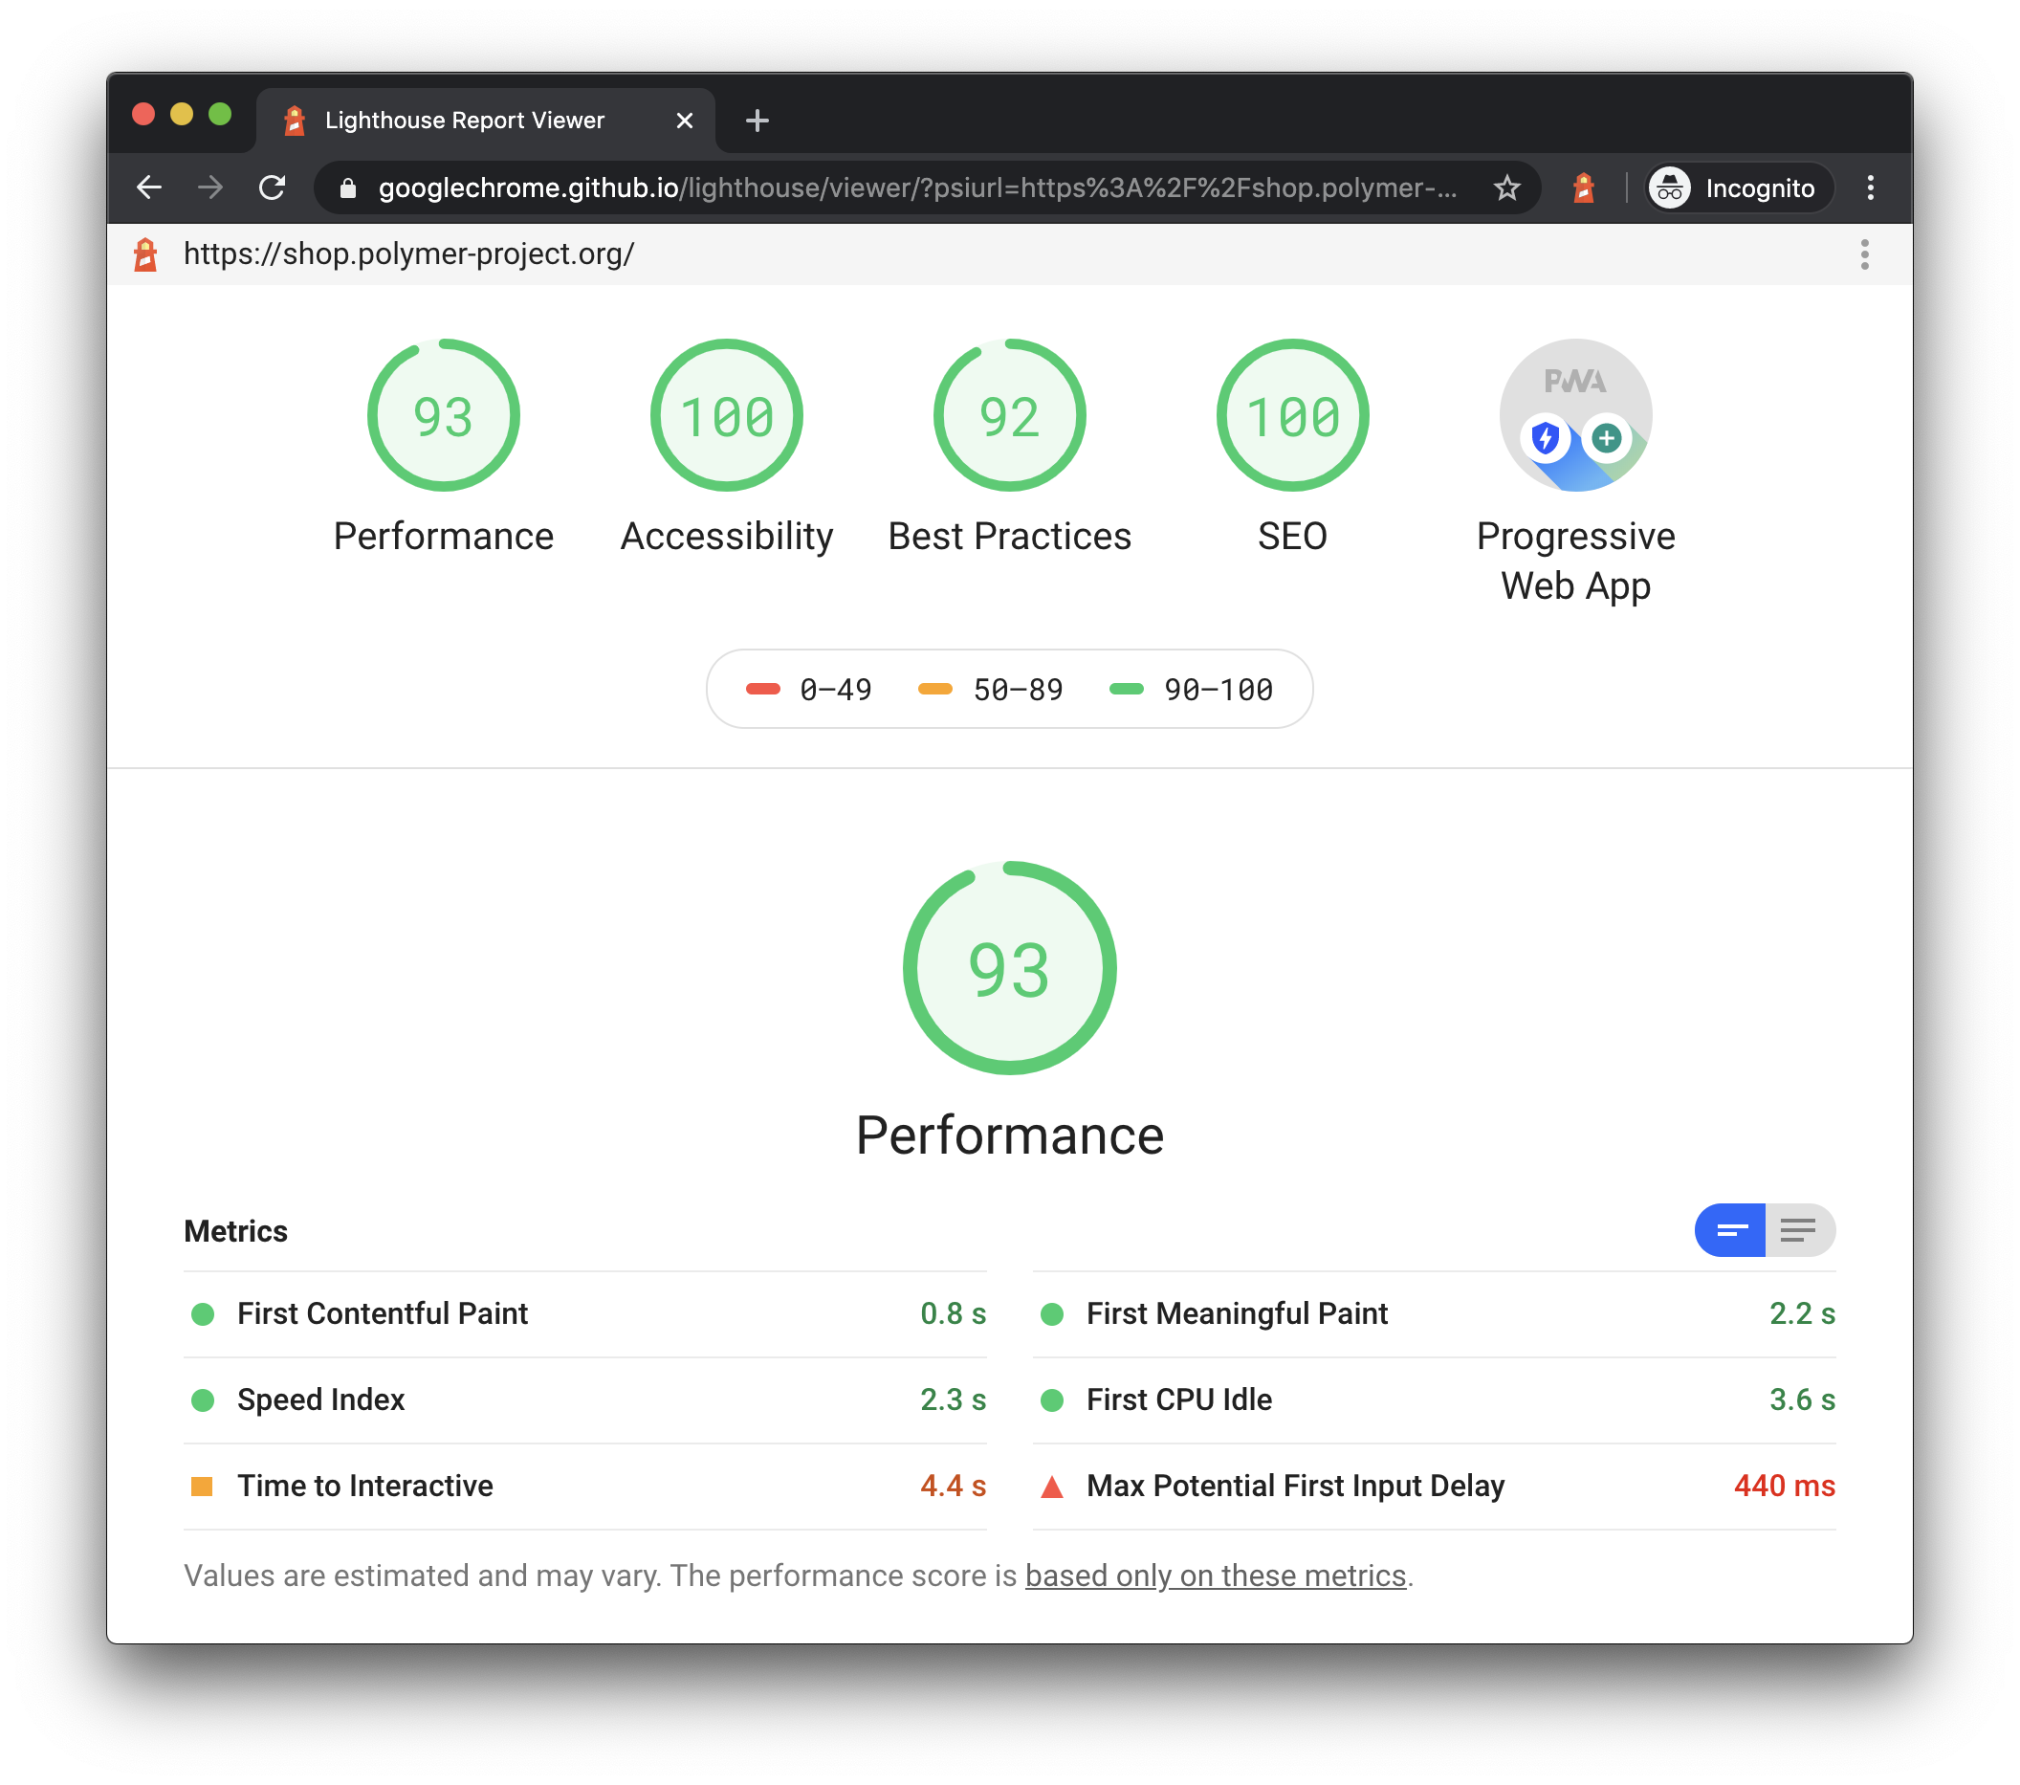
\includegraphics[width=.8\textwidth]{./Figures/Ejemplo de auditoria Lighthouse.png}
	\caption{Ejemplo de auditoría realizada en Lighthouse \protect\footnotemark.}
	\label{fig:ejemploDeAuditoriaLighthouse}
\end{figure}

\footnotetext{Imagen tomada de \url{https://es.semrush.com/blog/como-utilizar-google-lighthouse/}}

La elección de Lighthouse como herramienta de auditorías es debida a su integración incorporada en el navegador y sus pruebas extensivas en diferentes áreas. Otro factor influyente en la decisión fue que además de dar un amplio diagnóstico, también brinda posibles soluciones para cada uno de los problemas encontrados.
 
\chapter{Diseño e implementación} % Main chapter title

\label{Chapter3} % Change X to a consecutive number; for referencing this chapter elsewhere, use \ref{ChapterX}

En este capítulo se detallan los criterios de diseño que se tomaron para el desarrollo del sistema y los pasos seguidos para su implementación.

\definecolor{mygreen}{rgb}{0,0.6,0}
\definecolor{mygray}{rgb}{0.5,0.5,0.5}
\definecolor{mymauve}{rgb}{0.58,0,0.82}

%%%%%%%%%%%%%%%%%%%%%%%%%%%%%%%%%%%%%%%%%%%%%%%%%%%%%%%%%%%%%%%%%%%%%%%%%%%%%
% parámetros para configurar el formato del código en los entornos lstlisting
%%%%%%%%%%%%%%%%%%%%%%%%%%%%%%%%%%%%%%%%%%%%%%%%%%%%%%%%%%%%%%%%%%%%%%%%%%%%%
\lstset{ %
  backgroundcolor=\color{white},   % choose the background color; you must add \usepackage{color} or \usepackage{xcolor}
  basicstyle=\footnotesize,        % the size of the fonts that are used for the code
  breakatwhitespace=false,         % sets if automatic breaks should only happen at whitespace
  breaklines=true,                 % sets automatic line breaking
  captionpos=b,                    % sets the caption-position to bottom
  commentstyle=\color{mygreen},    % comment style
  deletekeywords={...},            % if you want to delete keywords from the given language
  %escapeinside={\%*}{*)},          % if you want to add LaTeX within your code
  %extendedchars=true,              % lets you use non-ASCII characters; for 8-bits encodings only, does not work with UTF-8
  %frame=single,	                % adds a frame around the code
  keepspaces=true,                 % keeps spaces in text, useful for keeping indentation of code (possibly needs columns=flexible)
  keywordstyle=\color{blue},       % keyword style
  language=[ANSI]C,                % the language of the code
  %otherkeywords={*,...},           % if you want to add more keywords to the set
  numbers=left,                    % where to put the line-numbers; possible values are (none, left, right)
  numbersep=5pt,                   % how far the line-numbers are from the code
  numberstyle=\tiny\color{mygray}, % the style that is used for the line-numbers
  rulecolor=\color{black},         % if not set, the frame-color may be changed on line-breaks within not-black text (e.g. comments (green here))
  showspaces=false,                % show spaces everywhere adding particular underscores; it overrides 'showstringspaces'
  showstringspaces=false,          % underline spaces within strings only
  showtabs=false,                  % show tabs within strings adding particular underscores
  stepnumber=1,                    % the step between two line-numbers. If it's 1, each line will be numbered
  stringstyle=\color{mymauve},     % string literal style
  tabsize=2,	                   % sets default tabsize to 2 spaces
  title=\lstname,                  % show the filename of files included with \lstinputlisting; also try caption instead of title
  morecomment=[s]{/*}{*/}
}


%----------------------------------------------------------------------------------------
%	SECTION 1
%----------------------------------------------------------------------------------------
\section{Arquitectura del sistema}

Una instalación está dividida en diferentes zonas de cultivos y en cada una se instala un microcontrolador ESP32 que se conecta usando MQTT con el \textit{broker} Aedes \citep{WEBSITE:AEDES}. En un sentido se envía la información de los sensores y en el otro los comandos para controlar los actuadores. El diagrama de la solución puede verse en la figura \ref{fig:diagramaEnBloques}.

El broker se encarga de autenticar y autorizar al microcontrolador. Una vez hecho esto, debe analizar la información recibida, validarla y en caso de ser necesario enviarla al DaaS de MongoDB para que sea almacenada. Además, el \textit{broker} por medio del protocolo WebSocket puede envíar los datos en tiempo real a la PWA. El servidor y el DaaS son compartidos entre todos los usuarios del sistema.

La API REST gestiona el acceso a los datos almacenados en el DaaS por medio de sus \textit{endpoints}. Estos últimos son ejecutados por la PWA por medio de HTTPS.

Por último, la PWA permite al usuario interactuar con el sistema por medio de sus interfaces.

Es importante destacar que todas las conexiones realizadas entre los componentes del sistema utilizan TLS para garantizar la seguridad en la comunicación. Además, todos los certificados TLS utilizados en el trabajo fueron generados mediante la herramienta openssl \citep{WEBSITE:OPENSSL} y se utilizó como DNS la IP de la computadora en la que se ejecutan los proyectos.

\begin{figure}[H]
	\centering
	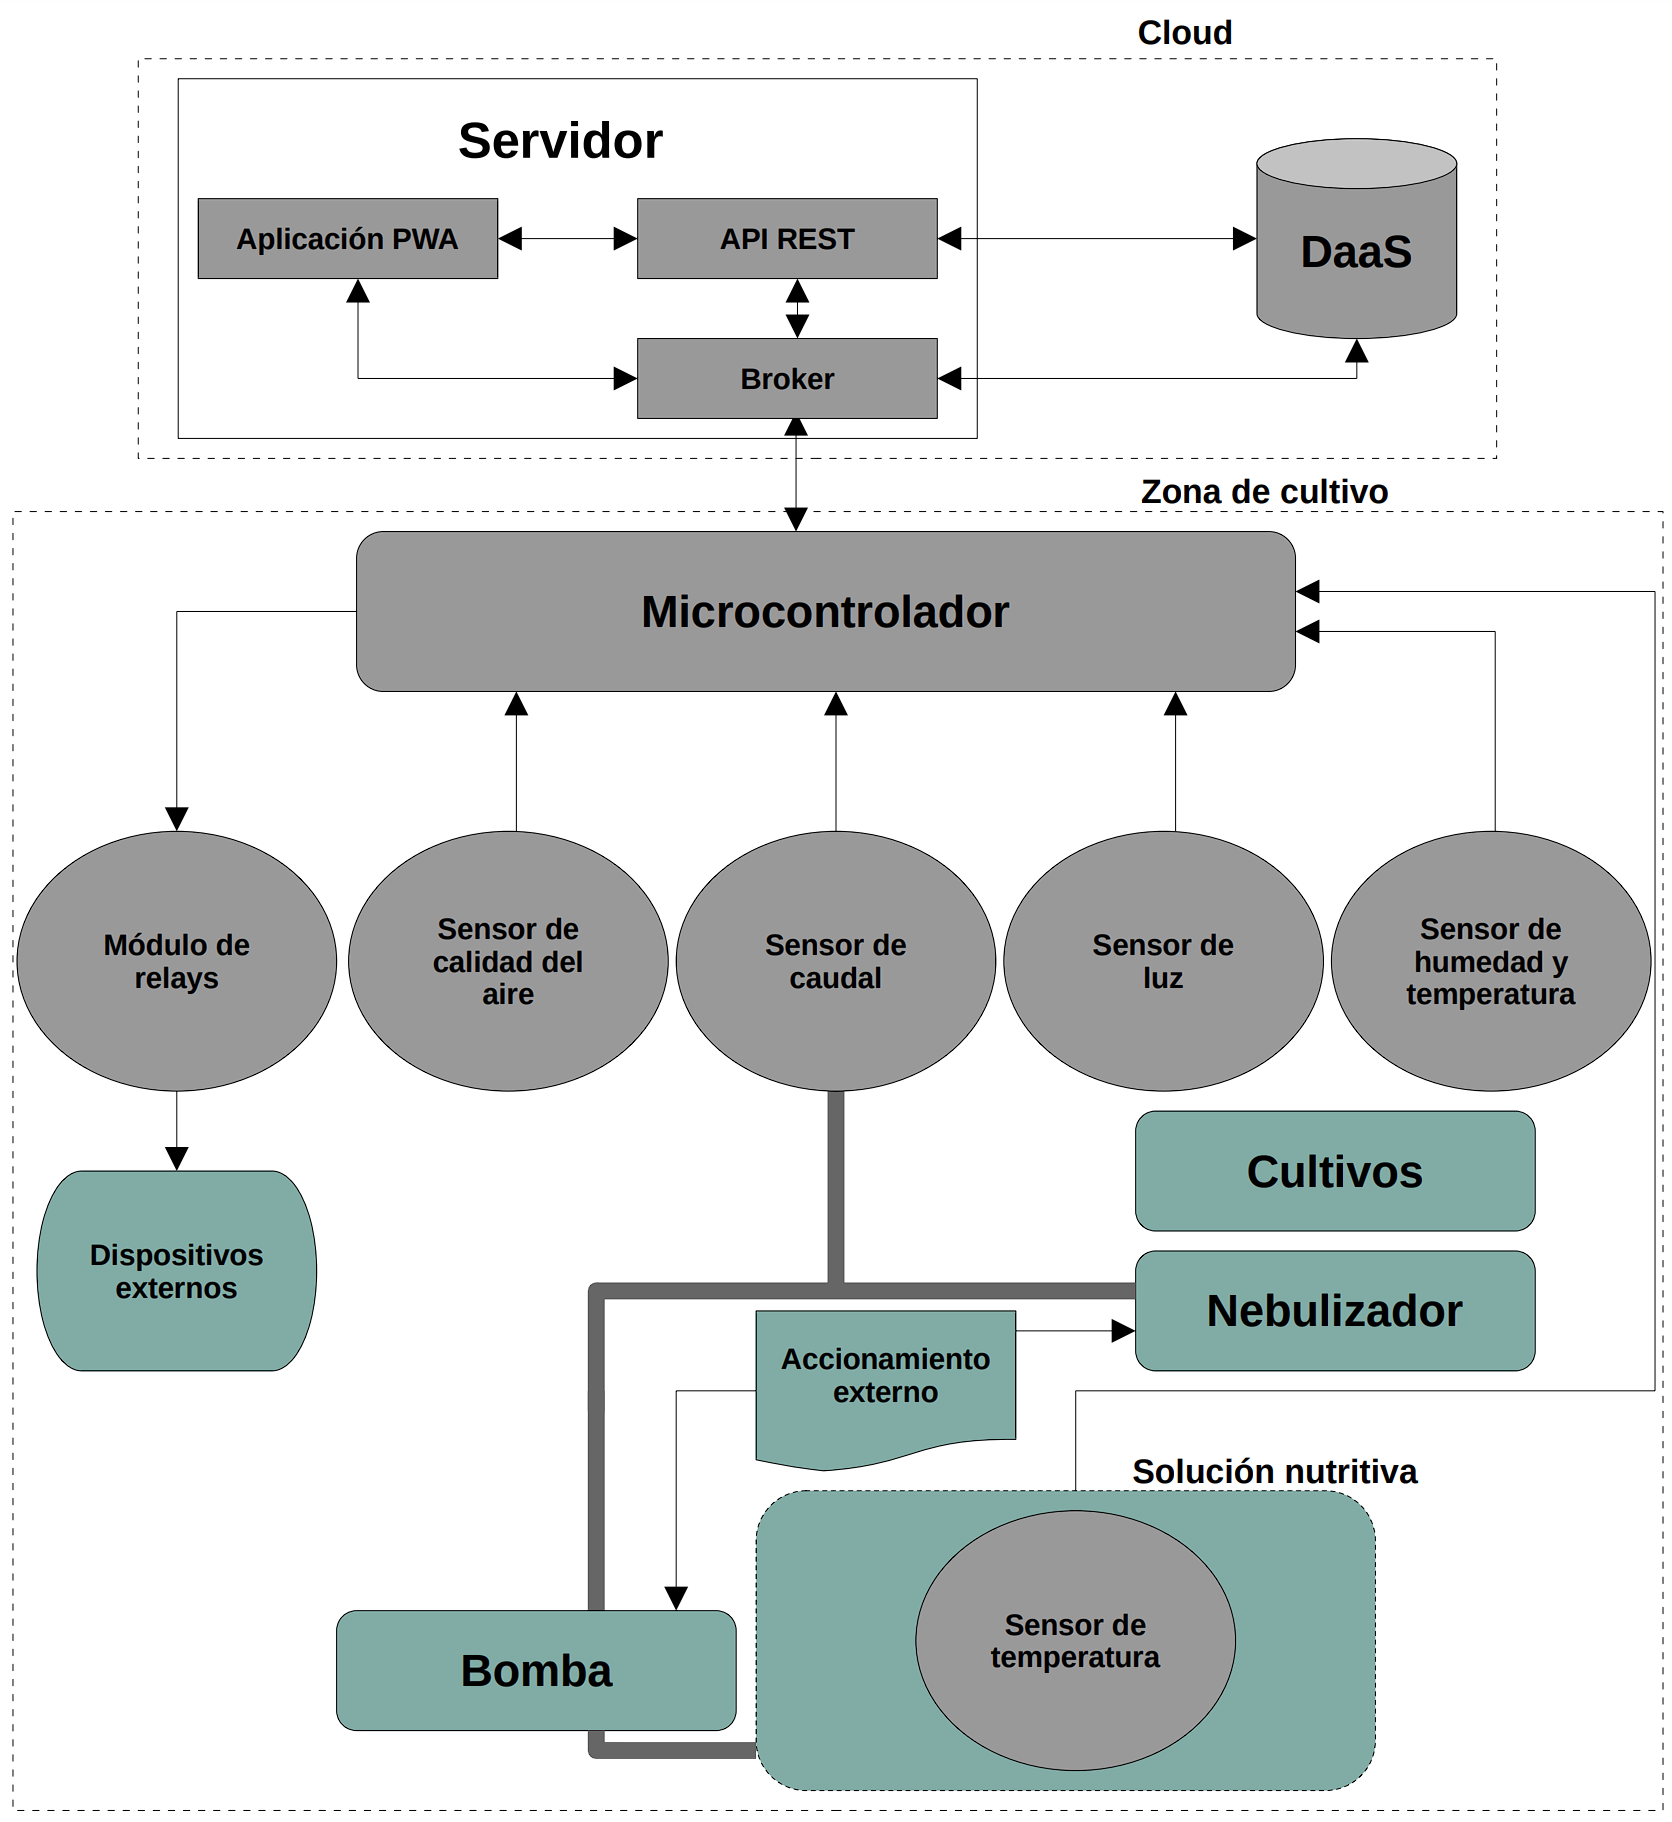
\includegraphics[width=1.00\textwidth]{./Figures/Diagrama en bloques v10.png}
	\caption{Diagrama en bloques de la solución.}
	\label{fig:diagramaEnBloques}
\end{figure}

\subsection{Observaciones}
\label{sec:observaciones}

Inicialmente, en la planificación del trabajo se había planteado utilizar una aplicación SSR. Sin embargo, a la hora de comenzar el desarrollo del \textit{frontend} se decidió que una PWA sería más adecuada, ya que otorga la posibilidad de usar ciertas funcionalidades que son útiles para el sistema,  por ejemplo tener un \emph{assets cache}, utilizar notificaciones \emph{push} y permitir instalar la aplicación en los dispositivos del usuario. 

También se realizaron modificaciones en los datos a almacenar en el DaaS para cada una de las colecciones con el fin de optimizar las consultas.

Estos cambios mencionados generaron modificaciones en algunos requerimientos y tareas del trabajo.

\section{Modelo de datos}

En esta sección se describen las diferentes colecciones que se almacenan en la base de datos de MongoDB. Con el objetivo de brindar una representación visual de las mismas, se presenta su estructura por medio de las interfaces utilizadas en la API REST.

\subsection{Colección \textit{Users}}

Es la colección que contiene los datos de los usuarios. Se presenta su estructura en la figura \ref{fig:coleccionUsers}. El campo \textit{verified} sirve para indicar si el usuario verificó su \textit{email}. La propiedad \textit{passwordHash} almacena el \emph{hash} de la contraseña. El atributo \textit{pushSubscription} es un objeto embebido dentro del documento y permite enviar notificaciones \emph{push} al usuario. 

\begin{figure}[H]
	\centering
	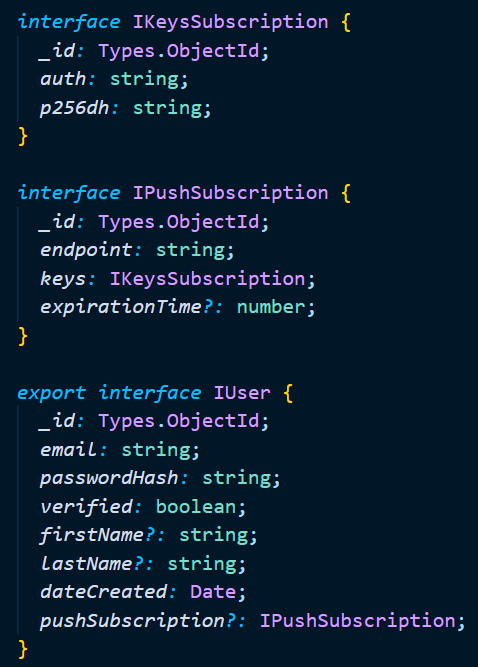
\includegraphics[width=.5\textwidth]{./Figures/Coleccion Users.png}
	\caption{Interface de la colección \textit{Users}.}
	\label{fig:coleccionUsers}
\end{figure}

\subsection{Colección \textit{Zones}}

Es la colección que contiene los datos de las zonas de cultivo. Se presenta su estructura en la figura \ref{fig:coleccionZones}. Los campos \textit{user} y \textit{lastMeasurement} son identificadores para hacer referencia a un documento de la colección \textit{Users} y \textit{Measurements}. El atributo \textit{device} es un objeto embebido dentro del documento. Este último tendrá las propiedades que indican el nombre, \emph{hash} de la contraseña, identificador de zona, identificador de usuario, alarmas asignadas junto con sus acciones automatizadas, \emph{relays} asignados y configuración de las notificaciones.

\begin{figure}[H]
	\centering
	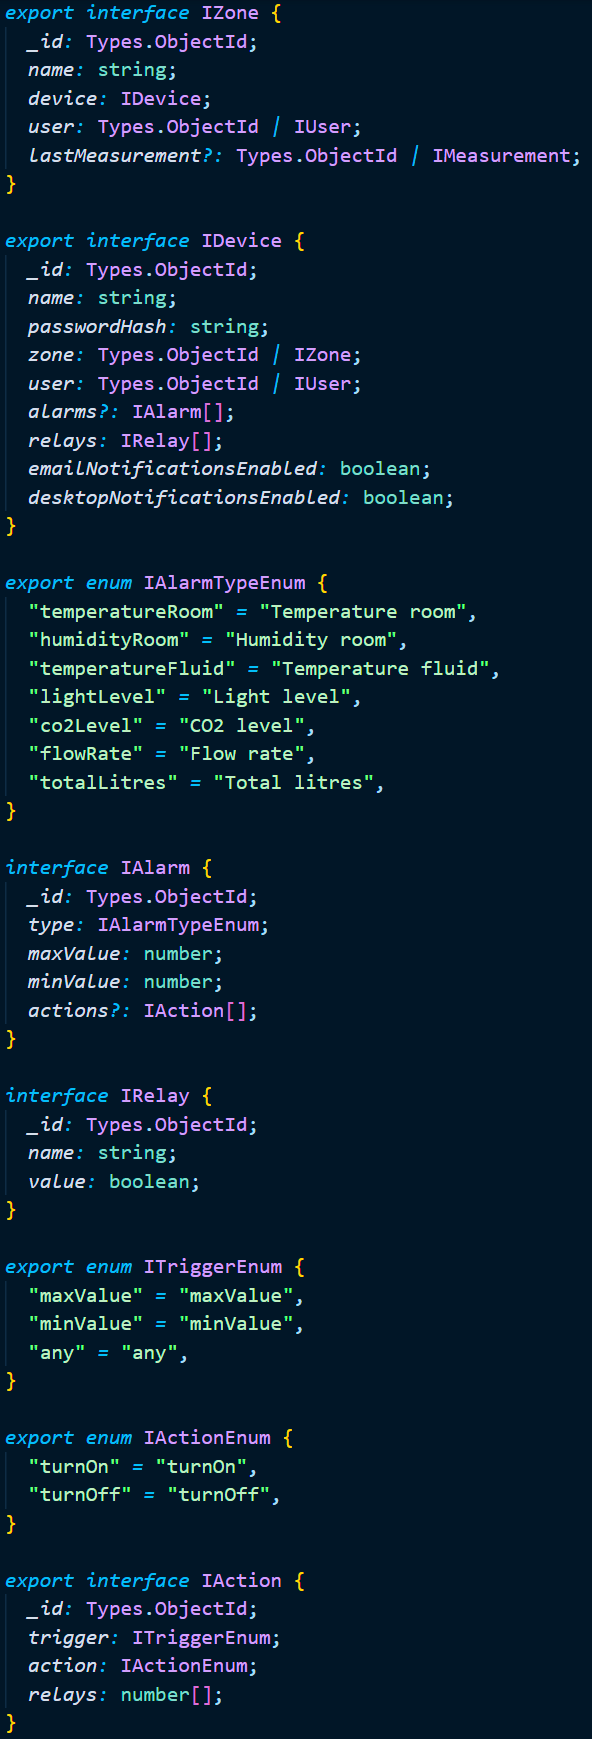
\includegraphics[width=.6\textwidth]{./Figures/Coleccion Zones.png}
	\caption{Interface de la colección \textit{Zones}.}
	\label{fig:coleccionZones}
\end{figure}

\subsection{Colección \textit{Notifications}}

Es la colección que contiene los datos de las notificaciones de los usuarios. Se presenta su estructura en la figura \ref{fig:coleccionNotifications}. Los campos \textit{zone}, \textit{device} y \textit{user} son identificadores para hacer referencia a un documento de la colección \textit{Zones}, \textit{Devices} y \textit{Users}. El atributo \textit{observation} almacena un mensaje que indica la condición que activó la alarma.

\begin{figure}[H]
	\centering
	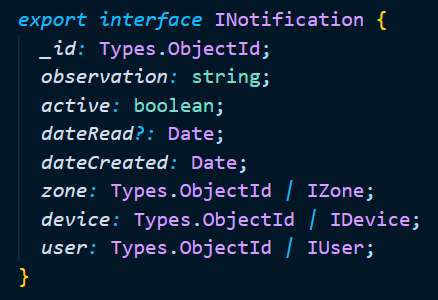
\includegraphics[width=.5\textwidth]{./Figures/Coleccion Notifications.png}
	\caption{Interface de la colección \textit{Notifications}.}
	\label{fig:coleccionNotifications}
\end{figure}

\subsection{Colección \textit{Measurements}}

Es la colección que contiene los datos de las mediciones de los sensores. Se presenta su estructura en la figura \ref{fig:coleccionMeasurements}. Las propiedades \textit{device}, \textit{zone} y \textit{user} son identificadores para hacer referencia a un documento de la colección \textit{Devices}, \textit{Zones} y \textit{Users}. El atributo \textit{timeReceived} contiene la fecha y hora de cuando se creó la medición.

\begin{figure}[H]
	\centering
	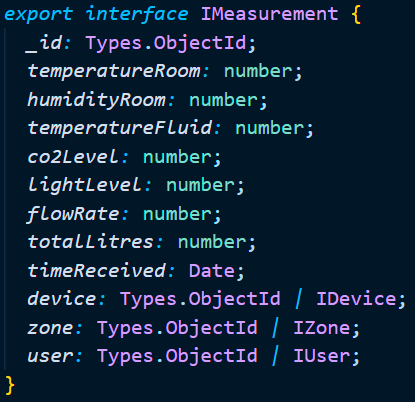
\includegraphics[width=.5\textwidth]{./Figures/Coleccion Measurements.png}
	\caption{Interface de la colección \textit{Measurements}.}
	\label{fig:coleccionMeasurements}
\end{figure}

\section{Desarrollo del \emph{backend}}

El \emph{backend} fue desarrollado en Node.js mediante TypeScript  y Express.

En el código \ref{cod:inicializacionBackend} se presenta la inicialización del \emph{backend} con certificados TLS. En las líneas 1 y 2 se obtienen los certificados. En las líneas 4 a 9 se crea el servidor con HTTPS con los certificados TLS.

\begin{lstlisting}[label=cod:inicializacionBackend,caption=Inicialización del \emph{backend} con TLS.]
const privateKey = readFileSync("./ssl/localhost.key");
const certificate = readFileSync("./ssl/localhost.crt");

const server = createServer(
   { key: privateKey, cert: certificate },
   app
).listen(port, () => {
   console.log(`[server]: Server is running at https://localhost:${port}`);
});
\end{lstlisting}

El \emph{backend} utiliza JWT (del inglés \textit{JSON Web Tokens}) para la autorización y autenticación de los usuarios. 

La autorización ocurre cuando un usuario inicia sesión en el sistema y el \emph{backend} le brinda un JWT firmado con una clave privada. En la figura \ref{fig:diagramaSecuenciaAutorizacionUsuarios} se visualiza un diagrama de secuencia del proceso.

\begin{figure}[H]
	\centering
	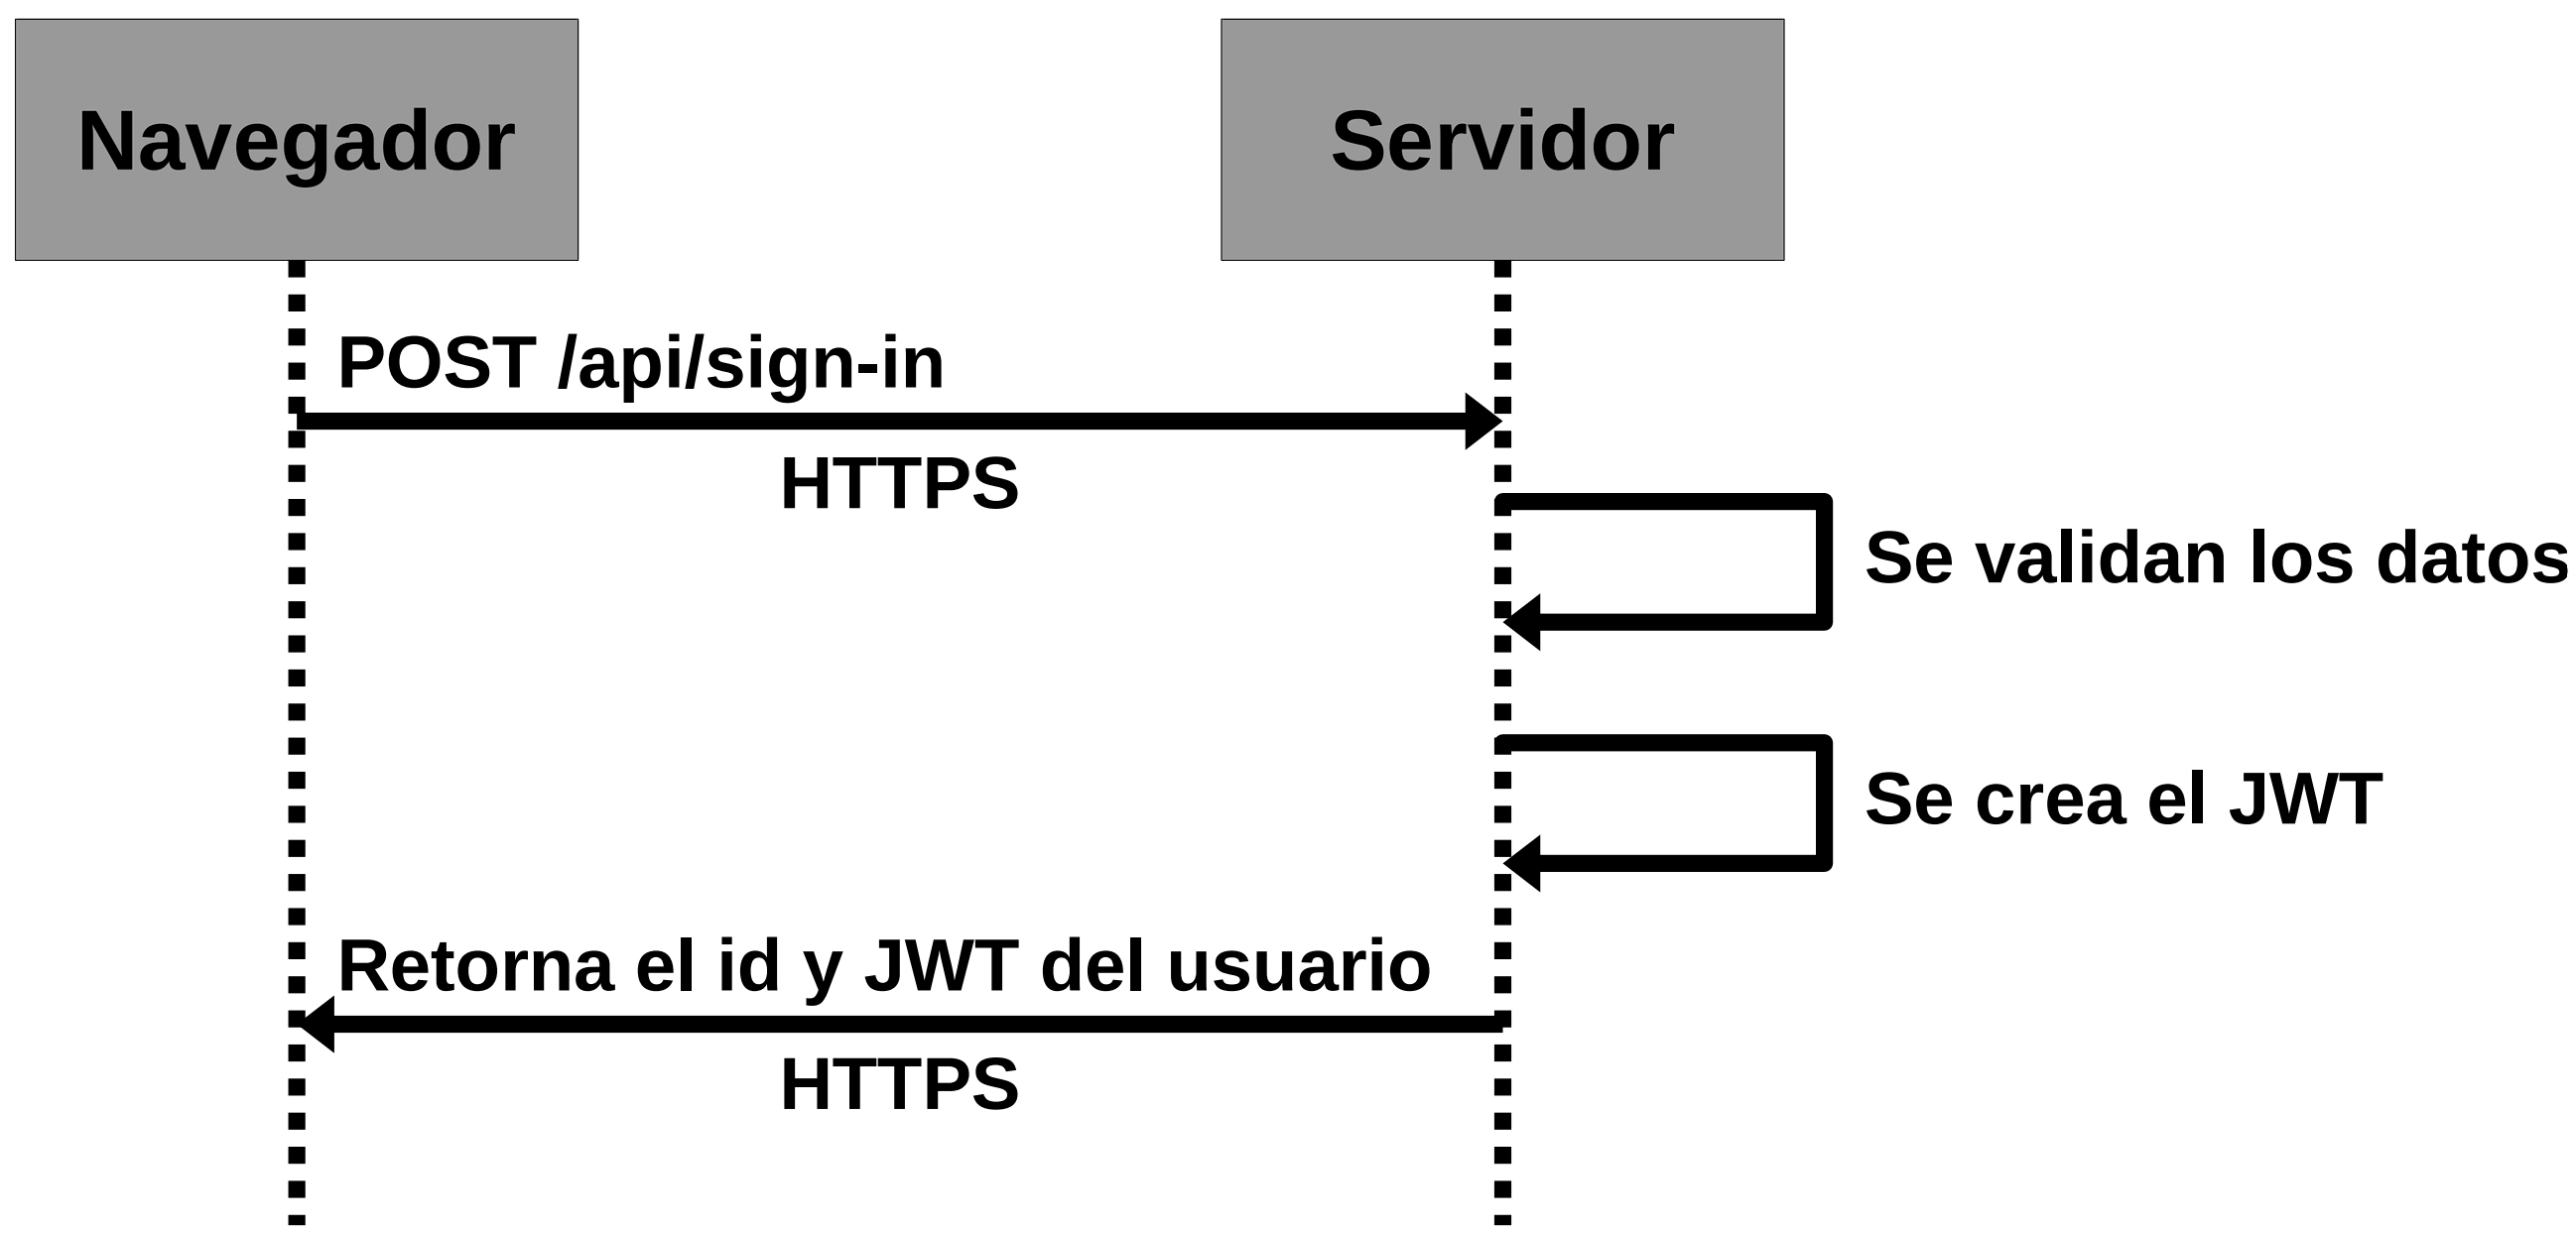
\includegraphics[width=.9\textwidth]{./Figures/Diagrama de secuencia autorizacion de usuarios.png}
	\caption{Diagrama de secuencia de la autorización de usuarios.}
	\label{fig:diagramaSecuenciaAutorizacionUsuarios}
\end{figure}

Si el usuario no dispone de credenciales válidas, la API responde con un código de error 400 y una breve descripción del error. Si se produce un error interno en el servidor, la API responde con un código de error 500.

En el código \ref{cod:autorizacionBackend} se presenta el proceso de autorización de los usuarios. En la línea 1 se obtiene la clave privada mediante las variables de entorno. En las líneas 6 a 8 se firma el \emph{payload} con la clave privada, también se asigna la expiración del JWT a siete días. En la línea 10 se le entrega al usuario el JWT junto con su id.

\begin{lstlisting}[label=cod:autorizacionBackend,caption=Autorización de usuarios.]
const accessTokenSecret = process.env["ACCESS_TOKEN_SECRET"] as string;
const payload = {
    _id: user._id,
    email: user.email,
};
const accessToken = jwt.sign(payload, accessTokenSecret, {
    expiresIn: "7d",
});

return response.status(200).json({ _id: user._id, accessToken });
\end{lstlisting} 

La autenticación ocurre cuando un usuario quiere acceder a un recurso protegido, por ejemplo un \emph{endpoint} y el \emph{backend} debe validar el JWT del usuario para determinar si puede acceder o no. En la figura \ref{fig:diagramaSecuenciaAutenticacionUsuarios} se visualiza un diagrama de secuencia del proceso.

\begin{figure}[H]
	\centering
	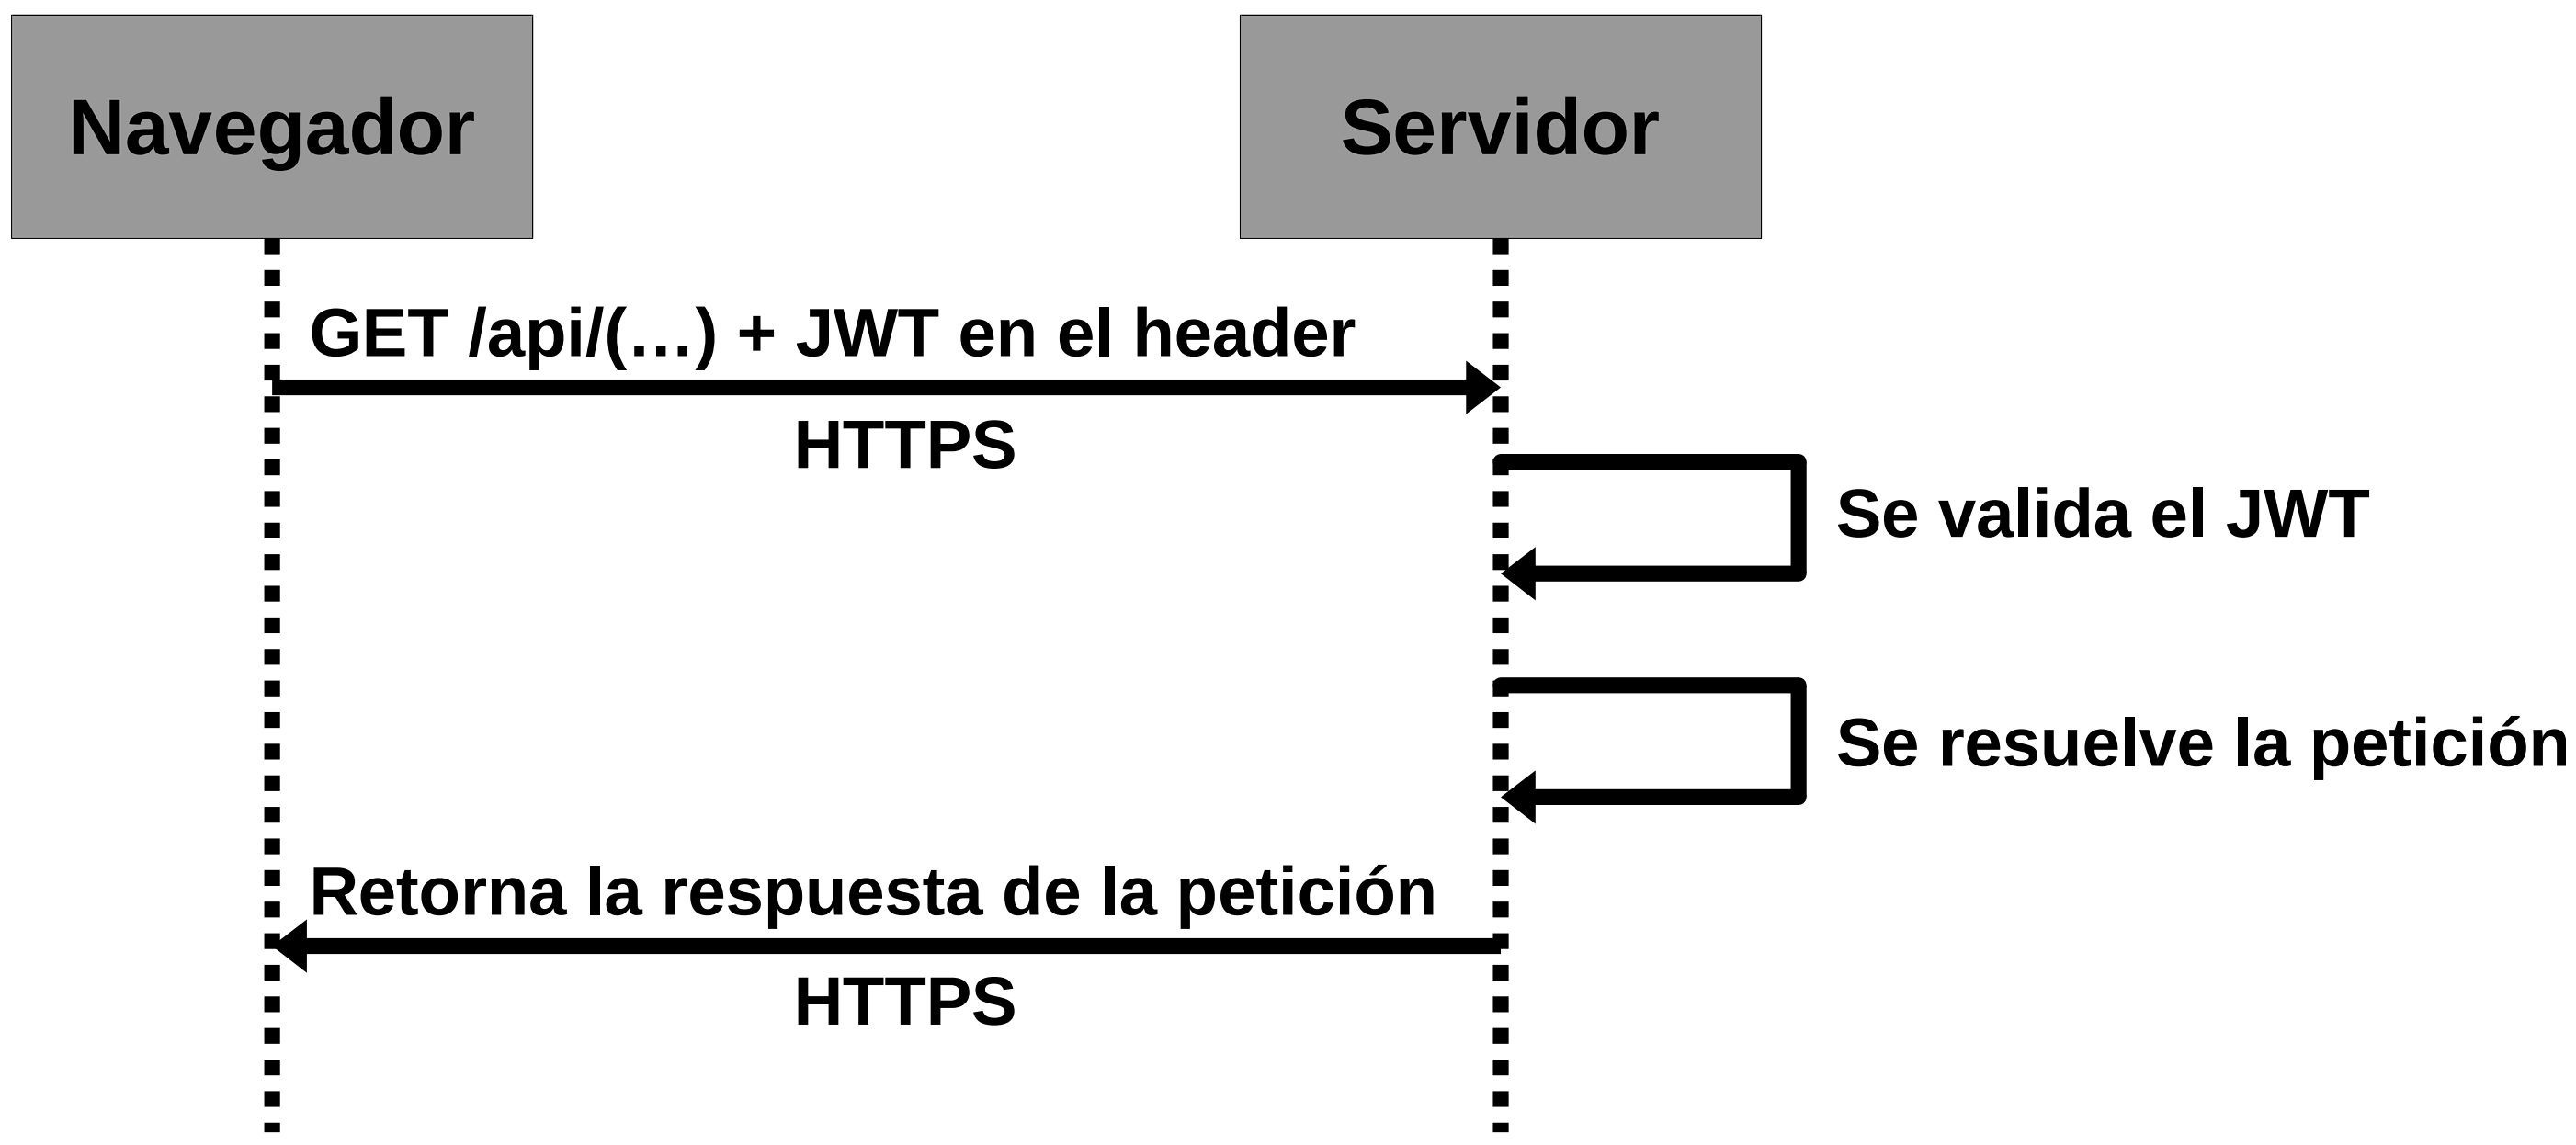
\includegraphics[width=.9\textwidth]{./Figures/Diagrama de secuencia autenticacion de usuarios.png}
	\caption{Diagrama de secuencia de la autenticación de usuarios.}
	\label{fig:diagramaSecuenciaAutenticacionUsuarios}
\end{figure}

Todos los \textit{endpoints} del sistema, excepto el de registro de usuarios y el de inicio de sesión, requieren el JWT del usuario para poder ser consultados. Si el usuario no envía el JWT, la API responde con un código de error 401. 

En el código \ref{cod:autenticaciónBackend} se presenta el proceso de autenticación de los usuarios mediante un \emph{middleware} que protege los \emph{endpoints}. En las líneas 6 a 11 se obtiene el JWT del \textit{authorization header} \citep{WEBSITE:HTTPHEADERAUTHORIZATION} de la \emph{request} y se valida que no sea nulo. En la línea 14 se verifica el JWT mediante la biblioteca jsonwebtoken. En las líneas 15 y 16 se guarda el id e \textit{email} del usuario en la respuesta HTTP.

\begin{lstlisting}[label=cod:autenticaciónBackend,caption=Autenticación de usuarios mediante un \emph{middleware}.]
export const authorization = (
  request: Request,
  response: Response,
  next: NextFunction
) => {
  const accessToken = request.headers.authorization?.split(" ")[1];
  const accessTokenSecret = process.env["ACCESS_TOKEN_SECRET"] as string;

  if (!accessToken) {
    return response.sendStatus(401);
  }

  try {
    const payloadData = verifyToken(accessToken, accessTokenSecret);
    response.locals._id = payloadData._id;
    response.locals.email = payloadData.email;

    return next();
  } catch {
    return response.sendStatus(401);
  }
};
\end{lstlisting}

En el código \ref{cod:endpointGetZonesBackend} se presenta un ejemplo de \emph{endpoint} que requiere la autenticación del usuario. En las líneas 1 y 2 se establece el nombre de la ruta junto con el método HTTP. En la línea 3 se aplica un \emph{middleware} a la ruta que verifica el \emph{token} del usuario. En la línea 6 se obtiene su id. En las líneas 7 a 9 se utiliza el ORM (del inglés \textit{Object-Relational-Mapping}) Mongoose para obtener las zonas que le pertenecen. En la línea 10 se le entrega una lista de sus zonas.

\begin{lstlisting}[label=cod:endpointGetZonesBackend,caption=\emph{Endpoint} que requiere autenticación.]
zoneRouter.get(
  "/",
  authorization,
  async (request: Request, response: Response) => {
    try {
      const userId = response.locals._id;
      const zones = await Zone.find({ user: userId })
        .populate("lastMeasurement")
        .exec();
      return response.status(200).json(zones);
    } catch (error) {
      return response.status(500).json(error);
    }
  }
);
\end{lstlisting} 

En la tabla \ref{tab:tablaEndpointsBackend} se pueden observar los \textit{endpoints} disponibles.

\begin{table}[H]
	\centering
	\caption[\textit{Endpoints} disponibles]{\textit{Endpoints} disponibles.}
	\begin{tabular}{l c c}    
		\toprule
		\textbf{\emph{Endpoint}} & \textbf{Método} & \textbf{Descripción}\\
		\midrule
		/auth/sign-up & \emph{POST} & \shortstack{Permite registrar un  \\ usuario} \\
		/auth/sign-in & \emph{POST} & Permite iniciar sesión \\
		/auth/verifyToken & \emph{GET} & Permite verificar al usuario \\
		/auth/profile & \emph{GET} & \shortstack{Permite obtener los \\ datos del usuario} \\
		/auth/profile & \emph{PATCH} & \shortstack{Permite actualizar los \\ datos del usuario} \\
		/notifications & \emph{GET} & \shortstack{Permite obtener las \\ notificaciones} \\
		/notifications/markAsRead/:id & \emph{PATCH} & \shortstack{Permite marcar una \\ notificación como leída } \\
		/notifications/subscribe & \emph{PATCH} & \shortstack{Permite suscribirse a \\ las notificaciones } \\
		/measurements/zones/id: & \emph{POST} & \shortstack{Permite simular una \\ medición en una zona} \\
		/measurements/zones/:id & \emph{GET} &  \shortstack{Permite obtener las \\ mediciones de una zona } \\
		/zones & \emph{GET} & \shortstack{Permite obtener las zonas } \\
		/zones/:id & \emph{GET} & Permite obtener una zona \\
		/zones & \emph{POST} & Permite crear una zona \\
		/zones & \emph{PATCH} & \shortstack{Permite actualizar los \\  datos de una zona } \\
		/zones/:id & \emph{DELETE} & Permite eliminar una zona \\
		/zones/relays/:id & \emph{PATCH} & \shortstack{Permite actualizar los \\  datos de un \emph{relay} } \\
		\bottomrule
		\hline
	\end{tabular}
	\label{tab:tablaEndpointsBackend}
\end{table}

En la figura \ref{fig:estructuraDeDirectoriosDelBackend} se presenta la estructura de directorios. La descripción de los contenidos de las carpetas y archivos relevantes es:
\begin{itemize}
	\item models: contiene las interfaces que permiten al ORM Mongoose tipificar las colecciones de MongoDB.
	\item routes: contiene los \emph{endpoints}.
	\item schemas: contiene los esquemas que permiten al ORM Mongoose crear las colecciones en MongoDB.
	\item ssl: contiene los certificados TLS.
	\item utils: contiene un \emph{middleware} para autorizar los \emph{endpoints} necesarios. Además, contiene funciones que se reutilizan en todo el proyecto.
	\item .env: contiene las variables de entorno.
	\item broker.ts: contiene la inicialización y configuración del \emph{broker} Aedes.
	\item index.ts: contiene la inicialización y configuración del \emph{backend}.
	\item jest.config.js: contiene la configuración de Jest.
	\item ts.config.json: contiene la configuración de TypeScript.
\end{itemize}

\begin{figure}[H]
	\centering
	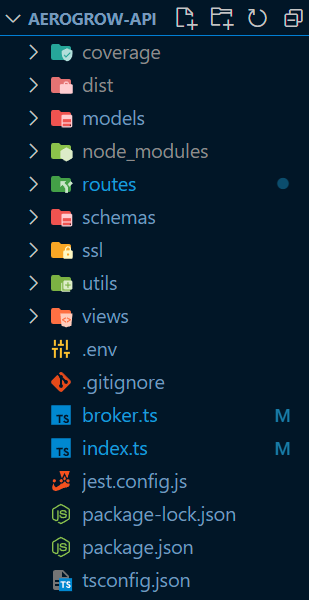
\includegraphics[width=.4\textwidth]{./Figures/Estructura de directorios del backend.png}
	\caption{Estructura de directorios.}
	\label{fig:estructuraDeDirectoriosDelBackend}
\end{figure}

\section{Desarrollo del \emph{frontend}}
El \emph{frontend} del trabajo fue desarrollado en TypeScript con Angular y como \textit{framework} de estilos se utilizó Angular Material.

La estrategia de diseño que se utilizó fue la de crear una PWA con un enfoque de diseño \emph{responsive} \citep{WEBSITE:RESPONSIVE}.

Para obtener el mejor rendimiento posible en la aplicación se aplicaron diferentes estrategias de optimización \citep{WEBSITE:ANGULAROPTIMIZACION1} \citep{WEBSITE:ANGULAROPTIMIZACION2}, entre ellas destacan las siguientes:
\begin{itemize}
	\item \emph{Lazy loading} de rutas.
	\item \emph{Lazy loading} de imágenes.
	\item Uso de \textit{ChangeDetectionStrategy.onPush} en los componentes.
	\item \textit{Assets cache}.
	\item Evitar llamadas de funciones en las vistas HTML.
	\item Utilizar el \emph{guard} canLoad.
	\item Evitar el uso de bibliotecas que no sean esenciales para el trabajo.
	\item Evitar suscripciones manuales a un \textit{Observable} \citep{WEBSITE:OBSERVABLE}. 
\end{itemize}

En la figura \ref{fig:certificadosTLSDelFrontend} se presenta la configuración para utilizar certificados TLS.

\begin{figure}[H]
	\centering
	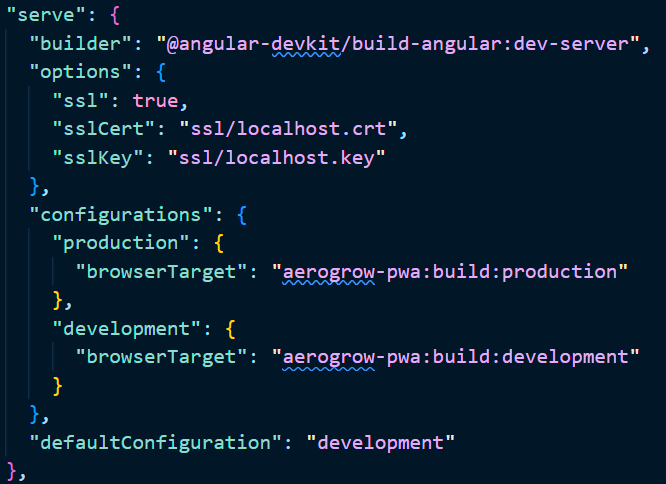
\includegraphics[width=.7\textwidth]{./Figures/Certificados TLS en Angular.png}
	\caption{Uso de certificados TLS.}
	\label{fig:certificadosTLSDelFrontend}
\end{figure}

La PWA utiliza un \emph{guard} para la autenticación de las rutas.  En el código \ref{cod:autenticaciónFrontend} se presenta el proceso de autenticación de las rutas. En la línea 7 se obtiene el estado de la sesión del usuario. En las líneas 9 a 13 se verifica su estado: si inició sesión puede entrar a la ruta, caso contrario se le redirecciona a la pantalla del \emph{login}.

\newpage
\begin{lstlisting}[label=cod:autenticaciónFrontend,caption=Autenticación de rutas.]
export const authGuard = (
  route: ActivatedRouteSnapshot,
  state: RouterStateSnapshot
) => {
  const router = inject(Router);
  const authService = inject(AuthService);
  const isLoggedIn = authService.isLoggedIn();

  return isLoggedIn
    ? true
    : router.navigate(['/sign-in'], {
        queryParams: { returnUrl: state.url },
      });
};
\end{lstlisting} 

En la tabla \ref{tab:tablaRutasFrontend} se pueden observar las rutas disponibles.

\begin{table}[H]
	\centering
	\caption[Rutas disponibles]{Rutas disponibles.}
	\begin{tabular}{l c c}    
		\toprule
		\textbf{Ruta}& \textbf{Descripción}\\
		\midrule
		/ & Pantalla de listado de zonas \\
		/profile & Pantalla de edición de un usuario \\
		/zones & Pantalla de listado de zonas \\
		/zones/create & Pantalla de creación de una zona \\
		/zones/edit/:id & Pantalla de edición de una zona \\
		/notifications & Pantalla de listado de notificaciones \\
		/dashboard/:id & Pantalla de \emph{dashboard} de una zona \\
		/sign-in & Pantalla de inicio de sesión \\
		/sign-up & Pantalla de registro de usuario \\
		/error/:code & Pantalla de manejo de errores \\
		\bottomrule
		\hline
	\end{tabular}
	\label{tab:tablaRutasFrontend}
\end{table}

En la figura \ref{fig:estructuraDeDirectoriosDelFrontend} se presenta la estructura de directorios. La descripción de los contenidos de las carpetas y archivos relevantes es:
\begin{itemize}
	\item src/app/components: contiene los componentes del proyecto.
	\item src/app/guards: contiene un \emph{guard} para autenticar las rutas.
	\item src/app/interceptors: contiene un \textit{interceptor} que añade el JWT del usuario al \textit{header} de la \emph{request} y gestiona los errores de las \emph{requests} HTTP.
	\item src/app/models: contiene las interfaces para tipificar los datos del sistema.
	\item src/app/services: contiene los servicios del proyecto.
	\item src/app/utils: contiene funciones que se reutilizan en todo el proyecto.
	\item src/app/app.component.ts: contiene el componente con el que se inicializa la aplicación.  
	\item src/app/routes.ts: contiene las rutas de la aplicación.
	\item src/assets: contiene los \emph{assets} del \emph{frontend}.
	\item src/manifest.webmanifest: contiene el archivo de manifiesto del proyecto.
	\item src/robots.txt: contiene la configuración para los \emph{crawlers} \citep{WEBSITE:CRAWLER}.
	\item angular.json: contiene la configuración de Angular.
	\item bs-config.js: contiene la configuración de lite-server. 
	\item karma.config: contiene la configuración de Jasmine y Karma \citep{WEBSITE:KARMA} para las pruebas.
	\item ngsw-config: contiene la configuración del \emph{service worker} de la PWA.
	\item ts.config.json: contiene la configuración de TypeScript.
\end{itemize}

\begin{figure}[H]
	\centering
	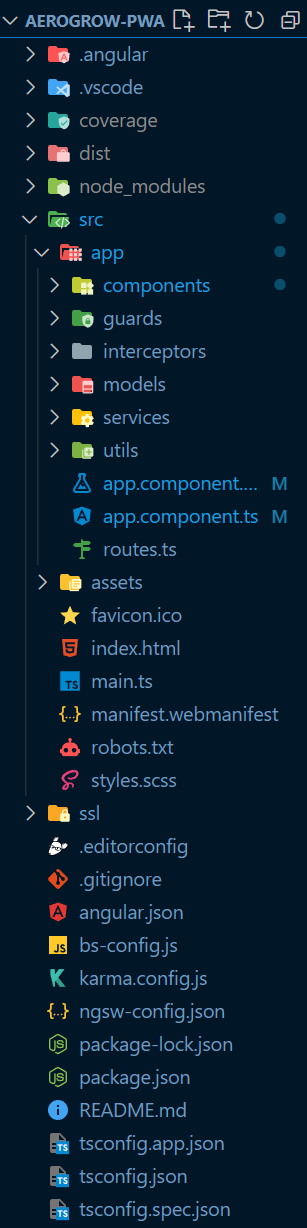
\includegraphics[width=.4\textwidth, height=1.35\linewidth]{./Figures/Estructura de directorios del frontend.png}
	\caption{Estructura de directorios.}
	\label{fig:estructuraDeDirectoriosDelFrontend}
\end{figure}

\subsection{Principales pantallas de la aplicación}

En la figura \ref{fig:formularioSignUp} se visualiza la pantalla de creación de usuarios. Para dar de alta un nuevo usuario se debe ingresar de forma mandatoria su  \textit{email} y contraseña, de forma opcional se puede agregar el nombre y apellido. Las cuentas tienen un lapso de 10 días para confirmarse mediante \textit{email} antes de ser eliminadas.

\begin{figure}[H]
	\centering
	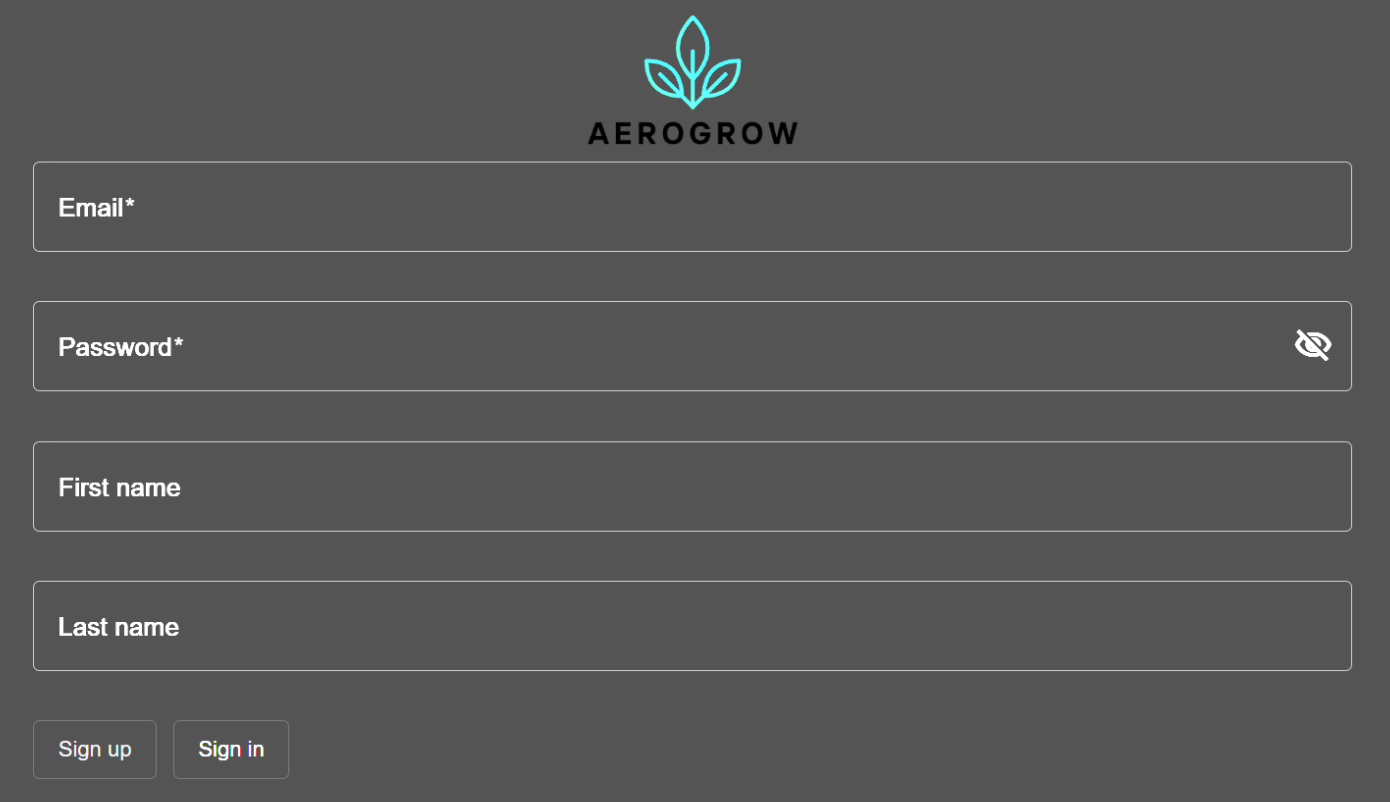
\includegraphics[width=.8\textwidth]{./Figures/Frontend formulario de creacion de nueva cuenta.png}
	\caption{Pantalla de registro de usuario.}
	\label{fig:formularioSignUp}
\end{figure}

En la figura \ref{fig:listaDeZonas} se visualiza la pantalla del listado de zonas de un usuario. Desde esta pantalla, puede realizar las siguientes acciones:

\begin{itemize}
	\item Acceder a una pantalla para crear una nueva zona.
	\item Acceder a una pantalla para editar una zona.
	\item Acceder a una pantalla \emph{dashboard} de una zona.
	\item Eliminar una zona.
	\item Monitorear en tiempo real todas las zonas listadas.
	\item Exportar los datos del listado en formato xlsx.
	\item Copiar las credenciales de una zona.
\end{itemize}

El listado de zonas se puede filtrar y ordenar por cualquiera de los campos de la tabla.

\begin{figure}[H]
	\centering
	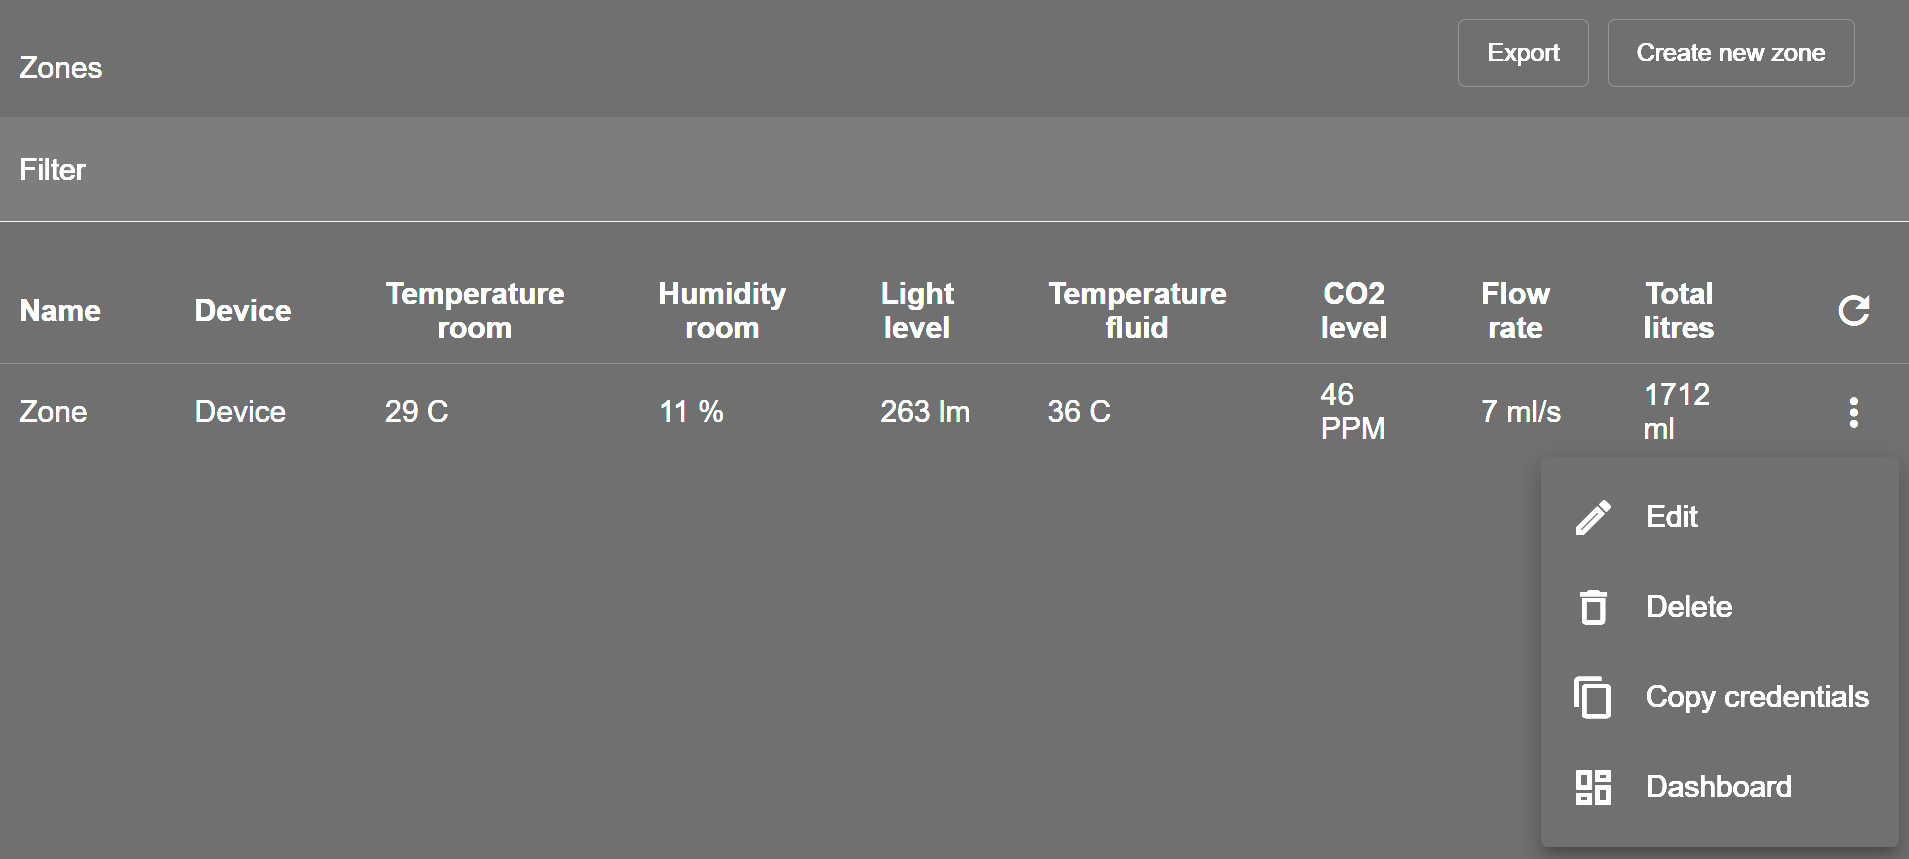
\includegraphics[width=.9\textwidth]{./Figures/Frontend lista de zonas.png}
	\caption{Pantalla de listado de zonas.}
	\label{fig:listaDeZonas}
\end{figure}

En la figura \ref{fig:formularioDeZona} se visualiza la pantalla de creación de zonas. Para crear una nueva zona se debe ingresar un nombre y también el nombre y contraseña del dispositivo. De manera opcional, se puede ingresar la configuración para las notificaciones, los \textit{relays} y alarmas asociadas al dispositivo y las acciones automatizadas a realizar en caso de que la alarma se dispare. El mismo componente es utilizado para la edición de zonas. 

\begin{figure}[H]
	\centering
	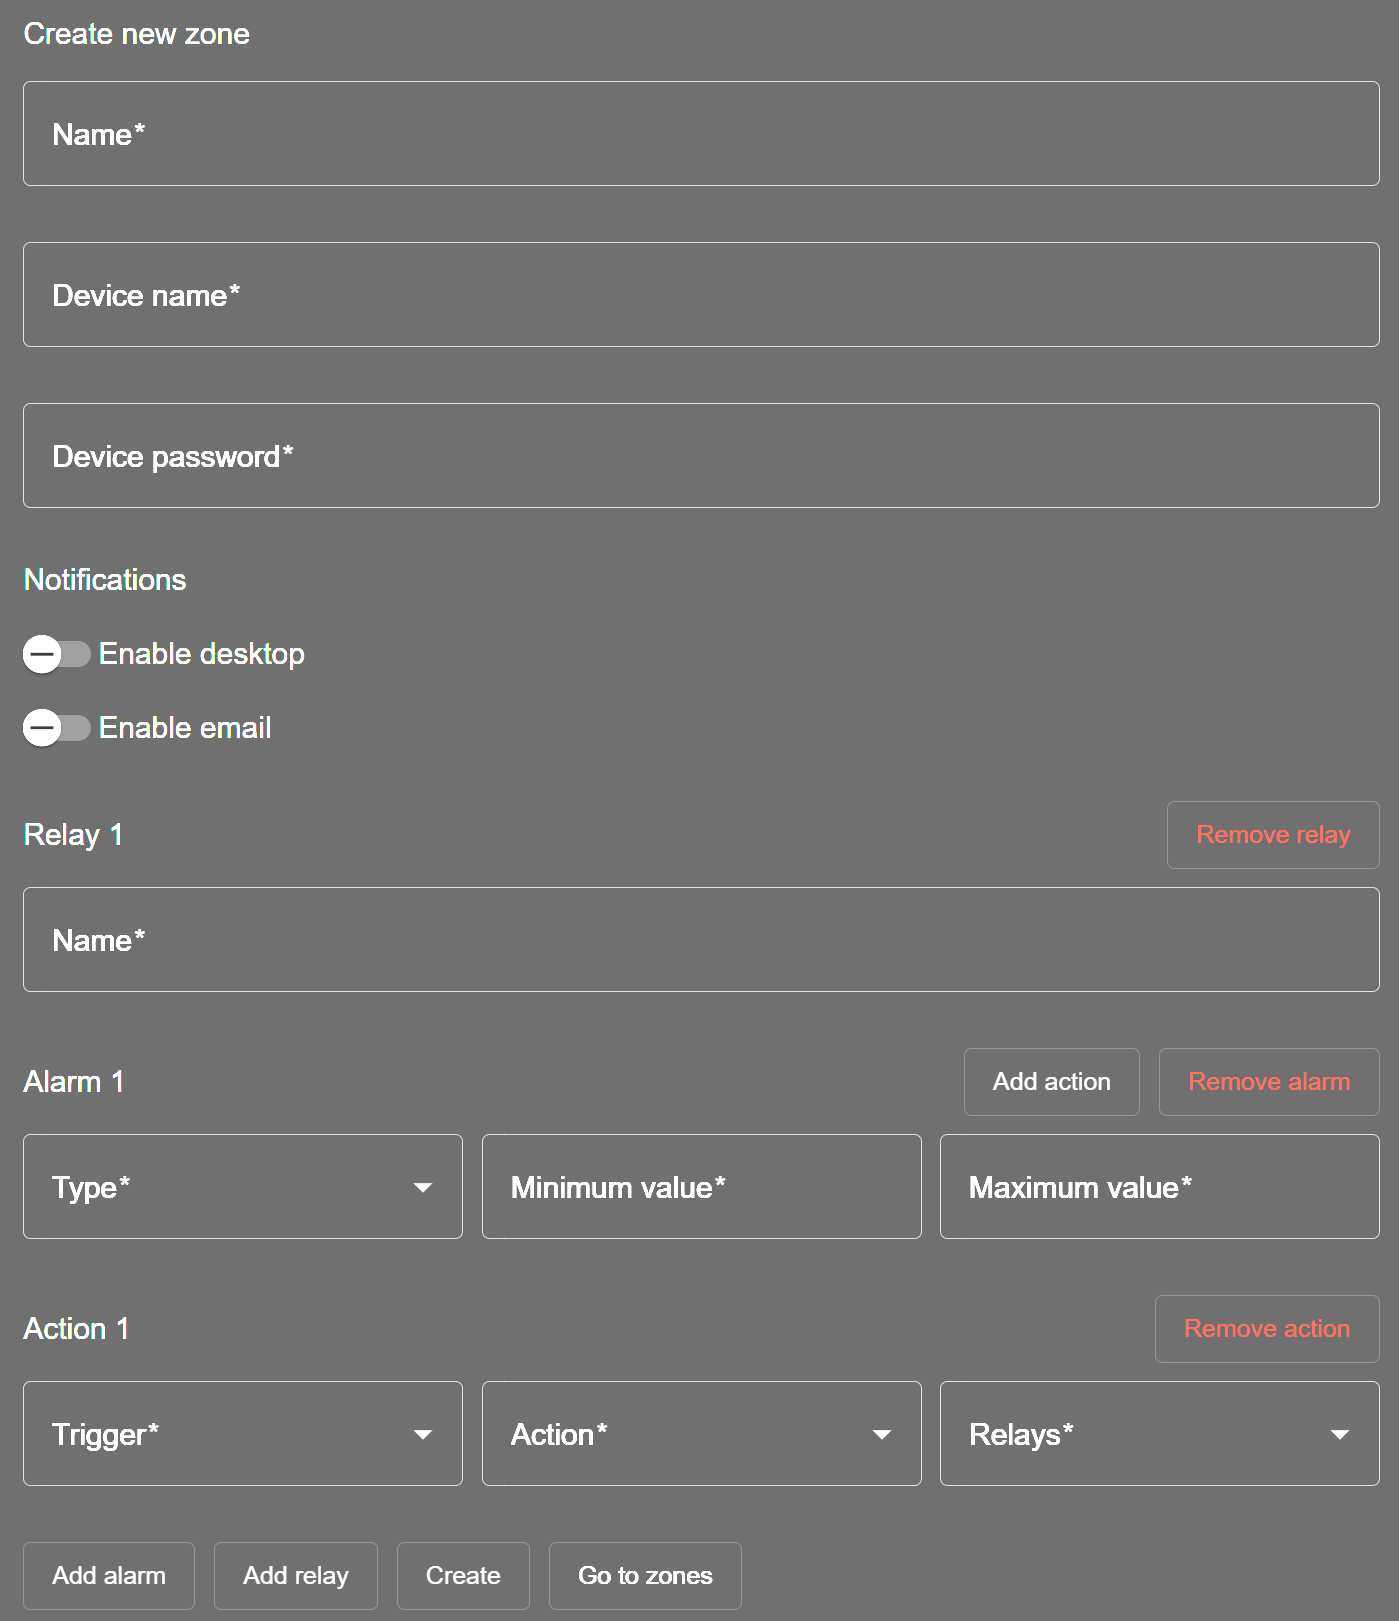
\includegraphics[width=.7\textwidth]{./Figures/Frontend formulario de zona.png}
	\caption{Pantalla de creación de una zona.}
	\label{fig:formularioDeZona}
\end{figure}

En la figura \ref{fig:notificacionAlarmaEmail} se visualiza un ejemplo de \textit{email} de notificación que envía el sistema. Este tipo de notificación se genera cuando una medición activa una alarma y las notificaciones de \textit{email} están habilitadas en la zona de cultivo.

\begin{figure}[H]
	\centering
	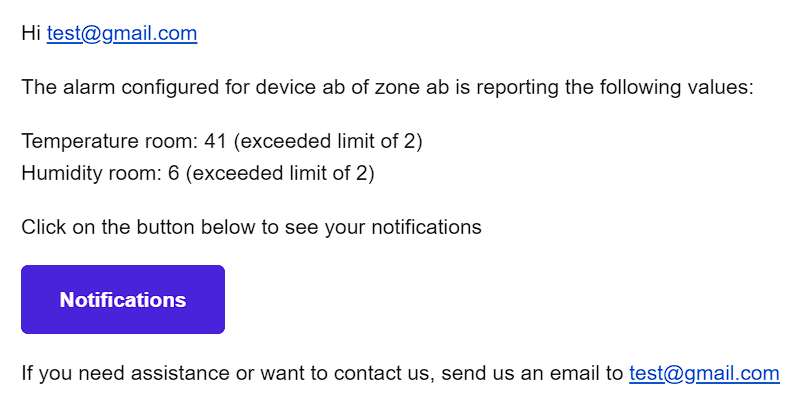
\includegraphics[width=.8\textwidth]{./Figures/Notificacion email.png}
	\caption{Ejemplo de \textit{email} de notificación de alarma.}
	\label{fig:notificacionAlarmaEmail}
\end{figure}

En la figura \ref{fig:notificacionPushEmail} se visualiza un ejemplo de notificación \emph{push} que envía el sistema. Este tipo de notificación se genera cuando una medición activa una alarma y las notificaciones de escritorio están habilitadas en la zona de cultivo.

\begin{figure}[H]
	\centering
	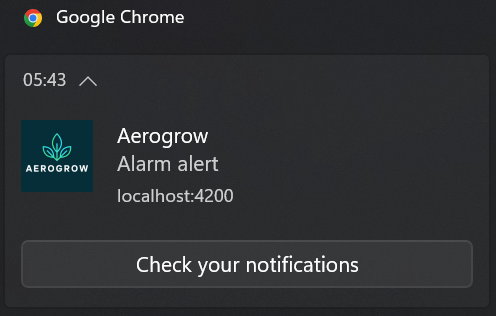
\includegraphics[width=.6\textwidth]{./Figures/Notificacion push.png}
	\caption{Ejemplo de notificacion \emph{push}.}
	\label{fig:notificacionPushEmail}
\end{figure}

En la figura \ref{fig:listaDeNotificaciones} se visualiza la pantalla del listado de notificaciones de un usuario. El listado se actualiza en tiempo real y se puede filtrar por período de tiempo y por cualquier campo de la tabla. Además, el usuario puede exportar los datos en formato xlsx y marcar las notificaciones como leídas.

\begin{figure}[H]
	\centering
	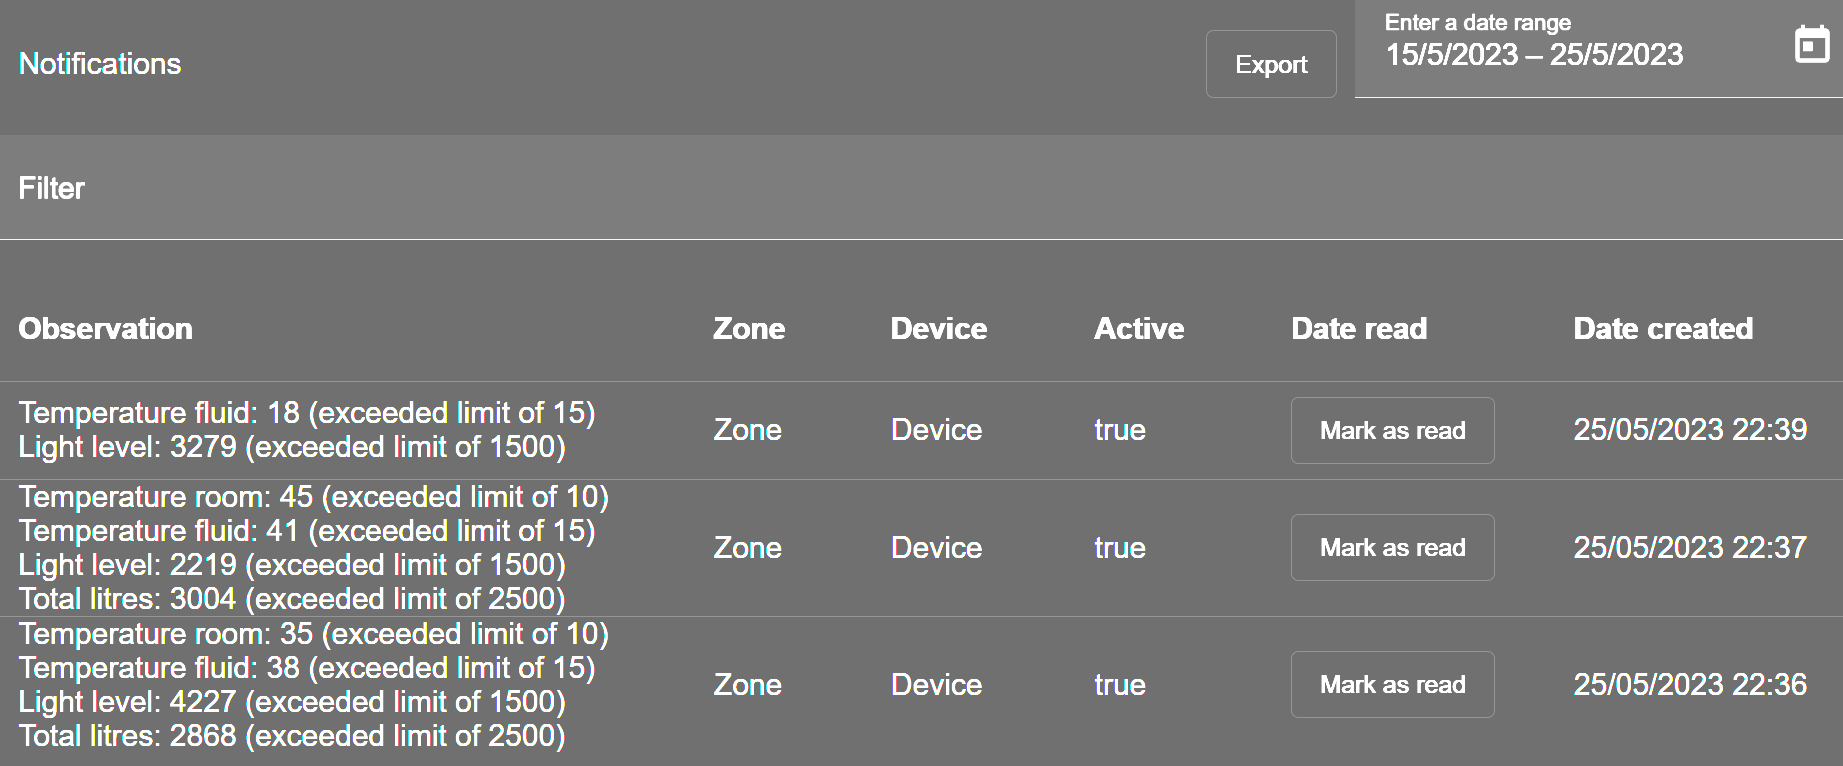
\includegraphics[width=.9\textwidth]{./Figures/Frontend lista de notificaciones.png}
	\caption{Pantalla de listado de notificaciones.}
	\label{fig:listaDeNotificaciones}
\end{figure}

En las figuras \ref{fig:tablaMedicionesDashboardDeZona}, \ref{fig:graficoMedicionesDashboardDeZona} y \ref{fig:cardsDashboardDeZona} se presentan los componentes que forman la pantalla de \emph{dashboard} de una zona. 

En la figura \ref{fig:tablaMedicionesDashboardDeZona} se visualiza el listado de mediciones de una zona. El listado se actualiza en tiempo real y se puede filtrar por período de tiempo y por cualquier campo de la tabla. Además, el usuario puede exportar los datos en formato xlsx.

\begin{figure}[H]
	\centering
	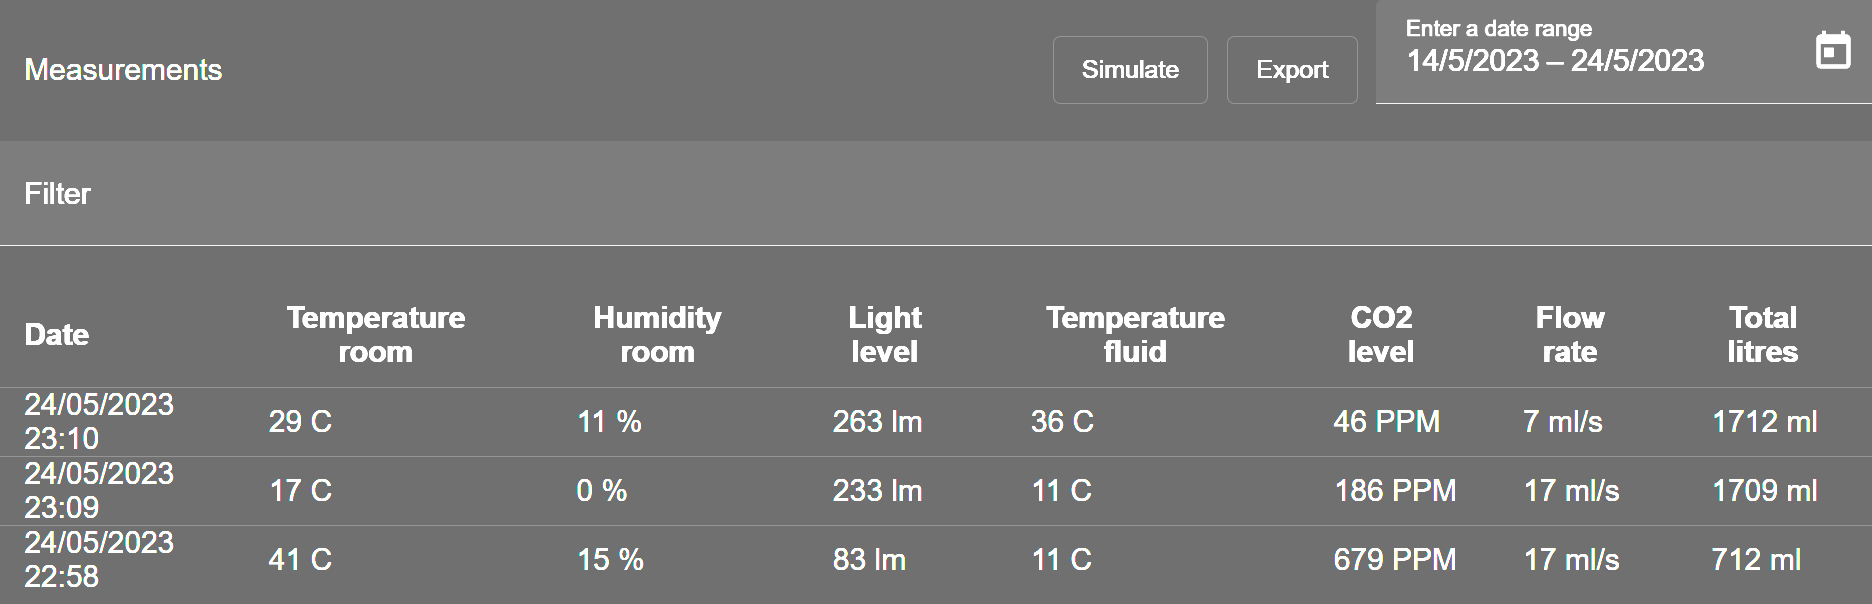
\includegraphics[width=.9\textwidth]{./Figures/Frontend dashboard de zona tabla.png}
	\caption{Listado de mediciones en vista de \textit{dashboard}.}
	\label{fig:tablaMedicionesDashboardDeZona}
\end{figure}

En la figura \ref{fig:graficoMedicionesDashboardDeZona} se visualiza el gráfico de las mediciones recibidas en el período de tiempo seleccionado. El componente permite seleccionar el tipo de atributo que se quiere graficar y se actualiza en tiempo real.

\begin{figure}[H]
	\centering
	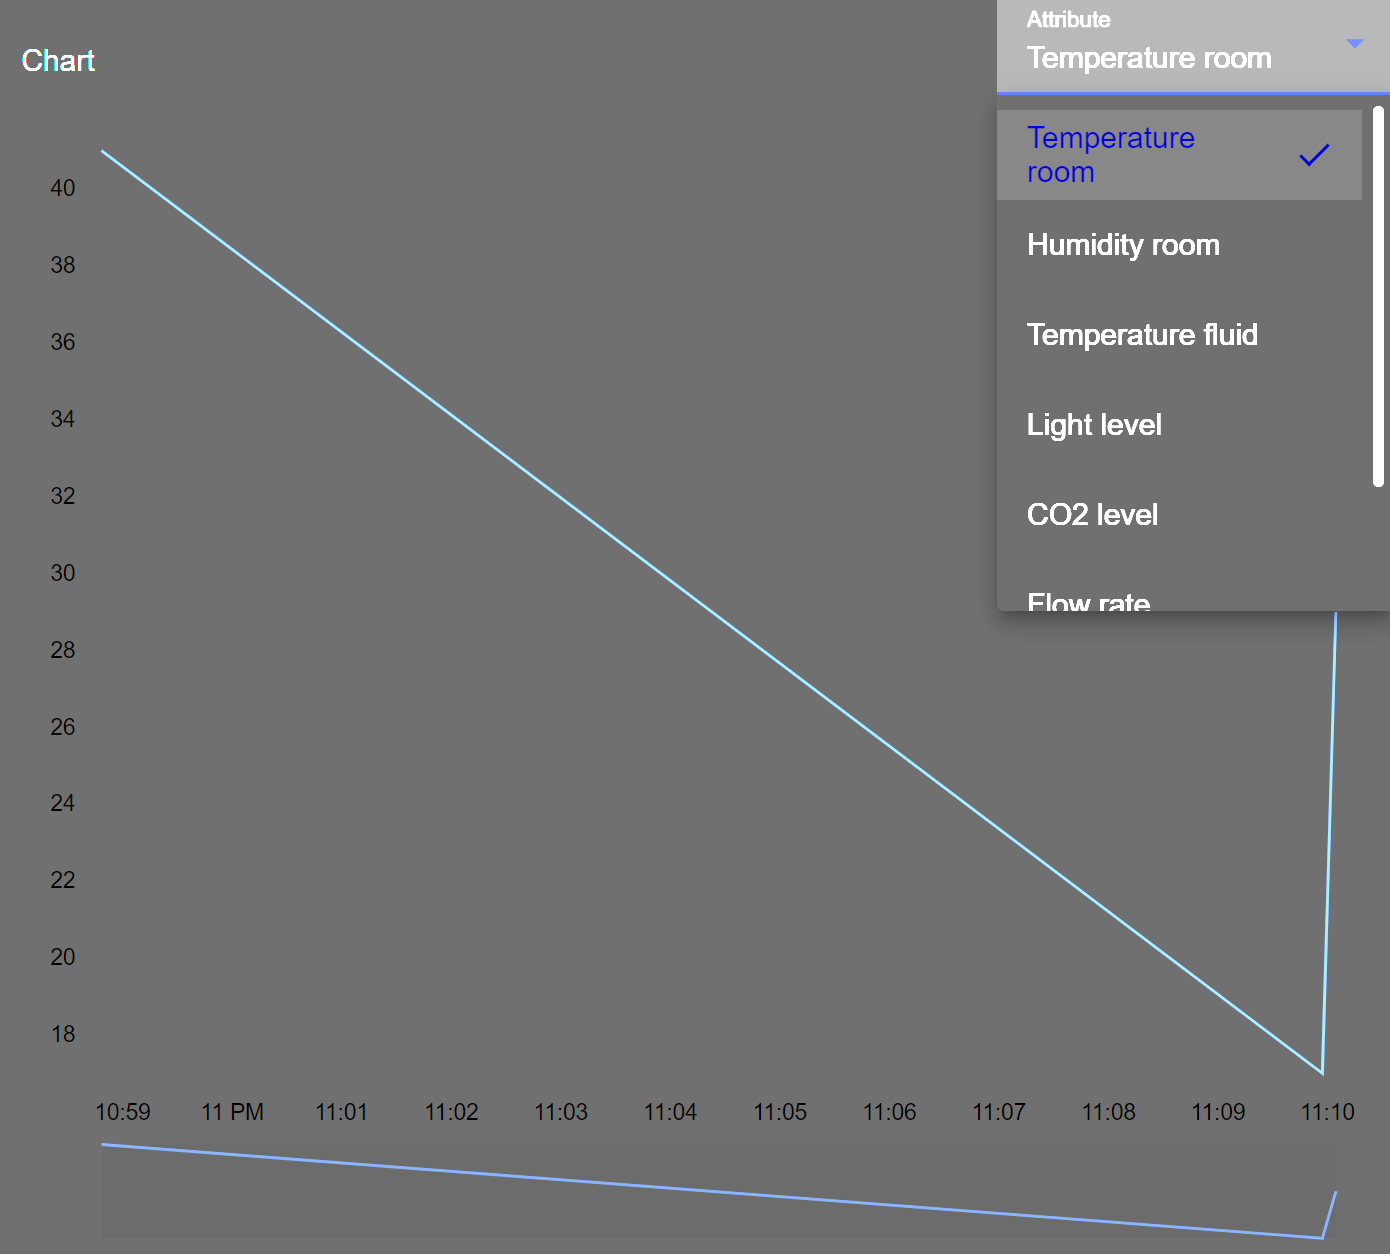
\includegraphics[width=.7\textwidth]{./Figures/Frontend dashboard de zona grafico.png}
	\caption{Gráfico de mediciones en vista de \textit{dashboard}.}
	\label{fig:graficoMedicionesDashboardDeZona}
\end{figure}

En la figura \ref{fig:cardsDashboardDeZona} se presentan las \emph{cards} del \emph{dashboard}. Las \textit{cards} se actualizan en tiempo real y permiten monitorear los datos de la última medición y accionar los \textit{relays} de la zona. 

\begin{figure}[H]
	\centering
	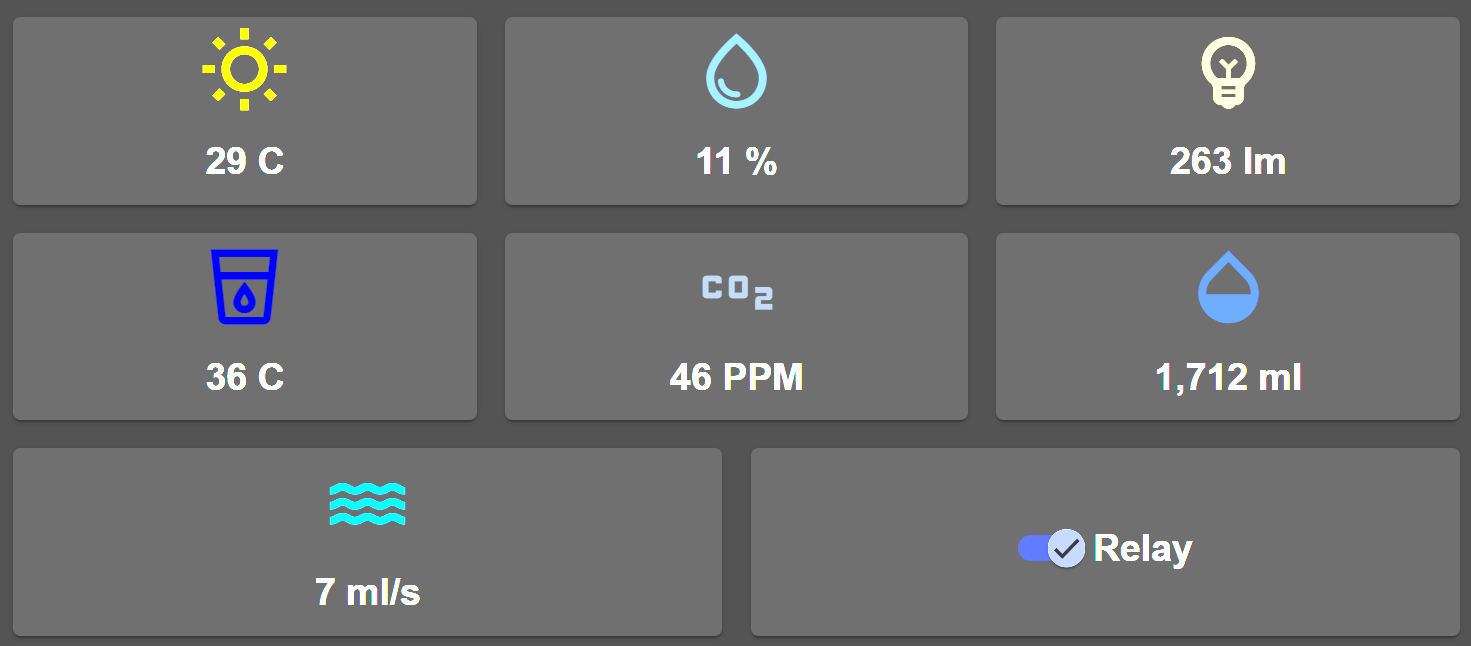
\includegraphics[width=.7\textwidth]{./Figures/Frontend dashboard de zona cards.png}
	\caption{\textit{Cards} en vista de \textit{dashboard}.}
	\label{fig:cardsDashboardDeZona}
\end{figure}

\section{Desarrollo del \emph{broker}}

El \emph{broker} fue desarrollado en Node.js mediante TypeScript y Aedes.

En el código \ref{cod:inicializacionBroker} se presenta la inicialización del \emph{broker} con certificados TLS. En las líneas 1 a 3 se obtienen los certificados. En las líneas 5 a 11 se configuran las opciones del \emph{broker}: se asignan los certificados, se solicita a los clientes que tengan certificados válidos  y se rechazan las conexiones que no tengan una autoridad de certificación \citep{WEBSITE:AUTORIDADDECERTIFICACION} válida. En la línea 12 se establece el número de puerto que utiliza el \emph{broker}. En las líneas 13 a 19 se crea el \emph{broker} con las opciones configuradas.

\begin{lstlisting}[label=cod:inicializacionBroker,caption=Inicialización del \emph{broker} con TLS.]
const ca = readFileSync("ssl/ca.crt");
const privateKey = readFileSync("./ssl/broker.key");
const certificate = readFileSync("./ssl/broker.crt");

const options: TlsOptions = {
   key: privateKey,
   cert: certificate,
   ca: ca,
   requestCert: true,
   rejectUnauthorized: true,
};
const mqttPort = 8883;
const mqttServer = createServer(options, aedes.handle);

mqttServer.listen(mqttPort, () => {
   console.log(
     `[server]: MQTT Server is running at mqtts://localhost:${mqttPort}`
   );
});
\end{lstlisting}

El \emph{broker} utiliza como medida extra de seguridad un proceso de autenticación mediante usuario y contraseña. En el código \ref{cod:autenticaciónBroker} se presenta el proceso de autenticación de los clientes. En las líneas 7 a 12 se verifica que el usuario y contraseña del cliente sea válido. En la línea 13 se autentica al cliente. En las líneas 16 a 19 se entrega  al cliente un error que indica que el usuario o la contraseña son inválidos.

\newpage
\begin{lstlisting}[label=cod:autenticaciónBroker,caption=Autenticación de clientes.]
aedes.authenticate = (
   _client: Client,
   username: Readonly<string | undefined>,
   password: Readonly<Buffer | undefined>,
   done: (error: AuthenticateError | null, success: boolean | null) => void
) => {
   if (
     username &&
     password &&
     username === mqttUsername &&
     Buffer.from(password).toString() === mqttPassword
   ) {
     return done(null, true);
   }

   const error = new Error() as AuthenticateError;
   error.returnCode = AuthErrorCode.BAD_USERNAME_OR_PASSWORD;

   return done(error, false);
};
\end{lstlisting}

En el código \ref{cod:procesoPublishBroker} se presenta el proceso de validación de mensajes publicados en los tópicos. En las líneas 8 a 11 se verifica que el tópico del mensaje sea válido. En las líneas 12 a 13 se le entrega al cliente un error que indica que no está autorizado para publicar el mensaje. En las líneas 18 a 21 se obtiene el \emph{payload} del mensaje para crear una nueva medición. En las líneas 23 a 28 se le entrega al cliente un error si la medición no pudo ser creada. En la línea 32 se indica que el mensaje publicado es válido.

\newpage
\begin{lstlisting}[label=cod:procesoPublishBroker,caption=Validación de mensajes.]
aedes.authorizePublish = async (
   client: Client | null,
   packet: PublishPacket,
   done: (error?: AuthenticateError | null | undefined) => void
) => {
   const error = new Error() as AuthenticateError;

   if (
     packet.topic != topicMeasurements &&
     !packet.topic.includes(topicRelays)
   ) {
     error.returnCode = AuthErrorCode.NOT_AUTHORIZED;
     return done(error);
   }

   if (packet.topic == topicMeasurements) {
     try {
       const measurementPayload: MeasurementPayload = JSON.parse(
         packet.payload.toString()
       );
       await createMeasurement(measurementPayload, socket);
     } catch (errorPayload) {
       console.error(
         "[server]: Publish measurement payload has failed",
         error
       );
       error.returnCode = AuthErrorCode.SERVER_UNAVAILABLE;
       return done(error);
     }
   }

    return done(null);
};
\end{lstlisting}

\section{Desarrollo sobre el microcontrolador}

El \emph{software} del microcontrolador fue desarrollado mediante la plataforma Espressif 32 \citep{WEBSITE:ESPRESSIF32} y el \emph{framework} Arduino \citep{WEBSITE:ARDUINO}. La elección del \emph{framework} es debida a los siguientes factores: 

\begin{itemize}
	\item Facilidad de uso.
	\item Amplia comunidad y soporte.
	\item Compatibilidad con una gran cantidad de placas y microcontroladores.
	\item Desarrollo rápido.
\end{itemize}

%Los datos del sistema son obtenidos de los sensores por el microcontrolador cada un segundo, sin embargo para determinar el caudal diario de la zona de cultivo se crea un acumulador que suma la cantidad de agua por segundo y cuando termina el día es reiniciado.

En el código \ref{cod:conexionWiFi} se presentan los procesos de conexión al Wi-Fi y configuración de los certificados TLS. En las líneas 1, 2 y 3 se importan las bibliotecas necesarias y las variables de entorno. En las líneas 5 a 7 se crean las variables para el cliente de la biblioteca y el nombre y contraseña de la red. En la línea 15 se inicia la conexión con las credenciales de la red. En las líneas 22 a 25 se monta el sistema de archivos del microcontrolador. En las líneas 27, 28 y 29 se aplican los certificados TLS al cliente Wi-Fi.

\newpage
\begin{lstlisting}[label=cod:conexionWiFi,caption=Conexión Wi-Fi y configuración de los certificados TLS]
#include "WiFiClientSecure.h"
#include "SPIFFS.h"
#include "secrets.h"

WiFiClientSecure wifiClient;
const char* ssid = SSID;
const char* password = PASSWORD;

void setupWifi() {
  delay(10);
  Serial.println();
  Serial.print("Connecting to ");
  Serial.println(ssid);

  WiFi.begin(ssid, password);

  while (WiFi.status() != WL_CONNECTED) {
    delay(500);
    Serial.print(".");
  }

  if(!SPIFFS.begin(true)){
    Serial.println("An Error has occurred while mounting SPIFFS");
    return;
  }
  
  wifiClient.setCACert(getFileAsString("/ca.crt"));
  wifiClient.setCertificate(getFileAsString("/esp.crt"));
  wifiClient.setPrivateKey(getFileAsString("/esp.key"));
  
  Serial.println("");
  Serial.println("WiFi connected");
  Serial.println("IP address: ");
  Serial.println(WiFi.localIP());
}
\end{lstlisting}

En el código \ref{cod:conexionMQTT} se presenta el proceso de conexión al \emph{broker} MQTT. En las líneas 1, 2 y 3 se importan las bibliotecas necesarias y las variables de entorno.  En las  líneas 5 y 6 se crean las variables para utilizar las dependencias importadas. En las líneas 8 a 11 se crea un tipo de estructura para agrupar a los \textit{relays}. En las líneas 13 a 17 se crean las variables para la dirección, credenciales y tópicos del \emph{broker}. En las líneas 18 a 20 se crea una variable utilizando la estructura de \textit{relays}. En la línea 23 se establece la dirección y el puerto del \emph{broker}. En la línea 24 se establece el método de \emph{callback}. En las líneas 28 a 44 se intenta realizar la conexión mientras no esté activa. En las líneas 48 a 51 se ejecuta el método para conectarse al \emph{broker} si la conexión no está activa.

\newpage
\begin{lstlisting}[label=cod:conexionMQTT,caption=Conexión al \emph{broker} MQTT]
#include "WiFiClientSecure.h"
#include <PubSubClient.h>
#include "secrets.h"

WiFiClientSecure wifiClient;
PubSubClient mqttClient(wifiClient);

typedef struct {
  int pin;
  char* id;
} Relay;

const char* mqttServer = BROKER_IP;
const char* clientUsername = BROKER_USERNAME;
const char* clientPassword = BROKER_PASSWORD;
const char* deviceId = DEVICE_ID;
const char* topicRelays = "relays/";
Relay relays[NUM_RELAYS] = {
  { 16, RELAY_ID }
};

void setupMQTT(){
  mqttClient.setServer(mqttServer, 8883);
  mqttClient.setCallback(callback);
}

void reconnect() {
  while (!mqttClient.connected()) {
    Serial.print("Attempting MQTT connection...");
    if (mqttClient.connect(deviceId, clientUsername, clientPassword)) {
      Serial.println("connected");
      for(int i = 1; i <= NUM_RELAYS; i++){
        char buffer[64];
        strcpy(buffer, topicRelays);
        strcat(buffer, relays[i-1].id);
        mqttClient.subscribe(buffer);
      }
    } else {
      Serial.print("failed, rc=");
      Serial.print(mqttClient.state());
      Serial.println(" try again in 5 seconds");
      delay(5000);
    }
  }
}

void loop() {
  if (!mqttClient.connected()) {
    reconnect();
  }
  mqttClient.loop();
  ...
}
\end{lstlisting}
% Chapter Template

\chapter{Ensayos y resultados} % Main chapter title

\label{Chapter4} % Change X to a consecutive number; for referencing this chapter elsewhere, use \ref{ChapterX}

En este capítulo se detallan las pruebas unitarias realizadas al \textit{frontend} y \textit{backend} y la prueba de integración del sistema completo.

%----------------------------------------------------------------------------------------
%	SECTION 1
%----------------------------------------------------------------------------------------

\section{Pruebas del \emph{frontend}}

Para probar el \textit{frontend} se decidió utilizar una batería de pruebas unitarias \citep{WEBSITE:UNITTESTING} creadas con Jasmine y Karma. Estás fueron completamente automatizadas para garantizar y asegurar la calidad de código. Se realizaron 208 pruebas unitarias para lograr un 100\% de cobertura de código.

En la figura \ref{fig:unitTestingFrontend} se visualiza el proceso de ejecución de las pruebas unitarias con Karma.

\begin{figure}[H]
	\centering
	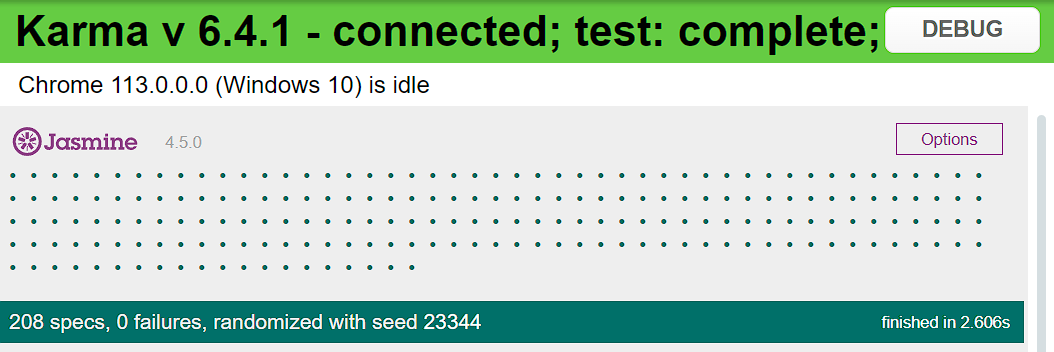
\includegraphics[width=.9\textwidth]{./Figures/Frontend unit testing.png}
	\caption{Pruebas unitarias.}
	\label{fig:unitTestingFrontend}
\end{figure}

En la figura \ref{fig:codeCoverageFrontend} se visualiza la cobertura de código del \emph{frontend}.

\begin{figure}[H]
	\centering
	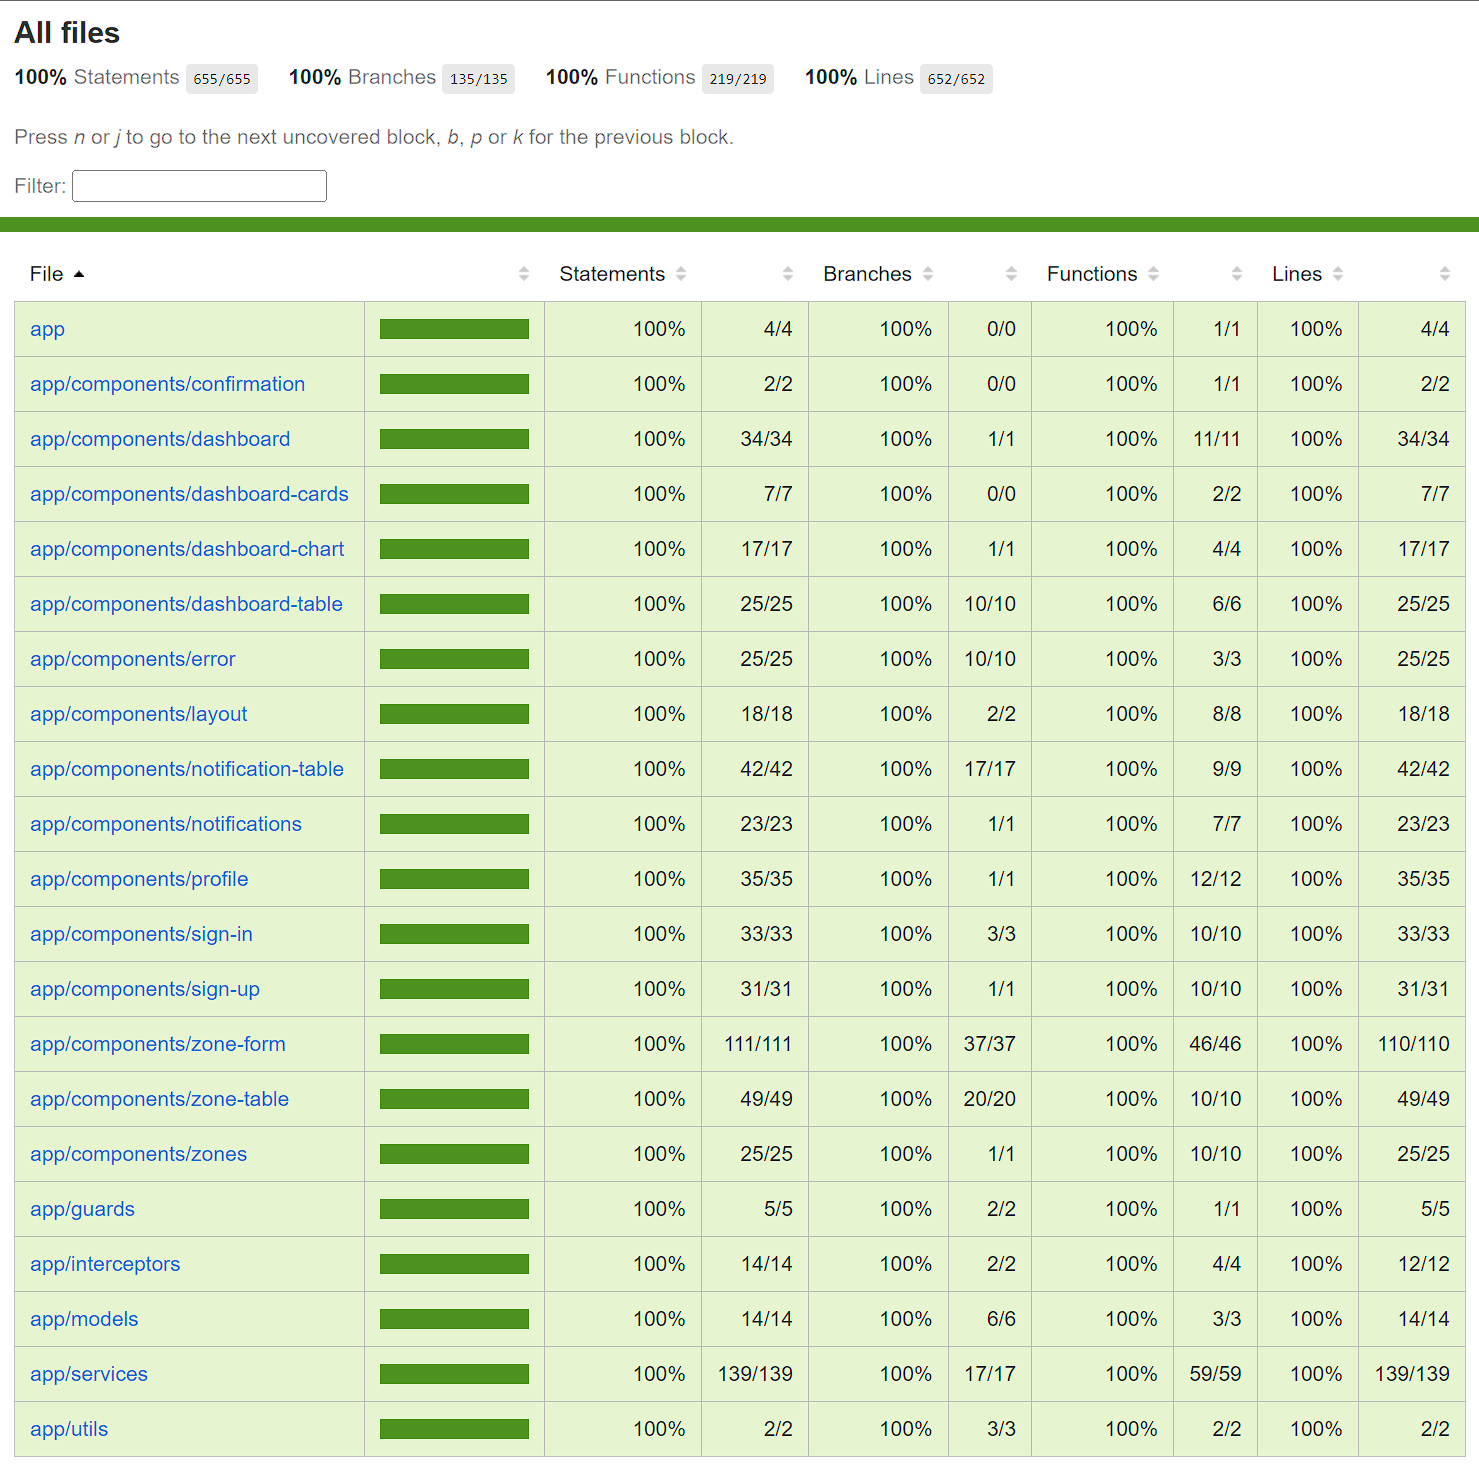
\includegraphics[width=.9\textwidth]{./Figures/Frontend code coverage.png}
	\caption{Cobertura de código.}
	\label{fig:codeCoverageFrontend}
\end{figure}

A modo de ejemplo se presenta en el código \ref{cod:unitTestFrontend} la prueba unitaria del \emph{guard} utilizado para la autenticación de rutas. En la línea 2  se crea un \emph{mock} del \textit{Router} de Angular. En las líneas 4 a 6 se reinicia el método del \emph{mock} creado. En las líneas 8 a 19 se crea el contexto de prueba. En las líneas 21 y 29 se crean los dos casos de prueba. En las líneas 22 a 25 se crea un \emph{mock} del servicio de autenticación para simular que el usuario tiene una sesión activa. En la línea 26 se verifica que el método del \emph{mock} del \textit{Router} fue ejecutado. En las líneas 30 a 33 se crea un \emph{mock} del servicio de autenticación del \emph{frontend} para simular que el usuario no tiene una sesión activa. En la línea 34 se verifica que el método del \emph{mock} del \textit{Router} no fue ejecutado.

\begin{lstlisting}[label=cod:unitTestFrontend,caption=Prueba unitaria del \emph{guard} de autenticación de rutas.]
describe('authGuard', () => {
  const mockRouter = jasmine.createSpyObj<Router>(['navigate']);

  afterEach(() => {
    mockRouter.navigate.calls.reset();
  });

  const setup = (authService: unknown) => {
    TestBed.configureTestingModule({
      providers: [
        { provide: AuthService, useValue: authService },
        { provide: Router, useValue: mockRouter },
      ],
    });

    return TestBed.runInInjectionContext(() =>
      authGuard({} as ActivatedRouteSnapshot, {} as RouterStateSnapshot)
    );
  };

  it('should allow to continue', () => {
    const mockAuthService: unknown = {
      isLoggedIn: () => true,
    };
    setup(mockAuthService);
    expect(mockRouter.navigate).not.toHaveBeenCalled();
  });

  it('should redirect to /sign-in path', () => {
    const mockAuthService: unknown = {
      isLoggedIn: () => false,
    };
    setup(mockAuthService);
    expect(mockRouter.navigate).toHaveBeenCalled();
  });
});
\end{lstlisting}

En la figura \ref{fig:certificadosTLSDelFrontendAplicados} se presenta el resultado de configurar los certificados TLS.

\begin{figure}[H]
	\centering
	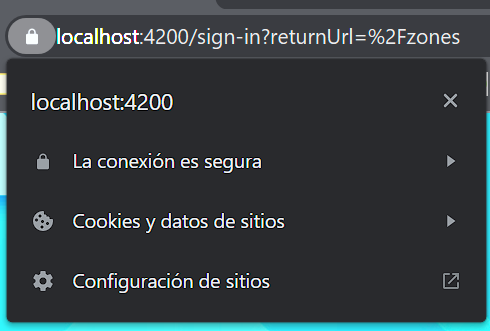
\includegraphics[width=.5\textwidth]{./Figures/Frontend certificados TLS.png}
	\caption{Certificados TLS aplicados.}
	\label{fig:certificadosTLSDelFrontendAplicados}
\end{figure} 

Se utilizó Lighthouse para realizar una auditoría del \emph{frontend}, los aspectos evaluados son: rendimiento, accesibilidad, mejores prácticas, SEO y un chequeo del tipo de aplicación: si es PWA se evalúa su implementación, caso contrario se restan puntos al resultado de la auditoría. La herramienta fue aplicada a las tres pantallas más demandantes del sistema: \emph{dashboard} de una zona, listado de zonas y listado de notificaciones.

En la figura \ref{fig:lighthouseDashboardZona} se presenta el resultado de la auditoría realizada sobre la pantalla de \emph{dashboard} de una zona.

\begin{figure}[H]
	\centering
	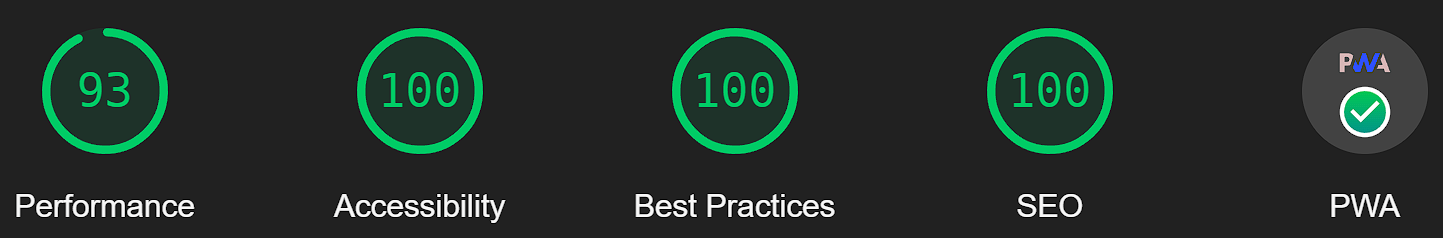
\includegraphics[width=.9\textwidth]{./Figures/Lighthouse dashboard.png}
	\caption{Auditoría realizada sobre la pantalla de \emph{dashboard} de una zona}
	\label{fig:lighthouseDashboardZona}
\end{figure}

En la figura \ref{fig:lighthouseListadoZonas} se presenta el resultado de la auditoría realizada sobre la pantalla de listado de zonas.

\begin{figure}[H]
	\centering
	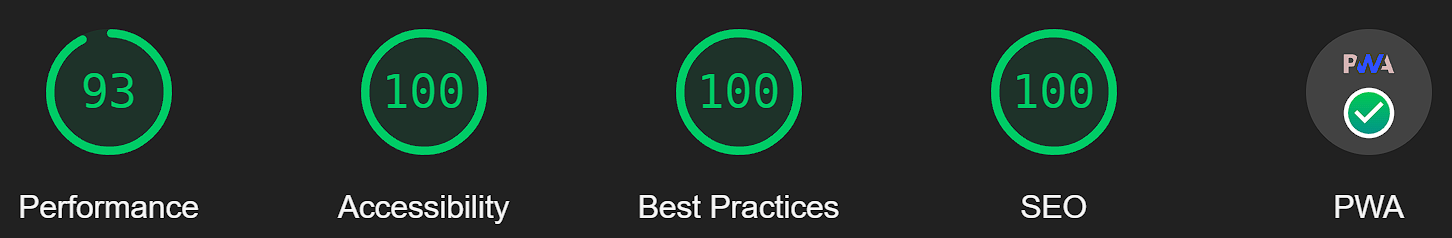
\includegraphics[width=.9\textwidth]{./Figures/Lighthouse zonas.png}
	\caption{Auditoría realizada sobre la pantalla de listado de zonas}
	\label{fig:lighthouseListadoZonas}
\end{figure}

En la figura \ref{fig:lighthouseListadoZonas} se presenta el resultado de la auditoría realizada sobre la pantalla de listado de notificaciones.

\begin{figure}[H]
	\centering
	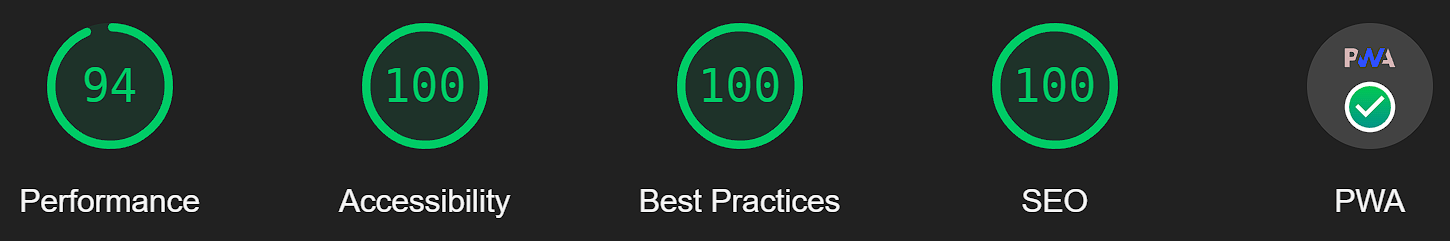
\includegraphics[width=.9\textwidth]{./Figures/Lighthouse notificaciones.png}
	\caption{Auditoría realizada sobre la pantalla de listado de notificaciones}
	\label{fig:lighthouseListadoZonas}
\end{figure}

Las tres auditorías realizadas obtuvieron la puntuación máxima en todas las categorías, excepto en rendimiento. Para alcanzar la máxima puntuación en rendimiento, es necesario reducir o eliminar el código JavaScript que no se utiliza en la aplicación.
 
\section{Pruebas del \emph{backend}}

Para probar el \textit{backend} se decidió utilizar una batería de pruebas unitarias creadas con Jest. Estás fueron completamente automatizadas para garantizar y asegurar la calidad de código. Se realizaron 78 pruebas unitarias para lograr un 100\% de cobertura de código. 

En la figuras \ref{fig:unitTestingBackend1} y \ref{fig:unitTestingBackend2} se visualiza el proceso de ejecución de las pruebas unitarias con Jest.

\begin{figure}[H]
	\centering
	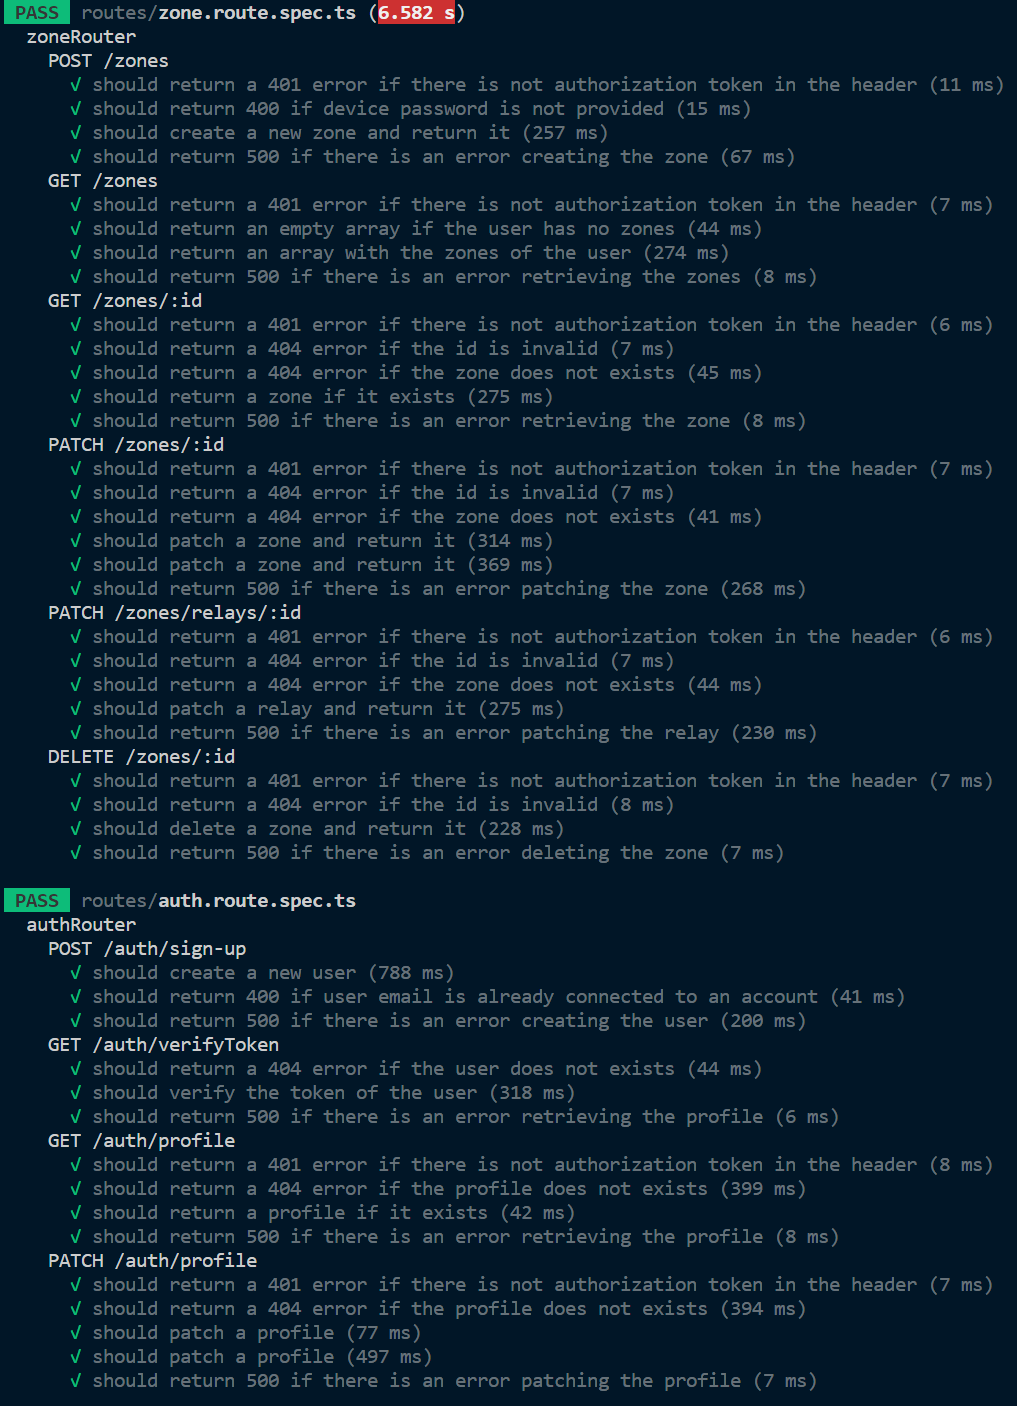
\includegraphics[width=.9\textwidth]{./Figures/Backend unit testing.png}
	\caption{Pruebas unitarias parte 1 de 2.}
	\label{fig:unitTestingBackend1}
\end{figure}

\begin{figure}[H]
	\centering
	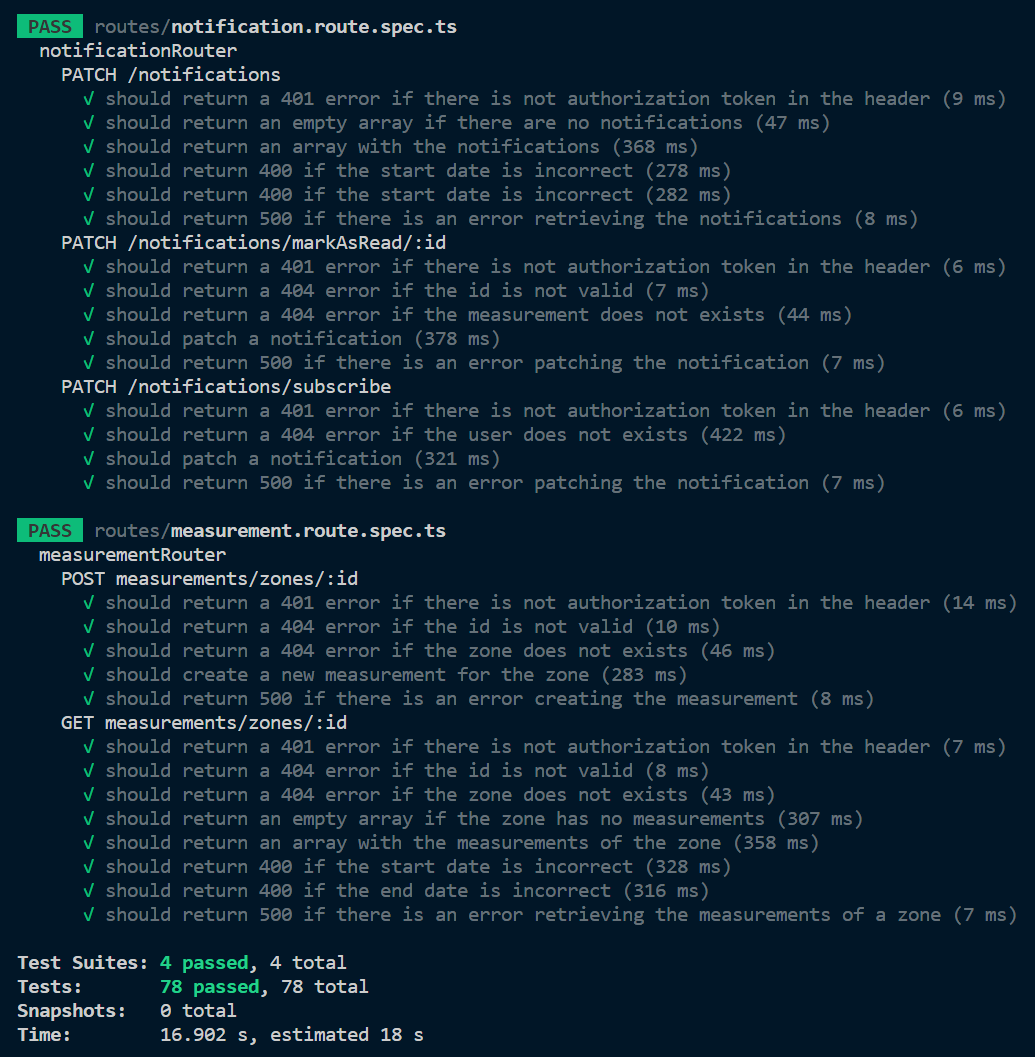
\includegraphics[width=.9\textwidth]{./Figures/Backend unit testing 2.png}
	\caption{Pruebas unitarias parte 2 de 2.}
	\label{fig:unitTestingBackend2}
\end{figure}


En la figura \ref{fig:codeCoverageBackend} se visualiza la cobertura de código del \emph{backend}.

\begin{figure}[H]
	\centering
	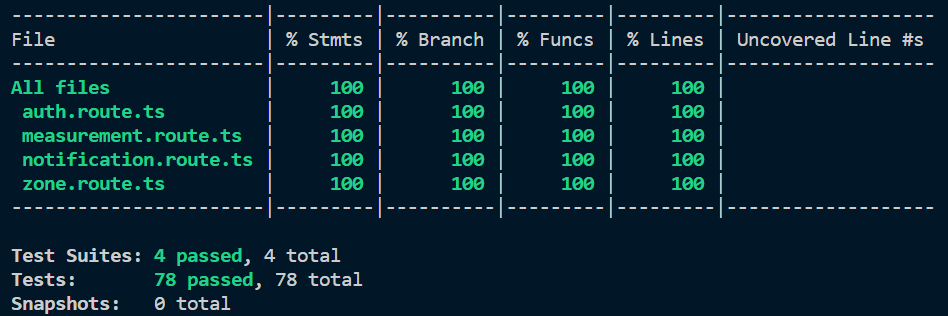
\includegraphics[width=.9\textwidth]{./Figures/Backend code coverage.png}
	\caption{Cobertura de código.}
	\label{fig:codeCoverageBackend}
\end{figure}

A modo de ejemplo, se presenta en el código \ref{cod:unitTestBackend} la prueba unitaria del \emph{endpoint} \textit{/zones}. En las líneas 2, 9, 19 y 31 se crean los casos de prueba. En las línea 3 a 6 se simula una \emph{request} al \emph{endpoint} sin haber configurado el \textit{authorization header}, además se valida que el código de la respuesta sea 401. En las líneas 10 a 16 se simula una \emph{request} al \emph{endpoint}, además se valida que el código de la respuesta sea 200 y que el \textit{body} sea una lista vacía. En la línea 20 se crea una zona. En las líneas 21 a 25 se simula una \emph{request} al \emph{endpoint} y se valida que el código de respuesta sea 200. En la línea 27 se elimina la zona creada. En la línea 28 se valida que el \textit{body} de la respuesta sea una lista con la zona creada. En las líneas  32 a 34 se crea un \emph{mock} sobre un método del ORM Mongoose para simular un error cuando se ejecute. En las líneas 36 a 40 se simula una \emph{request} al \emph{endpoint} y se valida que el código de respuesta sea 500.

\begin{lstlisting}[label=cod:unitTestBackend,caption=Prueba unitaria del \emph{endpoint /zones}]
describe("GET /zones", () => {
  it("should return a 401 error if there is not authorization token in the header", async () => {
    const response = await request(app)
      .get("/api/zones")
      .trustLocalhost()
      .expect(401);
  });

  it("should return an empty array if the user has no zones", async () => {
    const response = await request(app)
      .get("/api/zones")
      .trustLocalhost()
      .set("Authorization", `Bearer ${token}`)
      .expect(200);

    expect(response.body).toEqual([]);
   });

  it("should return an array with the zones of the user", async () => {
    await createZone();
    const response = await request(app)
      .get("/api/zones")
      .trustLocalhost()
      .set("Authorization", `Bearer ${token}`)
      .expect(200);

    await deleteZone();
    expect(response.body).toEqual([zone]);
  });

  it("should return 500 if there is an error retrieving the zones", async () => {
    jest.spyOn(Zone, "find").mockImplementation(() => {
      throw new Error();
    });

    const response = await request(app)
      .get("/api/zones")
      .trustLocalhost()
      .set("Authorization", `Bearer ${token}`)
      .expect(500);

    jest.spyOn(Zone, "find").mockRestore();
    expect(response.statusCode).toEqual(500);
  });
});
\end{lstlisting} 

%\section{Pruebas del \emph{broker}}

%Con el objetivo de validar la conexión con certificados TLS al \emph{broker} MQTT se realizaron cuatro pruebas manuales:

%\begin{itemize}
	%\item Caso de prueba uno: intento de conexión sin credenciales ni certificados.
	%\item Caso de prueba uno: intento de conexión con credenciales pero sin certificados.
	%\item Caso de prueba tres: intento de conexión con credenciales y certificados inválidos.
	%\item Caso de prueba cuatro: intento de conexión con credenciales y certificados válidos.
%\end{itemize}

\section{Prueba final de integración}

Se realizó una prueba final de integración para verificar el correcto funcionamiento del sistema.

En la figura \ref{fig:diagramaBancoDePruebas} se visualiza un diagrama del banco de pruebas con los componentes y relaciones que lo forman.

\begin{figure}[H]
	\centering
	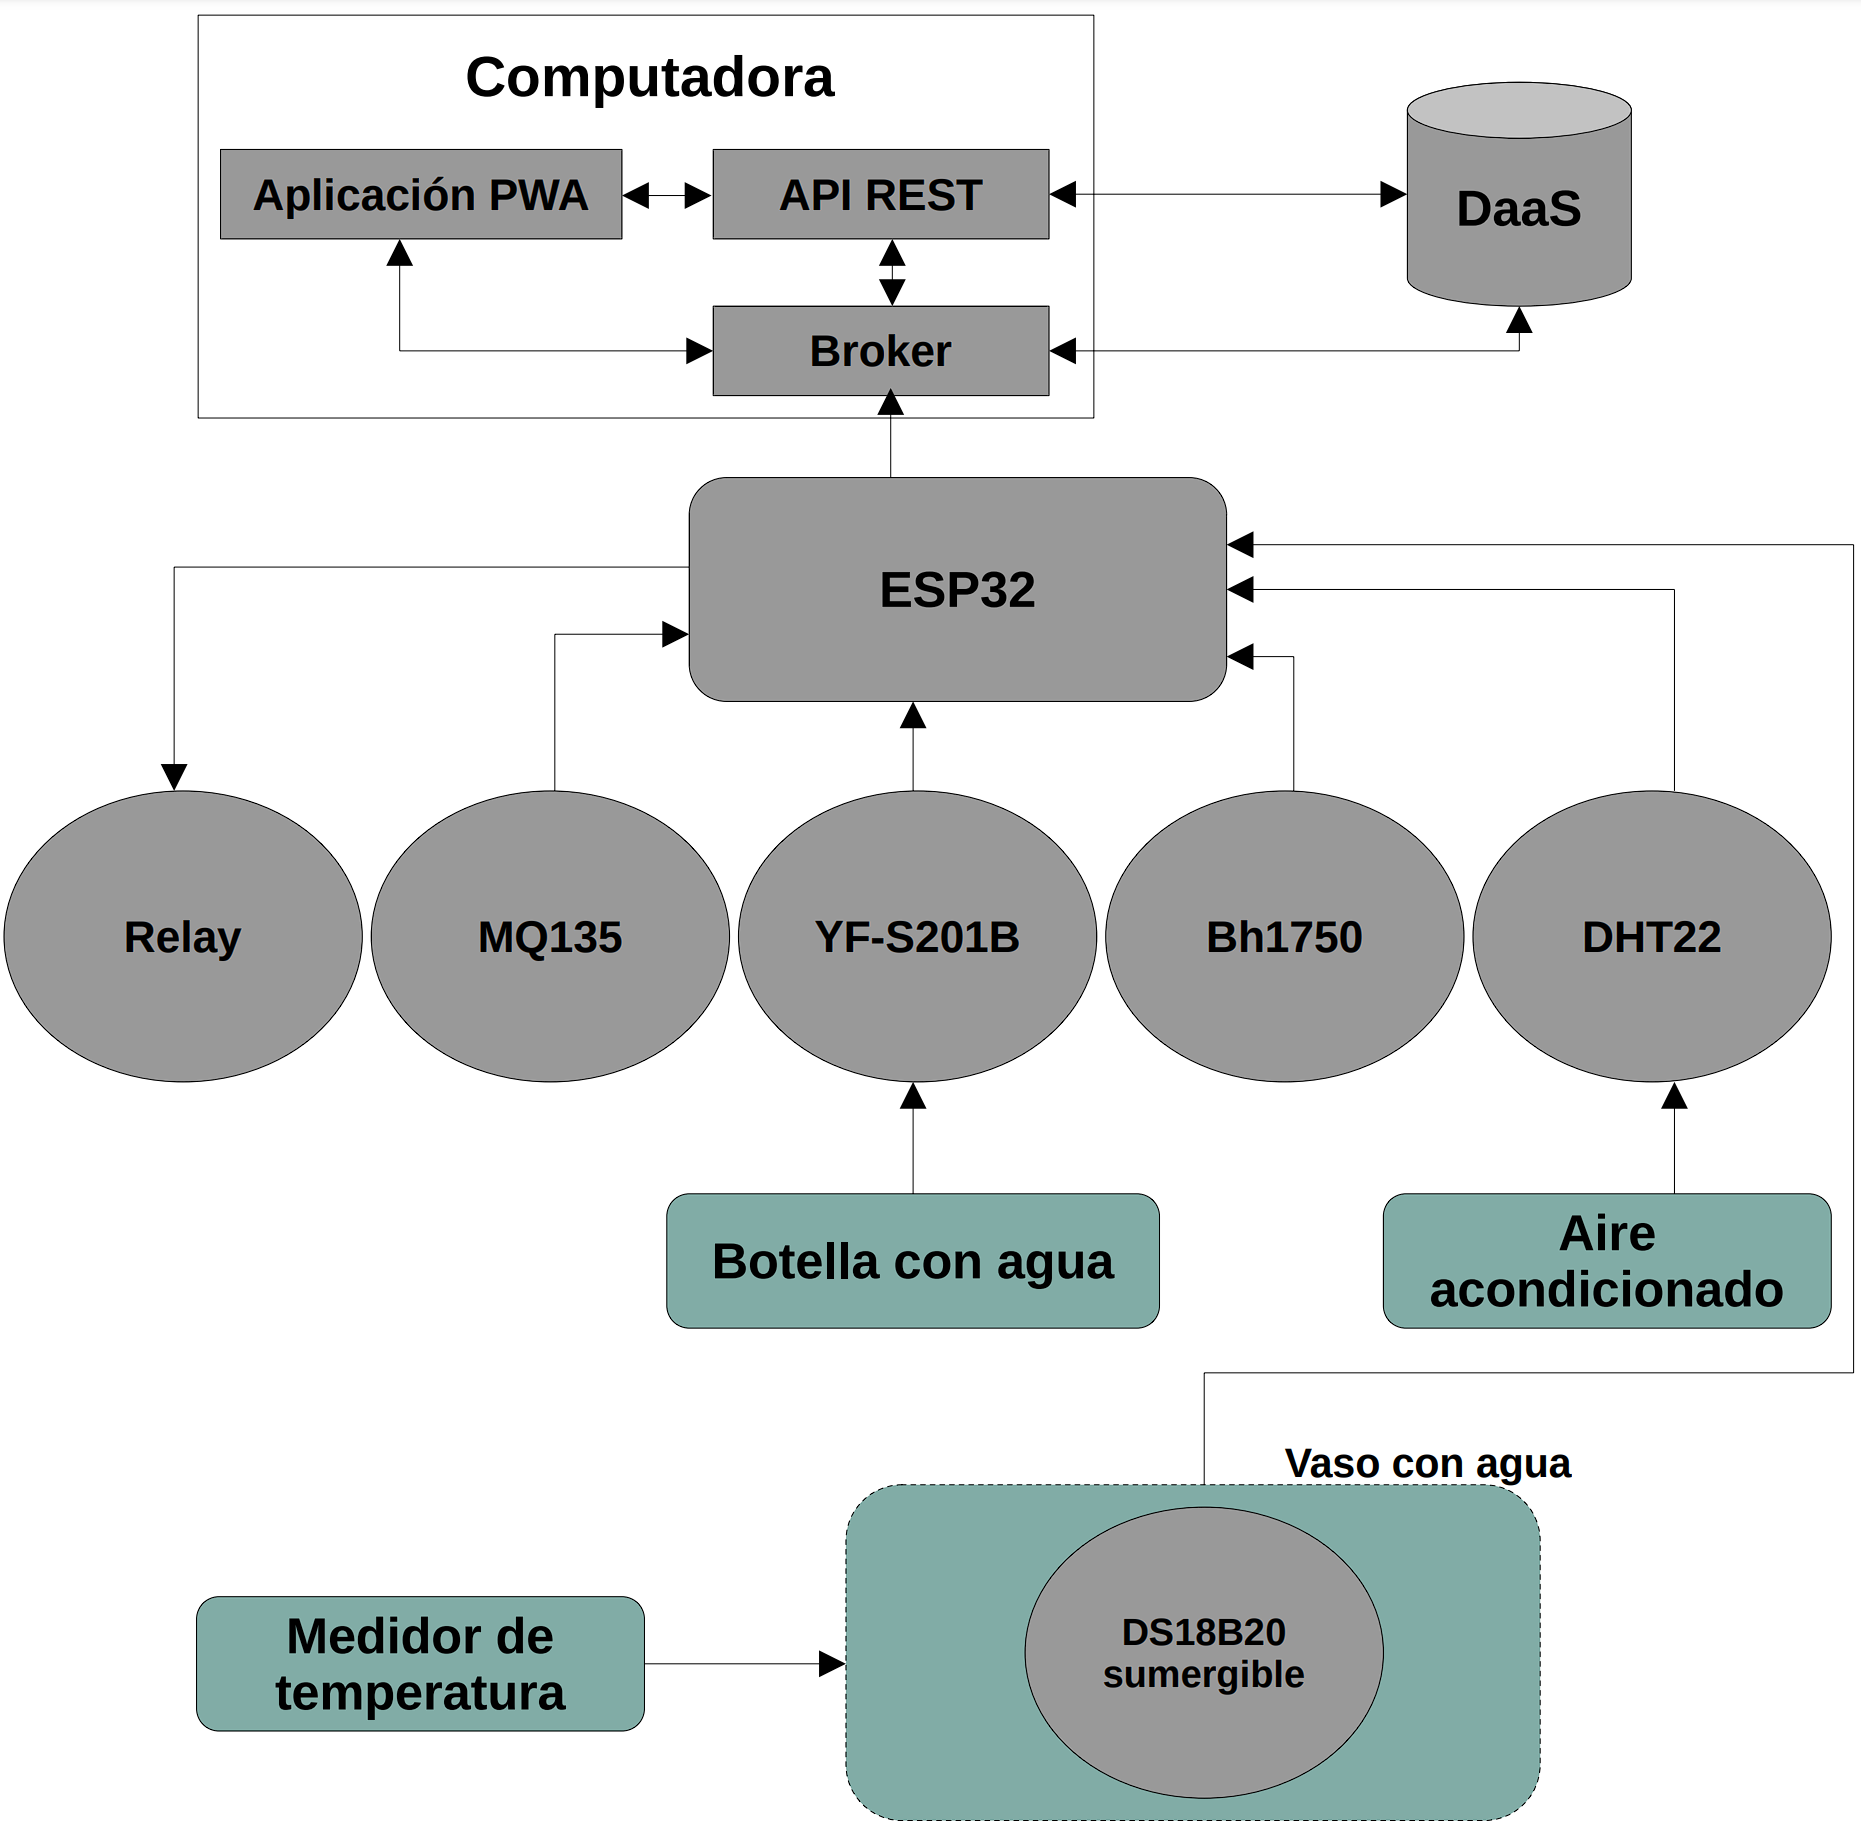
\includegraphics[width=.9\textwidth]{./Figures/Diagrama del banco de pruebas v2.png}
	\caption{Diagrama del banco de pruebas.}
	\label{fig:diagramaBancoDePruebas}
\end{figure}

Los pasos previos de configuración de la prueba consistieron en:

\begin{itemize}
	\item Inicializar el \textit{backend} y el \textit{broker} por medio del comando npm run dev. En la figura \ref{fig:inicializacionBackendIntegracion} se visualiza el resultado de la ejecución del comando.

\begin{figure}[H]
	\centering
	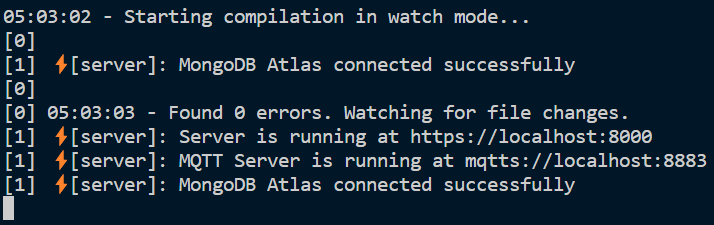
\includegraphics[width=.9\textwidth]{./Figures/Backend inicializacion.png}
	\caption{Inicialización del \emph{backend}.}
	\label{fig:inicializacionBackendIntegracion}
\end{figure}

	\item Inicializar el \textit{frontend} por medio del comando npm run lite-server. En la figura \ref{fig:inicializacionFrontendIntegracion} se visualiza el resultado de la ejecución del comando.

\begin{figure}[H]
	\centering
	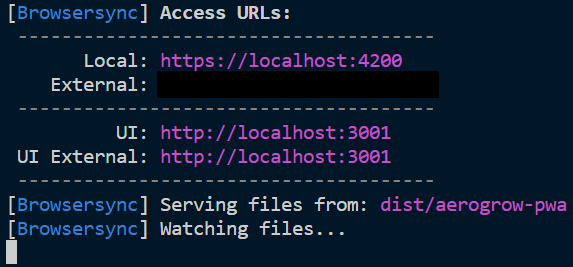
\includegraphics[width=.9\textwidth]{./Figures/Frontend inicializacion.png}
	\caption{Inicialización del \emph{frontend}.}
	\label{fig:inicializacionFrontendIntegracion}
\end{figure}

	\item Iniciar sesión en el sistema con una cuenta creada previamente.
	\item Crear una nueva zona de cultivo que tenga un \textit{relay} y dos alarmas. La primera alarma se dispara si la temperatura del ambiente es diferente a 1 °C y tiene una acción asociada que activa el \textit{relay} si la alarma se dispara por una temperatura mayor a 1 °C. La segunda alarma se dispara si la temperatura del líquido es menor a 1 °C o mayor a 2 °C. En las figuras \ref{fig:crearNuevaZonaIntegracion} y \ref{fig:listadoDeZonasIntegracion} se visualiza el proceso de creación de la zona.
	
	\begin{figure}[H]
	\centering
	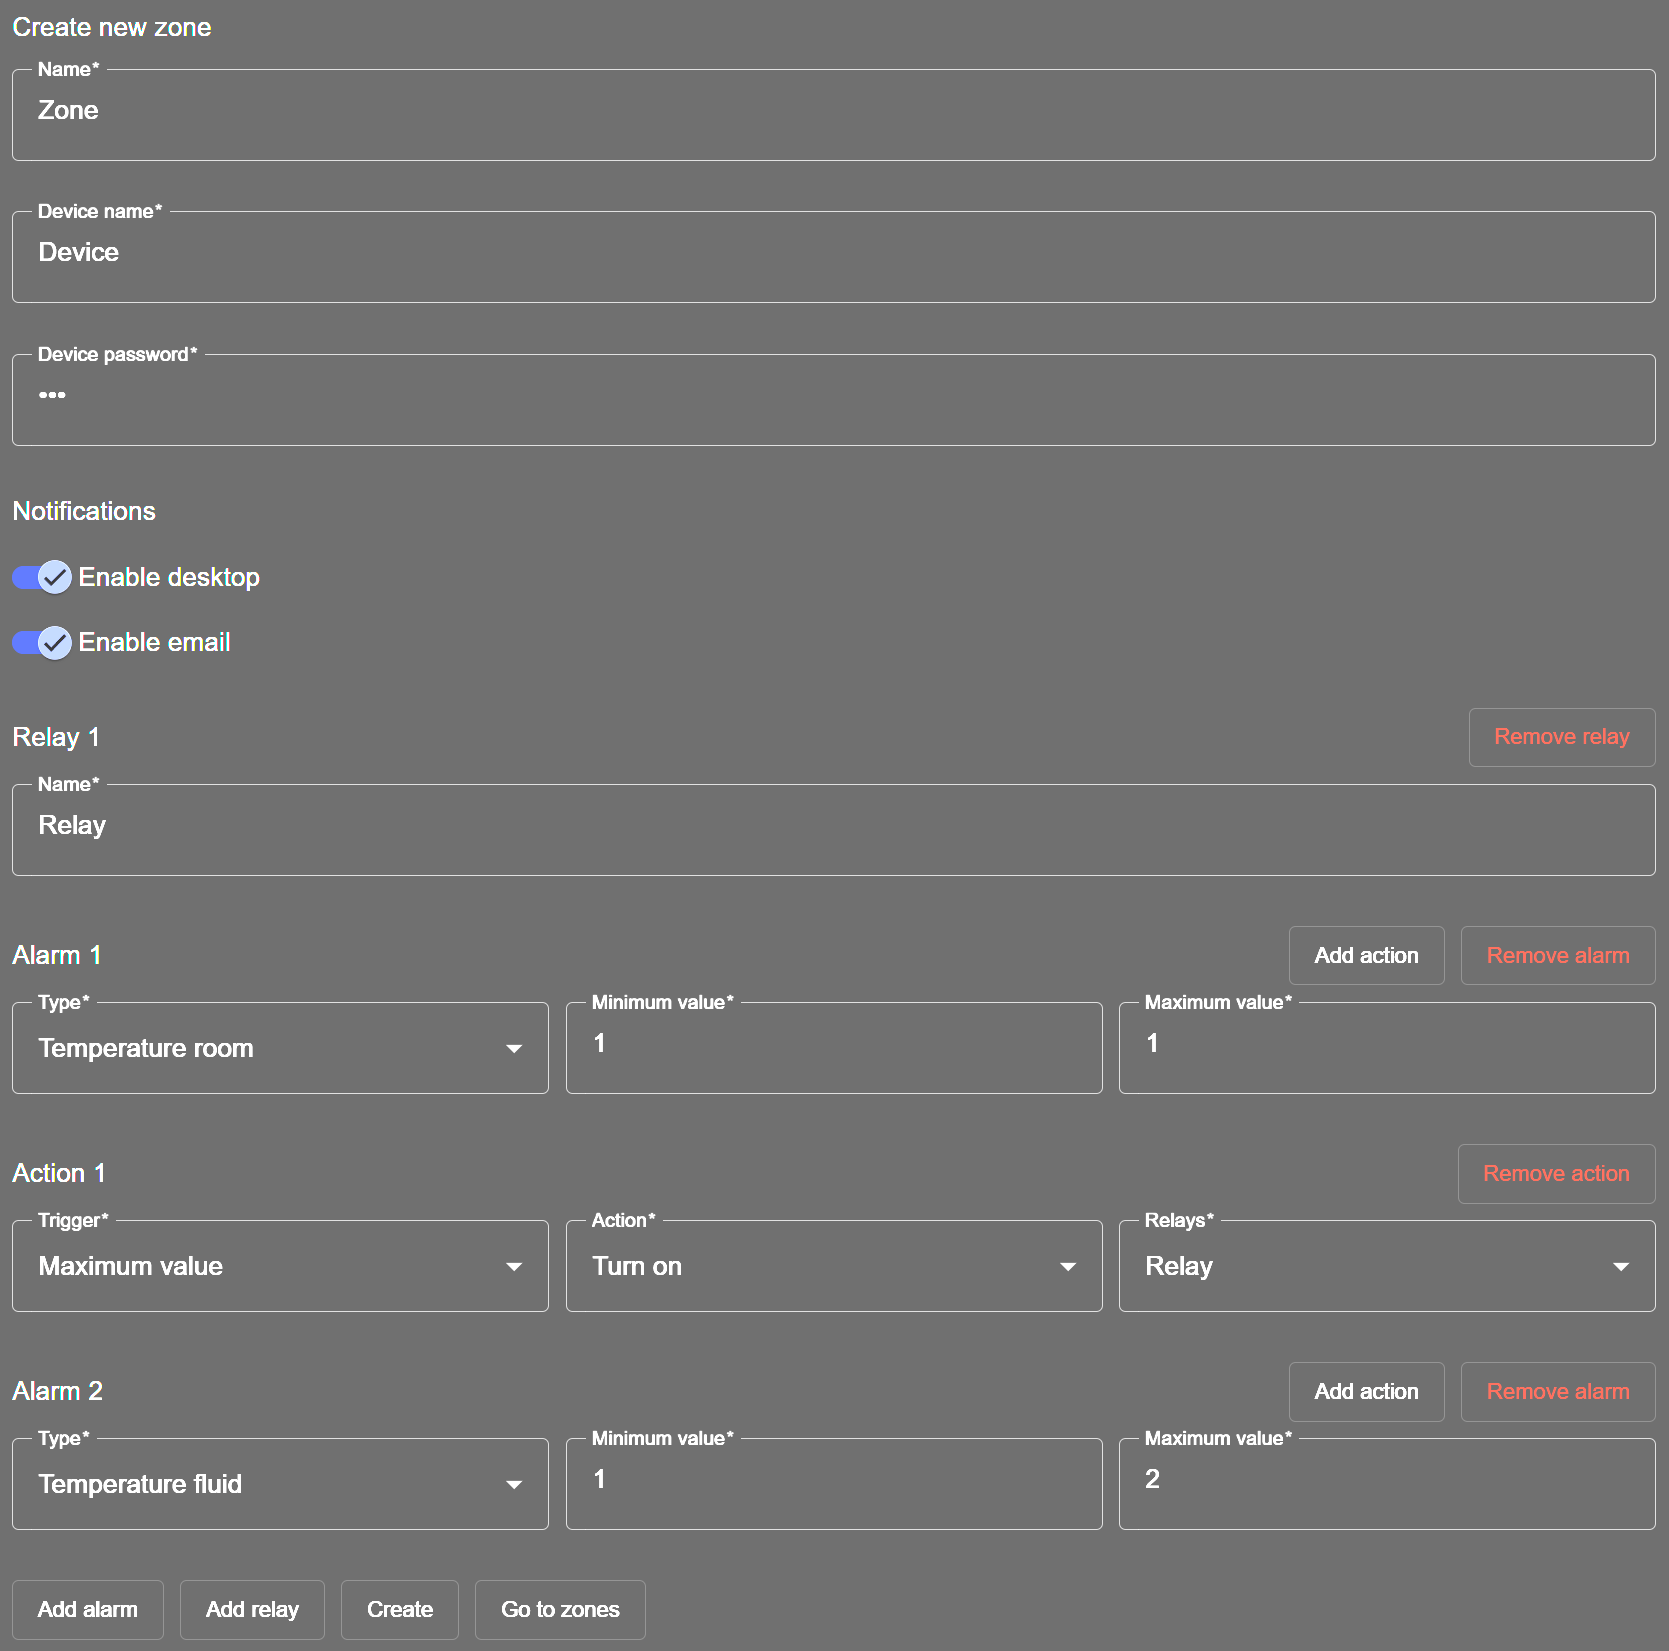
\includegraphics[width=.9\textwidth]{./Figures/Frontend crear nueva zona.png}
	\caption{Pantalla de creación de una zona.}
	\label{fig:crearNuevaZonaIntegracion}
\end{figure}

\begin{figure}[H]
	\centering
	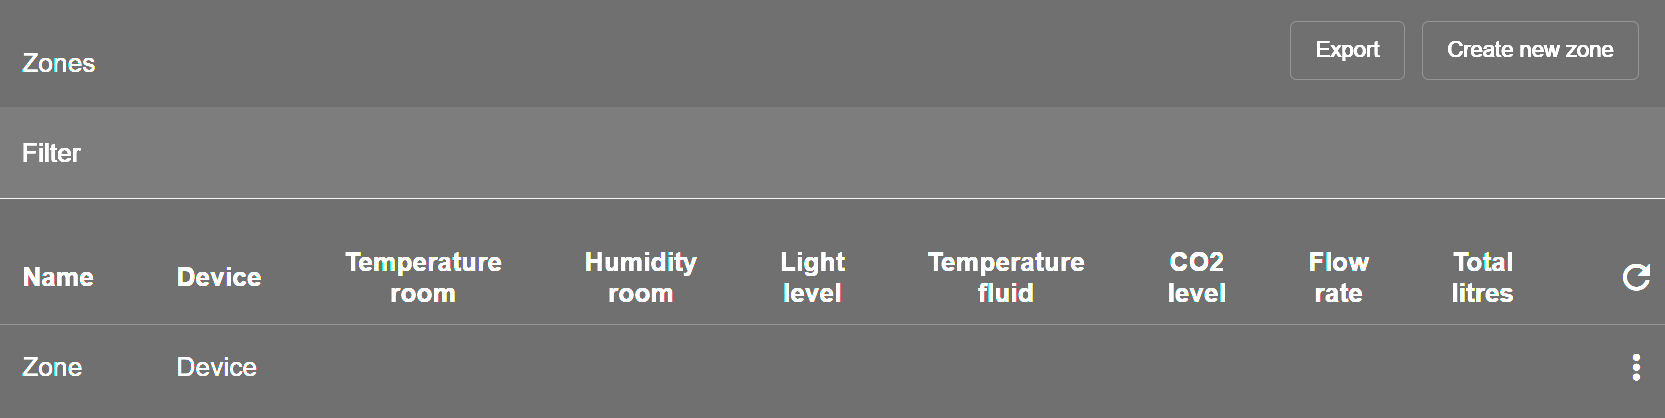
\includegraphics[width=.9\textwidth]{./Figures/Frontend nueva zona creada.png}
	\caption{Pantalla de listado de zonas.}
	\label{fig:listadoDeZonasIntegracion}
\end{figure}
	
	\item Conectar y configurar el \textit{software} del microcontrolador con las credenciales de la zona. En la figura \ref{fig:configuracionMicrocontroladorConfiguradoCredenciales} se presenta la configuración de credenciales en el microcontrolador.
	
\begin{figure}[H]
	\centering
	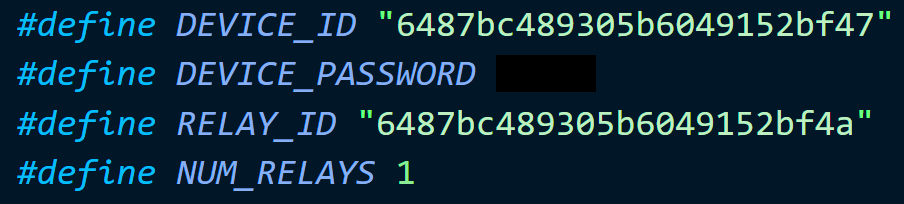
\includegraphics[width=.9\textwidth]{./Figures/Microcontrolador configuracion credenciales.png}
	\caption{Configuración de credenciales en el microcontrolador.}
	\label{fig:configuracionMicrocontroladorConfiguradoCredenciales}
\end{figure}

	\item Programar el microcontrolador con las nuevas credenciales.

	\item Monitorear el microcontrolador. En la figura \ref{fig:microcontroladorMonitoreo} se observa una parte del proceso de monitoreo mediante la extensión PlatformIO.
	
\begin{figure}[H]
	\centering
	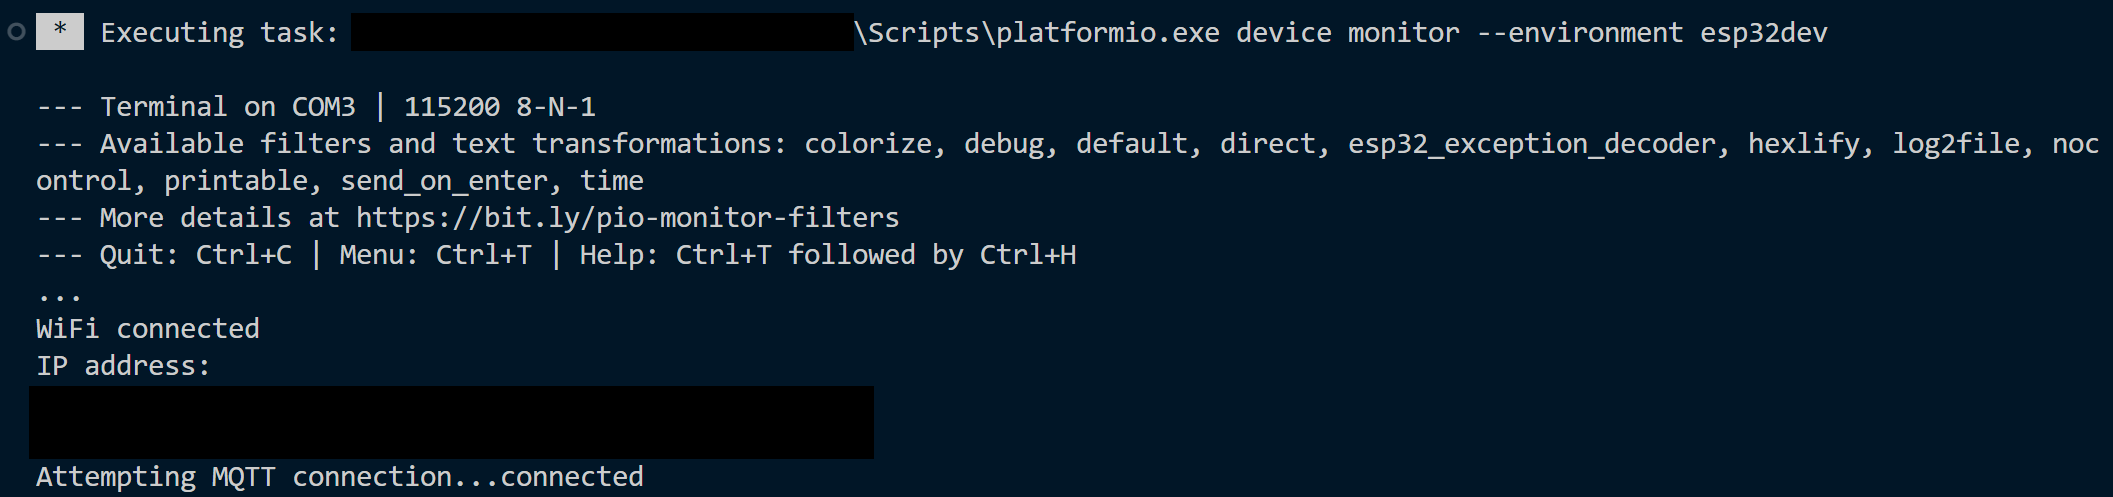
\includegraphics[width=.9\textwidth]{./Figures/Microcontrolador monitoreo.png}
	\caption{Monitoreo del microcontrolador.}
	\label{fig:microcontroladorMonitoreo}
\end{figure}
\end{itemize}

Para asegurar que se active la primera alarma, se colocó el sensor DHT22 en un ambiente con un aire acondicionado \citep{WEBSITE:BGHR410A} encendido en una temperatura de 24 °C por 30 minutos. 

Para asegurar que se dispare la segunda alarma, se colocó el sensor DS18B20 en un recipiente con agua previamente validada con un medidor externo \citep{WEBSITE:TP101} para asegurar que su temperatura sea de al menos 20 °C. 

Para que todos los sensores reporten valores al microcontrolador, se ingresó agua manualmente al sensor YF-S201B.

En las figuras \ref{fig:frontendListadoMedicionesPruebaDeIntegracion} y \ref{fig:frontendDashboardDeZonaPruebaDeIntegracion} se observa la pantalla de \textit{dashboard} de la zona con la medición registrada y el \textit{relay} activo. 

\begin{figure}[H]
	\centering
	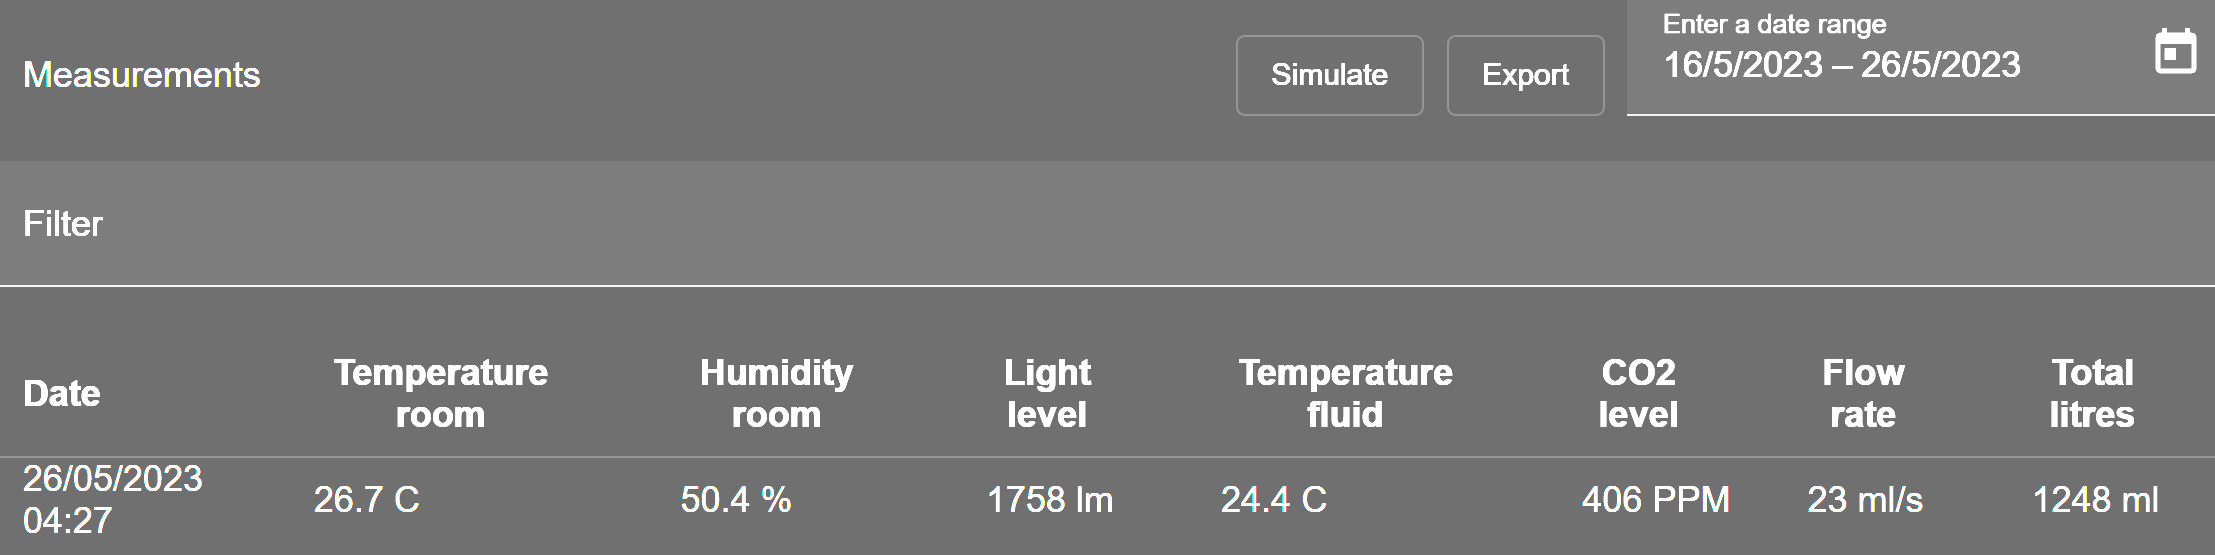
\includegraphics[width=.9\textwidth]{./Figures/Frontend listado de mediciones prueba de integracion.png}
	\caption{Listado de mediciones en vista de \textit{dashboard}.}
	\label{fig:frontendListadoMedicionesPruebaDeIntegracion}
\end{figure}

\begin{figure}[H]
	\centering
	\includegraphics[width=.9\textwidth]{./Figures/Frontend dashboard de zona cards prueba de integracion.png}
	\caption{\textit{Cards} en vista de \textit{dashboard}.}
	\label{fig:frontendDashboardDeZonaPruebaDeIntegracion}
\end{figure}

En las figuras \ref{fig:frontendListadoDeNotificacionesPruebaDeIntegracion}, \ref{fig:notificacionEmailPruebaDeIntegracion} y \ref{fig:notificacionDesktopruebaDeIntegracion} se presentan las notificaciones enviadas por el sistema al activarse la alarma.

\begin{figure}[H]
	\centering
	\includegraphics[width=.9\textwidth]{./Figures/Frontend listado de notificaciones prueba de integracion.png}
	\caption{Pantalla de listado de notificaciones.}
	\label{fig:frontendListadoDeNotificacionesPruebaDeIntegracion}
\end{figure}

\begin{figure}[H]
	\centering
	\includegraphics[width=.8\textwidth]{./Figures/Notificacion email prueba de integracion.png}
	\caption{\textit{Email} enviado por el sistema.}
	\label{fig:notificacionEmailPruebaDeIntegracion}
\end{figure}

\begin{figure}[H]
	\centering
	\includegraphics[width=.5\textwidth]{./Figures/Notificacion desktop prueba de integracion.png}
	\caption{Notificación \textit{push} enviada por el sistema.}
	\label{fig:notificacionDesktopruebaDeIntegracion}
\end{figure}

\section{Comparación con el estado del arte}

En la tabla \ref{tab:comparativaTrabajoSolucionesNacionalesInternacionales} se presenta la comparación de las características y funcionalidades entre los sistemas comerciales encontrados en el mercado nacional e internacional y el trabajo realizado llamado Aerogrow.

\begin{table}[H]
	\centering
	\caption[Comparativa entre soluciones comerciales similares y el trabajo realizado]{Comparativa entre soluciones comerciales similares y el trabajo realizado.}
	\begin{tabular}{l c c c}    
		\toprule
		\textbf{Funcionalidad} & \textbf{Smartcultiva} & \textbf{My Autogrow} & \textbf{Aerogrow}\\
		\midrule
		MQTT & Sí & Sí & Sí \\
		Sistema de alertas & Sí & Sí & Sí\\
		Acciones automatizadas & Sí & No & Sí\\
		Notificaciones \emph{push} & No & No & Sí\\
		Notificaciones \textit{email} & Sí & Sí & Sí\\
		\shortstack{Accionamiento de \\ dispositivos externos} & Sí & No & Sí\\
		Escalabilidad en sensores & Limitado & Limitado & Alta\\
		Tipo de aplicación & Móvil y web & Web & PWA\\
		\bottomrule
		\hline
	\end{tabular}
	\label{tab:comparativaTrabajoSolucionesNacionalesInternacionales}
\end{table}

En la tabla \ref{tab:comparativaTrabajoSolucionesPublicacionesCientificas} se presenta la comparación de las características y funcionalidades entre los sistemas encontrados en publicaciones científicas y el trabajo realizado.

\begin{table}[H]
	\centering
	\caption[Comparativa entre soluciones similares encontradas en publicaciones científicas y el trabajo realizado]{Comparativa entre soluciones similares encontradas en publicaciones científicas y el trabajo realizado.}
	\begin{tabular}{l c c c}    
		\toprule 
		\textbf{Funcionalidad} & \textbf{\textit{Monitoring Soil (...)}} & \textbf{\textit{A Smart (...)}}  & \textbf{Aerogrow}\\
		\midrule
		MQTT & Sí & No  & Sí\\
		LoRa & Sí & Sí  & No\\
		Sistema de alertas & No & Sí & Sí\\
		\shortstack{Acciones \\ automatizadas} & No & No & Sí\\
		Notificaciones \emph{push} & No & No & Sí\\
		Notificaciones \textit{email} & No & Sí & Sí\\
		\shortstack{Accionamiento de \\ dispositivos externos} & No & No & Sí\\
		\shortstack{Escalabilidad en \\ sensores} & Media & Media & Alta\\
		Tipo de aplicación & Web & Web & PWA\\
		\bottomrule
		\hline
	\end{tabular}
	\label{tab:comparativaTrabajoSolucionesPublicacionesCientificas}
\end{table}

De acuerdo a la comparación realizada, el trabajo elaborado se destaca por permitir recibir notificaciones \emph{push} y por la escalabilidad para añadir nuevos sensores. Sin embargo, se debe tener en cuenta los siguientes factores:

\begin{itemize}
\item Smartcultiva y este trabajo son las únicas soluciones que permiten crear acciones automatizadas cuando se activa una alerta. 
\item Smartcultiva y este trabajo son las únicas soluciones que permiten el accionamiento de dispositivos externos.
\item Las dos publicaciones científicas soportan el uso del protocolo LoRa.
\end{itemize} 
% Chapter Template

\chapter{Conclusiones} % Main chapter title

\label{Chapter5} % Change X to a consecutive number; for referencing this chapter elsewhere, use \ref{ChapterX}

En este capítulo se muestran las conclusiones sobre el trabajo realizado y se presentan algunas mejoras como posible trabajo futuro.

%----------------------------------------------------------------------------------------

%----------------------------------------------------------------------------------------
%	SECTION 1
%----------------------------------------------------------------------------------------

\section{Resultados obtenidos}

En este trabajo se completó el diseño, desarrollo y \textit{testing} de un sistema de gestión de cultivos aeropónicos.

Para evaluar los resultados obtenidos del trabajo es importante destacar los siguientes factores:
\begin{itemize}
	\item Se cumplió con la planificación en tiempo y forma aunque no se siguió exactamente con el orden de desarrollo planteado para cada tarea.
	\item No se manifestó ninguno de los riesgos previamente identificados en la planificación.
	\item Luego de realizar un análisis de los requerimientos, se concluye que todos fueron cumplidos. Sin embargo, como se menciona en la sección \ref{sec:observaciones} se realizaron dos modificaciones en el trabajo que afectaron algunos requerimientos: se decidió reemplazar la aplicación SSR por una PWA y se realizaron modificaciones en los datos a almacenar en el DaaS.
\end{itemize}

Fueron de gran utilidad los conocimientos adquiridos a lo largo de la especialización. A continuación, se enumeran las asignaturas que tuvieron mayor relevancia:
\begin{itemize}
	\item Gestión de proyectos.
	\item Arquitectura de protocolos.
	\item Gestión de grandes volúmenes de datos.
	\item Desarrollo de aplicaciones multiplataforma.
	\item Ciberseguridad en Internet de las Cosas.
\end{itemize}

%\section{Conclusiones generales }

%La idea de esta sección es resaltar cuáles son los principales aportes del trabajo realizado y cómo se podría continuar. Debe ser especialmente breve y concisa. Es buena idea usar un listado para enumerar los logros obtenidos.

%Algunas preguntas que pueden servir para completar este capítulo:

%\begin{itemize}
%\item ¿Cuál es el grado de cumplimiento de los requerimientos?
%\item ¿Cuán fielmente se puedo seguir la planificación original (cronograma incluido)?
%\item ¿Se manifestó algunos de los riesgos identificados en la planificación? ¿Fue efectivo el plan de mitigación? ¿Se debió %aplicar alguna otra acción no contemplada previamente?
%\item Si se debieron hacer modificaciones a lo planificado ¿Cuáles fueron las causas y los efectos?
%\item ¿Qué técnicas resultaron útiles para el desarrollo del proyecto y cuáles no tanto?
%\end{itemize}


%----------------------------------------------------------------------------------------
%	SECTION 2
%----------------------------------------------------------------------------------------

\section{Trabajo futuro}

A continuación se detallan las principales líneas de acción para dar continuidad a este trabajo:

\begin{itemize}
\item Mejorar el \emph{responsive} de las tablas del \emph{frontend}.
\item Incorporar SSR a la PWA.
\item Incorporar sensor de pH de la solución nutritiva.
\item Incorporar sensor de TDS de la solución nutritiva.
\item Incorporar estadísticas y más gráficos para el \emph{dashboard} de las zonas de cultivo.
\item Permitir crear más de un dispositivo por zona de cultivo.
\item Permitir seleccionar qué sensores se quiere asociar a cada dispositivo de las zonas de cultivo.
\item Desarrollar pruebas unitarias para el \emph{broker}.
\item Añadir multidioma al sistema utilizando i18n \citep{WEBSITE:ANGULARI18N}.
\item Permitir al usuario seleccionar las unidades a utilizar en las mediciones, por ejemplo: utilizar Fahrenheit o Celsius para las temperaturas.
\item Calibrar los sensores del sistema.
\item Realizar pruebas de campo en un entorno real.
\item Integrar el sistema en un gabinete.
\item Desplegar el sistema a un entorno \emph{cloud}.
\end{itemize} 

%----------------------------------------------------------------------------------------
%	CONTENIDO DE LA MEMORIA  - APÉNDICES
%----------------------------------------------------------------------------------------

\appendix % indicativo para indicarle a LaTeX los siguientes "capítulos" son apéndices

% Incluir los apéndices de la memoria como archivos separadas desde la carpeta Appendices
% Descomentar las líneas a medida que se escriben los apéndices

%\include{Appendices/AppendixA}
%\include{Appendices/AppendixB}
%\include{Appendices/AppendixC}

%----------------------------------------------------------------------------------------
%	BIBLIOGRAPHY
%----------------------------------------------------------------------------------------

\Urlmuskip=0mu plus 1mu\relax
\raggedright
\printbibliography[heading=bibintoc]

%----------------------------------------------------------------------------------------

\end{document}  
